\documentclass[12pt, a4paper]{report}

\usepackage[utf8]{inputenc}
\usepackage[T1]{fontenc}
\usepackage[pdftex]{graphicx}
\usepackage{float}
\usepackage{url}
\usepackage[
  bookmarks, 
  colorlinks=false, 
  pdfborder={0 0 0}, 
  pdftitle={report}, 
  pdfauthor={Oscar Giraldo Castillo}, 
  pdfsubject={informe de practicas}, 
  pdfkeywords={uni, report}
]{hyperref} 
\usepackage[final]{pdfpages}
\usepackage{titlesec}
\usepackage{fancyhdr}

% Chapter title format.
\titleformat
{\chapter} % command
[display] % shape
{\bfseries\Large\itshape} % format
{Capítulo. \thechapter} % label
{0.5ex} % sep
{    
  \rule{\textwidth}{1pt}
  \vspace{1ex}
  \centering
} % Before-code.
[
  \vspace{-2ex}%
  \rule{\textwidth}{0.3pt}
] % After-code.

% Header and Footer.
\pagestyle{fancy}
\fancyhf{}
\rhead{Universidad Nacional de Ingeniería}
\lhead{Informe de Prácticas}
\rfoot{\thepage}


\begin{document}
\renewcommand\bibname{Referencias} %Renames "Bibliography" to "References" on ref page

%include other pages
\begin{titlepage}

\begin{center}

\textup{\small {\bf MECHATRONIC ENGINEERING ENGITRONIC} \\ Reporte}\\[0.2in]

% Title
\Large \textbf {INFORME DE PRÁCTICAS PRE-PROFESIONALES}\\[0.5in]

       \small \emph{Presentado en cumplimiento parcial de los requisitos para\\
        la obtención de 2 créditos de la carrera de}
        \vspace{.2in}

       {\bf Ingeniería Mecatrónica}\\[0.5in]

% Submitted by
\normalsize Presentado por \\
\begin{table}[h]
\centering
\begin{tabular}{lr}\hline \\
Código & Nombres \\ \\ \hline
\\
20084514E & Oscar O. Giraldo Castillo \\ \\ \hline 
\end{tabular}
\end{table}

\vspace{.1in}
Bajo la guía del\\
{\textbf{Ing. Oliden Martínez}}\\[0.2in]

\vfill

% Bottom of the page

\includegraphics[width=0.4\textwidth]{images/engitronic.png}\\[0.1in]
\Large{Facultad de Ingeniería Mecánica}\\
\normalsize
\textsc{Universidad Nacional de Ingeniería}\\
Av. Túpac Amaru s/n, Rimac, Lima 25, Perú, Rímac Lima 25 \\
\vspace{0.2cm}
Octubre 2014

\end{center}

\end{titlepage}

\cleardoublepage
%\pagebreak
\phantomsection
\addcontentsline{toc}{chapter}{Agradecimientos}
\chapter*{Agradecimientos}
\vspace{1.0in}

Agradezco a mi familia que fue un incentivo y soporte que me ayudó a sortear los problemas.

Del mismo modo, quiero agradecer al Ing. José Oliden Martínez, gerente general de Engitronic S.A.C., por brindarme la oportunidad de pertenecer a su centro de trabajo y depositar la confianza en mis capacidades para resolver las exigencias de la empresa, además del trato cordial y respetuoso que siempre mantuvo conmigo y todos sus trabajadores.

Es necesario además agradecer a mis compañeros que trabajaron junto a mí en la empresa, por brindarme la confianza necesaria para desenvolverme plenamente, así como todos los consejos profesionales que me prestaron para desarrollar mis capacidades técnicas durante el desarrollo de mis prácticas pre-profesionales


\newpage

\vspace{2in}
\renewcommand{\abstractname}{Resumen}
\begin{abstract}

En el presente informe se describen las actividades realizadas durante mis prácticas pre-profesionales en la empresa Engitronic S.A.C., así como los conocimientos usados y
adquiridos en este proceso.

La práctica fue orientada al desarrollo de aplicaciones electrónicas, de software y de telecomunicaciones. Además de estas actividades
se realizaron actividades de apoyo, como hacer el inventario o ayudar a las capacitaciones
realizadas por la empresa.
Los objetivos logrados fueron el desarrollo de módulos de entrenamiento para
microcontroladores, desarrollo de módulos educativos de robótica y cotización y venta de
dispositivos electrónicos. Además del apoyo realizado en los cursos de robótica y las
capacitaciones en microcontroladores PIC.
Durante las actividades, se hizo uso del conocimiento de circuitos eléctricos, circuitos
electrónicos, sistemas embebidos, comunicación de datos y redes, entre otros.

En los siguientes capítulos se detallará cada punto mencionado en el presente resumen.

\end{abstract} 


\pagenumbering{roman} %numbering before main content starts
\renewcommand{\contentsname}{Contenido}
\tableofcontents
\renewcommand\listfigurename{Lista de Figuras}
\listoffigures

\newpage
\pagenumbering{arabic} %reset numbering to normal for the main content

\chapter{Introducción}

Hoy en día el rubro de la electrónica este bastante desarrollado y los productos que se demandan son innumerables, asi mismo el rapido desarrollo de las tecnologias moviles hacen que esta necesidad es la base para el funcionamiento de la empresa, el cual consiste en suministrar soluciones en el área de automatización, domótica y procesamiento digital de señales utilizando como base el desarrollo de sistemas electrónicos y de software. Consecuentemente, mi rubro de trabajo estuvo relacionado con el área de electrónica, programación y desarrollo de proyectos. En el presente informe describiré en detalle mi experiencia en las diferentes actividades de la empresa ENGITRONIC S.A.C y los conocimientos que se tuvieron que aplicar, así como, los adquiridos en el transcurso de mis prácticas. Así mismo, se mostrará como los conocimientos adquiridos en la universidad fueron llevados a la práctica y al desarrollo de componentes de aplicación real teniendo en consideración la factibilidad de los mismos con respecto al presupuesto delegado.


\section{Antecedentes}
La Ingeniería Mecatrónica es una rama de la ingeniería que capacita a sus estudiantes para tener capacidad en el manejo de sistemas electrónicos, mecánicos, de software y la integración de estos para hacer sistemas mecatrónicos, de este modo un ingeniero mecatrónico está capacitado para desarrollar proyectos multidisciplinarios en las ramas de automatización, domótica y robótica.

ENGITRONIC S.A.C desarrolla particularmente el área de desarrollo de proyectos en el rubro de la electrónica y la robótica, en consecuencia, busca practicantes que tengan conocimientos de electrónica, sistemas digitales y programación de sistemas embebidos, que tengan intención de realizar proyectos e innovar con nuevos diseños electrónicos a los productos anteriores.


\section{Objetivos}

\subsection{Objetivos Generales}
\begin{itemize}
  \item Adquirir conocimientos en el área de diseño electrónico y sistemas digitales. Se mide mediante el número de diseños revisados y realizados.
  \item Diseñar, revisar y corregir diseños electrónicos y mecánicos en el campo de la automatización y robótica.
  \item Proponer soluciones innovadoras en las áreas de interés para la empresa.
  \item Realizar ventas de productos de ingeniería.
\end{itemize}

\subsection{Objetivos Específicos}
\begin{itemize}
  \item Diseño de sistemas electrónicos para aplicaciones de sistemas embebidos y robótica.
  \item Implementación de módulos de robótica de propósito educativo.
  \item Implementación de dispositivos electrónicos.
  \item Habilitación de un ambiente de cómputo en las instalaciones de la empresa.
  \item Realizar la cotización de productos de la empresa para su venta.
\end{itemize}


\section{Descripción del Informe}
El presente informe describirá las actividades llevadas a cabo dentro de la empresa y los resultados obtenidos en este período, las cuales se resumen en los siguientes párrafos.

Durante los primeros días en la empresa hice un reconocimiento del entorno de trabajo, ubicando almacenes, sala de equipos mecánicos, la sala de equipos electrónicos y la sala de desarrollo de productos.

En estos días recibí indicaciones de diseño electrónico, de manufacturación y de cálculos de factibilidad de los productos y ventas, así como de las políticas de la empresa y las demás empresas colaboradoras y acreedoras de ENGITRONIC S.A.C.

Posteriormente se realizaron tareas de diseño e implementación de nuevos productos, así como la venta de equipos a distintas organizaciones. %objective changed to problem definition
\chapter{La Empresa}


\section{Razón Social}
ENGITRONIC S.A.C es una empresa peruana dedicada al desarrollo de sistemas electrónicos y de robótica en el área de automatización, domótica y educación. Además provee servicios de capacitación y venta de equipos electrónicos y de telecomunicaciones. Ver figura ~\ref{fig:logo}.

\begin{figure}[htb]
  \centering
  
\includegraphics[scale=0.2]{images/engitronic.png}
  \caption{Logo de la empresa}
  \label{fig:logo}
\end{figure}

\begin{itemize}
  \item Número de RUC: 20506581983
  \item Razón Social: MECHATRONIC ENGINEERING ENGITRONIC S.A.C
  \item Nombre Comercial: MECHATRONIC
\end{itemize}


\section{Misión, Visión y Objetivos}

\subsection{Misión}
Brindar un servicio de calidad y satisfacción total en el desarrollo de nuevos equipos y prestación de servicios para impulsar las nuevas tecnologías en el país, a través de la mejora continua y la innovación.

\subsection{Visión}
Ser una empresa líder en el desarrollo tecnológico dentro y fuera del país, brindando productos y servicios de alta calidad.

\subsection{Objetivos}
\begin{itemize}
  \item Ofrecer productos de alta innovación tecnológica.
  \item Brindar servicios de calidad en todos nuestros rubros.
  \item Reinventar e innovar en nuestros productos y servicios a fin de estar en la vanguardia tecnológica.
  \item Establecer alianzas estratégicas con diferentes empresas para permitir a los clientes el máximo beneficio posible. 
\end{itemize}


\section{Sobre el Gerente General}
\textbf{Ing. José Oliden Martínez}

Ingeniero Mecatrónico de la Universidad Nacional de Ingeniería (UNI), egreso siendo el primer puesto de su promoción. Director del centro de tecnologías de la información y comunicación CTIC – UNI. Jefe del proyecto Nano satélite Chasqui I – UNI. Presidente del capítulo de la Sociedad de Robótica y Automatización (RAS) de la IEEE Profesor de sistemas embebidos y proyectos de ingeniería en UNI, USMP y UPC. Ex Investigador de la división de Investigación y Desarrollo del INICTEL. Especialización en Robótica aplicada en Japón-México. Especialización en Sistemas Embebidos y RTOS. A través de ENGITRONIC S.A.C ha brindado asesoría, capacitación y soluciones a empresas como: PERUPLAST, Packaging \& Products, MYCOM, UTP, Universidad Católica de Santa María (Arequipa) entre otras empresas nacionales. Como investigador en INICTEL desarrolló actividades como “Diseño e Implementación del sistema TELECARDIO 12”, “CARDIOCELLB138”, Módulos de desarrollo para Microcontroladores, Co diseño e implementación del software CINDA, participación en el proyecto TELETEXTO, ECOGRAFO COMPUTARIZADO y Monitor de latido fetal.


\section{Politica de la empresa o institucion}
La empresa resalta la ética profesional, del trabajo en equipo y la responsabilidad de sus trabajadores, de modo que exista un ambiente de confianza en donde se pueda trabajar de manera óptima. Las responsabilidades delegadas a los trabajadores se orientan a mantener a los trabajadores actualizados con las nuevas tendencias tecnológicas y al desarrollo de sus capacidades de análisis de tecnologías, por ello, siempre la empresa se encuentra en un proceso de investigación continuo. Durante la labor de los practicantes se les hace conocer el funcionamiento de los diversos equipos dentro de la empresa con la intención de que los practicantes puedan usarlos y así apoyar a su proceso de aprendizaje. La empresa muestra interés por la identificación personal con la empresa, así como el bienestar personal de cada uno de sus trabajadores, por tal motivo realiza charlas y reuniones por eventos importantes.


\section{Productos y Servicios de la Empresa}

\subsection{Diseño y fabricación de sistemas embebidos}
\begin{itemize}
  \item Módulos de desarrollo y grabación para microcontroladores Freescale y Microchip. Ver figuras ~\ref{fig:modulo-programador-pic} y ~\ref{fig:modulo-programador-motorola}.
    \begin{figure}[h!]
      \centering
      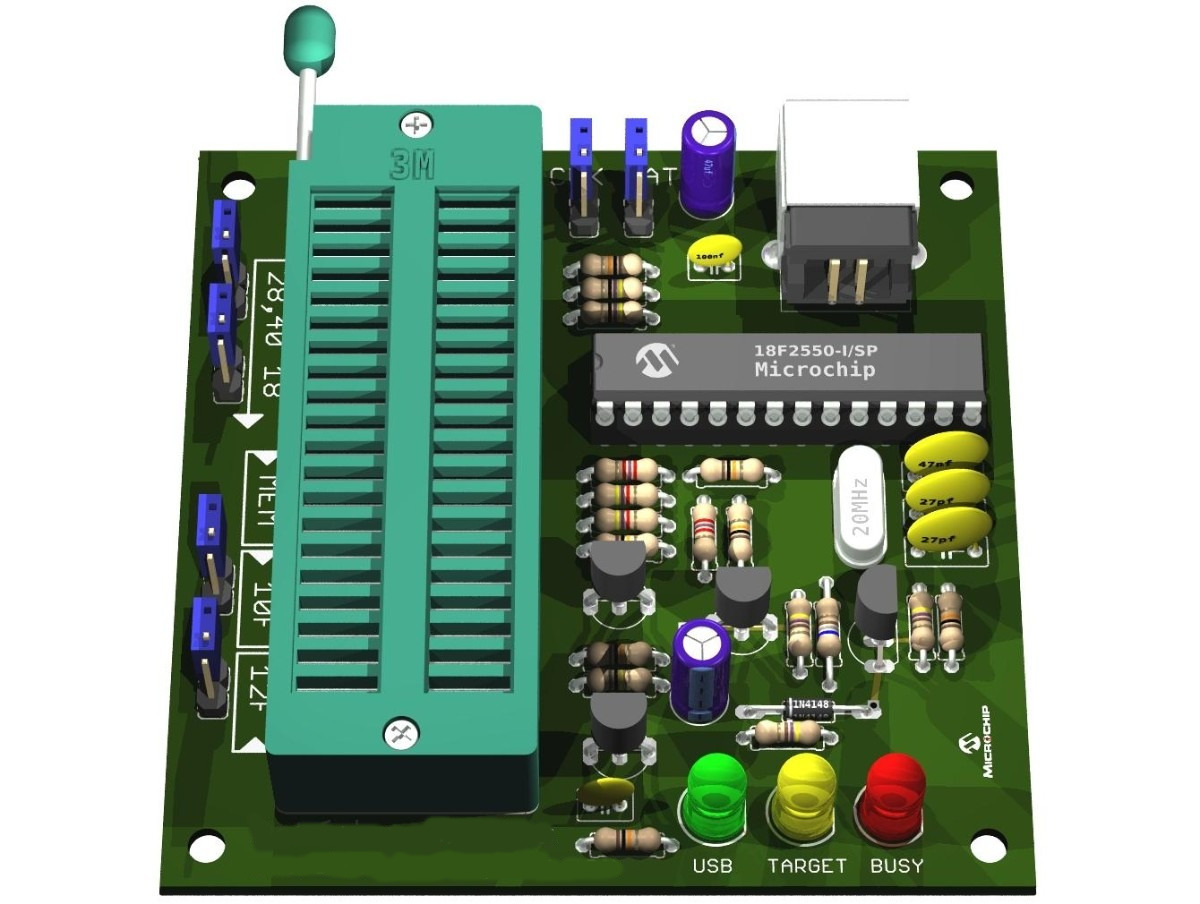
\includegraphics[scale=0.2]{images/company/modulo-programador-pic.jpg}
      \caption{Módulo Programador PIC}
      \label{fig:modulo-programador-pic}
    \end{figure}
    \begin{figure}[h!]
      \centering
      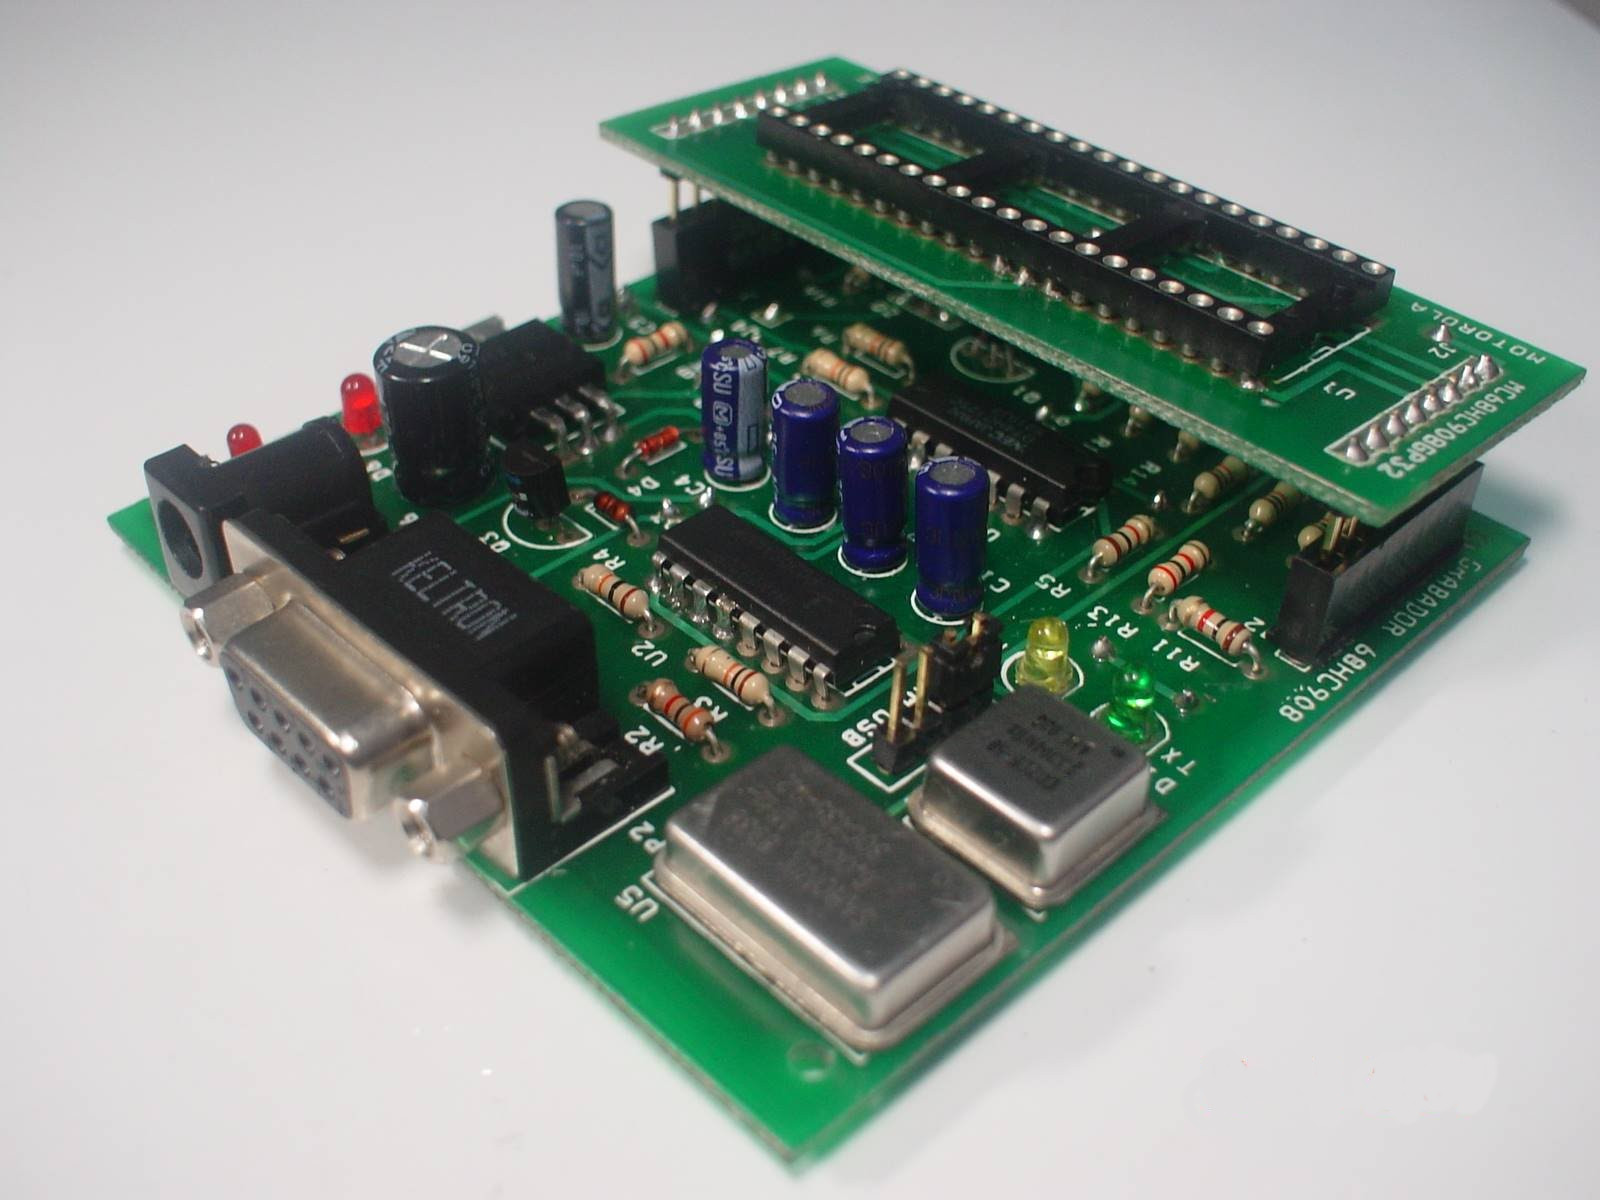
\includegraphics[scale=0.15]{images/company/modulo-programador-motorola.jpg}
      \caption{Módulo Programador Motorola}
      \label{fig:modulo-programador-motorola}
    \end{figure}
  \item Módulo entrenador para microcontroladores. Ver figura ~\ref{fig:entrenador-pic}.
    \begin{figure}[h!]
      \centering
      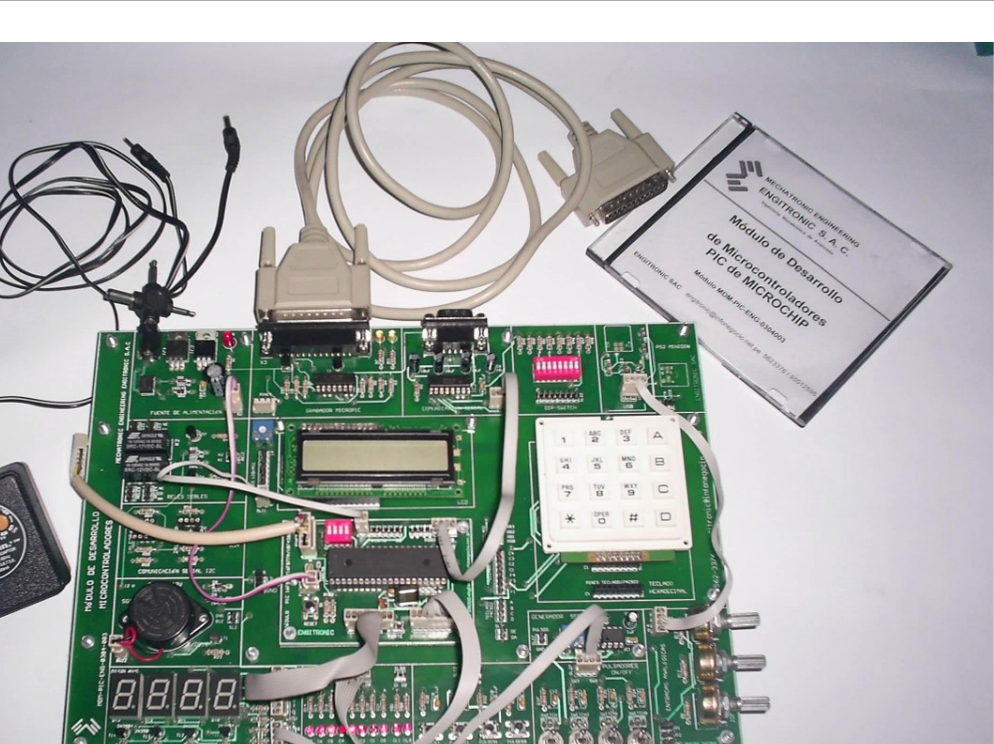
\includegraphics[scale=0.2]{images/company/entrenador-pic.png}
      \caption{Módulo entrenador para microcontroladores}
      \label{fig:entrenador-pic}
    \end{figure}
  \item Circuitos de telecomunicaciones. Ver figura ~\ref{fig:modulo-gps}. 
    \begin{figure}[h!]
      \centering
      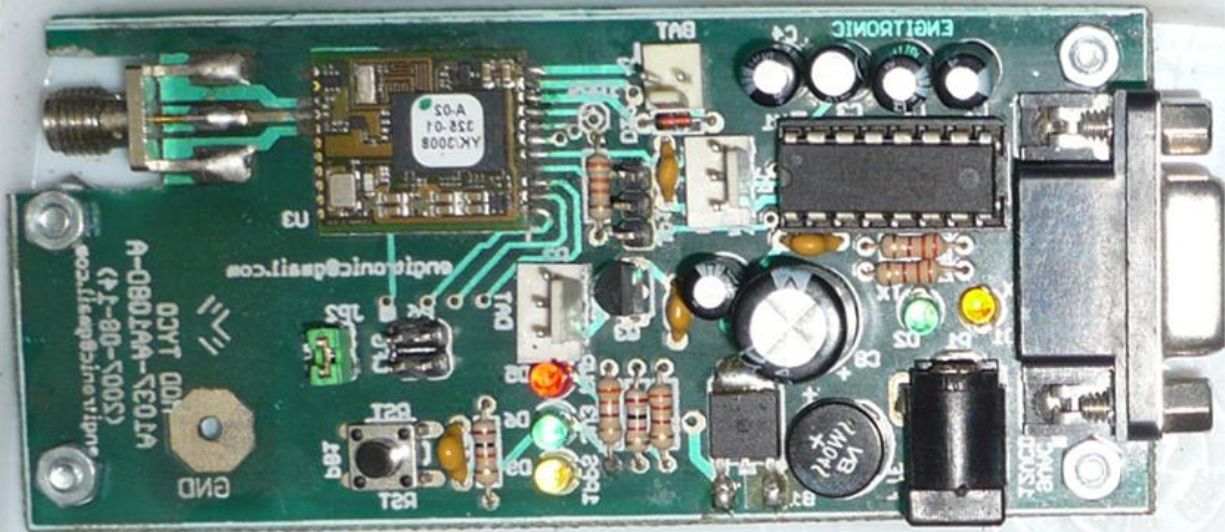
\includegraphics[scale=0.2]{images/company/modulo-gps.png}
      \caption{Módulo GPS 1080}
      \label{fig:modulo-gps}
    \end{figure}
\end{itemize}

\subsection{Implementación de sistemas para automatización}
Módulos de entrenamiento para PLCs. Ver figura ~\ref{fig:modulo-plc}. 
\begin{figure}[h!]
  \centering
  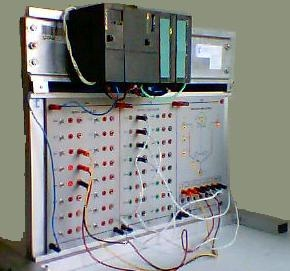
\includegraphics[scale=0.8]{images/company/modulo-plc.jpg}
  \caption{PLC Siemens}
  \label{fig:modulo-plc}
\end{figure}

\subsection{Diseño e implementación de sistemas robóticos}
\begin{itemize}
  \item Manipuladores Robóticos de propósito educativo.
  \item Robots seguidores de línea.
  \item Robots seguidores de luz.
  \item Robots móviles telecontrolados.
\end{itemize}

\subsection{Capacitaciones}
\begin{itemize}
  \item Curso de capacitación en programación de sistemas embebidos. Ver figura ~\ref{fig:capacitaciones}.
    \begin{figure}[h!]
      \centering
      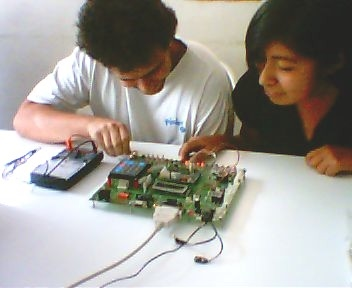
\includegraphics[scale=0.5]{images/company/capacitaciones.jpg}
      \caption{Capacitación en sistemas embebidos}
      \label{fig:capacitaciones}
    \end{figure}
  \item Visual C\# para aplicaciones con microcontroladores.
  \item C para microcontroladores PIC.
  \item C para microcontroladores MOTOROLA, Aplicaciones en Robótica y
  Radiofrecuencia.
  \item Introducción a la robótica.
  \item Automatización Industrial.
\end{itemize}

\subsection{Venta de equipos electrónicos y de telecomunicaciones}
\begin{itemize}
  \item Antenas GPRS.
  \item Módulos de desarrollo para microcontroladores.
  \item Circuitos electrónicos.
  \item Exportación de software especializado.
\end{itemize}


\section{Localización}
Dirección del Domicilio Fiscal: CAL. LUIS ROMERO NRO. 1025 URB. ROMA (ALT CDRA 26 AV COLONIAL) LIMA - LIMA - LIMA \\
Referencia: Cruce de la Av. Colonial y la Av. Universitaria.


\section{Infraestructura Productiva}

Las instalaciones de la empresa cuentan con un Almacén, un área de mecánica, un área de electrónica, un área de desarrollo de proyectos y una nueva área de cómputo implementada durante la práctica.

Los equipos disponibles en la empresa son:

\begin{itemize}
  \item Taladro de mesa. Ver figura ~\ref{fig:taladro-mesa}.
    \begin{figure}[h!]
      \centering
      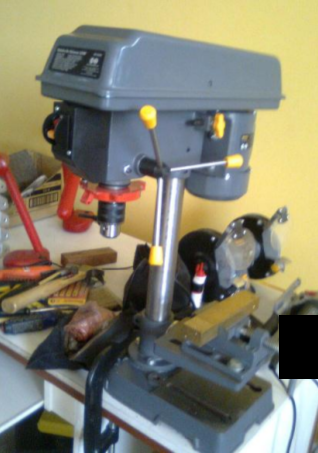
\includegraphics[scale=0.5]{images/company/taladro-mesa.png}
      \caption{Taladro de mesa}
      \label{fig:taladro-mesa}
    \end{figure}
  \item Esmeril. Ver figura ~\ref{fig:esmeril}.
    \begin{figure}[h!]
      \centering
      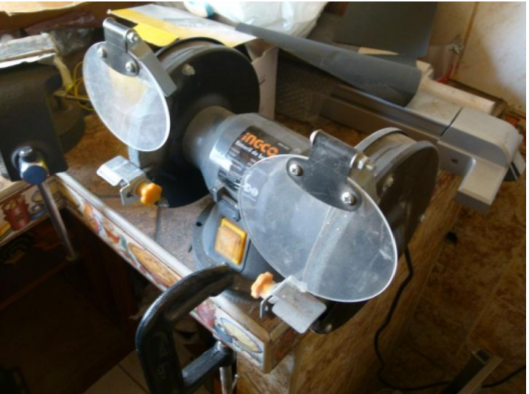
\includegraphics[scale=0.5]{images/company/esmeril.png}
      \caption{Esmeril}
      \label{fig:esmeril}
    \end{figure}
  \item Sierra Eléctrica. Ver figura ~\ref{fig:sierra-electrica}.
    \begin{figure}[h!]
      \centering
      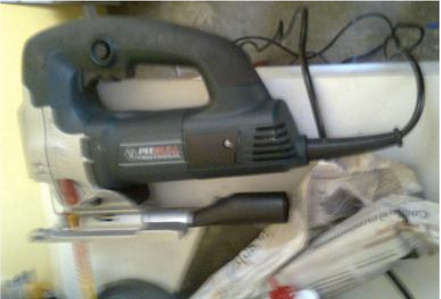
\includegraphics[scale=0.5]{images/company/sierra-electrica.png}
      \caption{Sierra Eléctrica}
      \label{fig:sierra-electrica}
    \end{figure}
  \item Prensa de banco. Ver figura ~\ref{fig:prensa-banco}.
    \begin{figure}[h!]
      \centering
      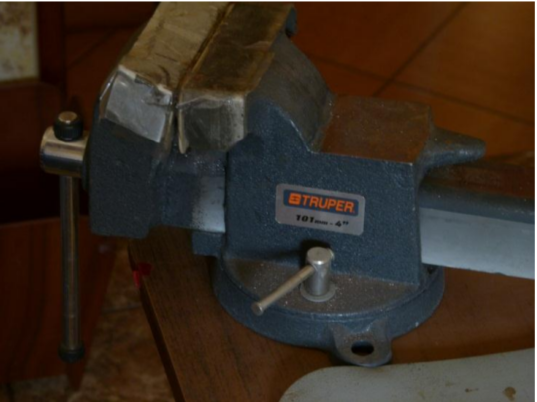
\includegraphics[scale=0.5]{images/company/prensa-banco.png}
      \caption{Prensa de banco}
      \label{fig:prensa-banco}
    \end{figure}
  \item Caja de circuitería electrónica. Ver figura ~\ref{fig:componentes-electronicos}.
    \begin{figure}[h!]
      \centering
      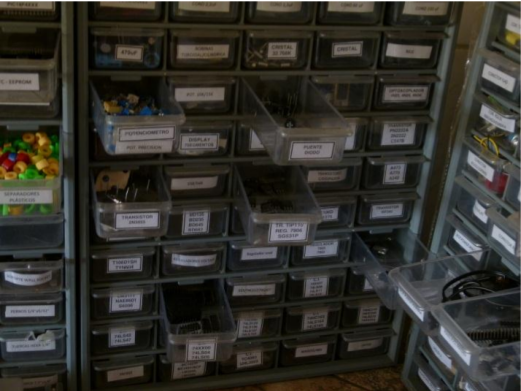
\includegraphics[scale=0.5]{images/company/componentes-electronicos.png}
      \caption{Componentes electrónicos y varios}
      \label{fig:componentes-electronicos}
    \end{figure}
\end{itemize} %literature survey included in this
\chapter{Actividades Desarrolladas}
En este capítulo se presentarán las actividades realizadas durante la práctica, explicando en que consiste cada una de ellas y mostrando el proceso de aprendizaje obtenido.


\section{Proyectos de Electrónica}

Uno de los fundamentales pilares de la empresa es el desarrollo de módulos electrónicos. En la presente sección se presentarán los principales módulos desarrollados en mi trayecto por la empresa.


\subsection{Diseño e Implementación de un Conversor frecuencia/voltaje para un Motor marca Pololu}

Al realizar el control de velocidad de un motor DC (Ver figuras ~\ref{fig:motor-pololu-1} y ~\ref{fig:motor-pololu-2}) necesitamos una variable de control, siendo la más fácil de obtener la frecuencia que su encoder nos retorna mediante pulsos de onda cuadrada (Ver figura ~\ref{fig:motor-pololu-3}).

\begin{figure}[h!]
  \centering
  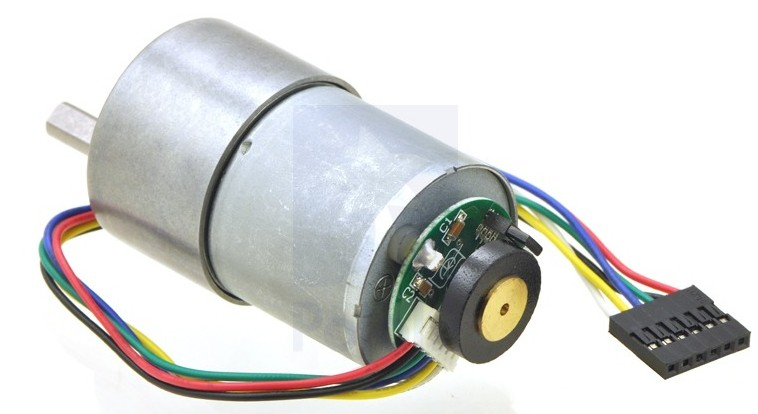
\includegraphics[scale=0.3]{images/activities/motor_pololu/motor1.jpg}
  \caption{Motor Pololu usado}
  \label{fig:motor-pololu-1}
\end{figure}

\begin{figure}[h!]
  \centering
  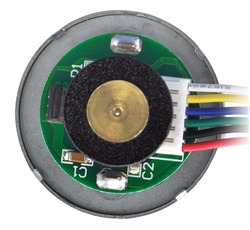
\includegraphics[scale=0.7]{images/activities/motor_pololu/motor2.jpg}
  \caption{Vista del encoder. Motor Pololu.}
  \label{fig:motor-pololu-2}
\end{figure}

\begin{figure}[h!]
  \centering
  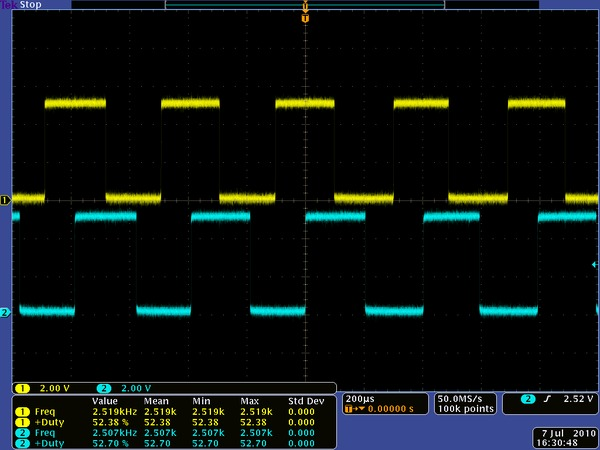
\includegraphics[scale=0.7]{images/activities/motor_pololu/motor3.jpg}
  \caption{Lectura de Encoders}
  \label{fig:motor-pololu-3}
\end{figure}

La frecuencia es convertida a voltaje análogo (mediante el circuito integrado LM331). el cual es fácil de procesar por un ADC (Conversor Análogo Digital) para finalmente poder tratar a la señal digital de forma discreta. Un esquema general se puede apreciar en la figura ~\ref{fig:esquema-control-motor}.

\begin{figure}[h!]
  \centering
  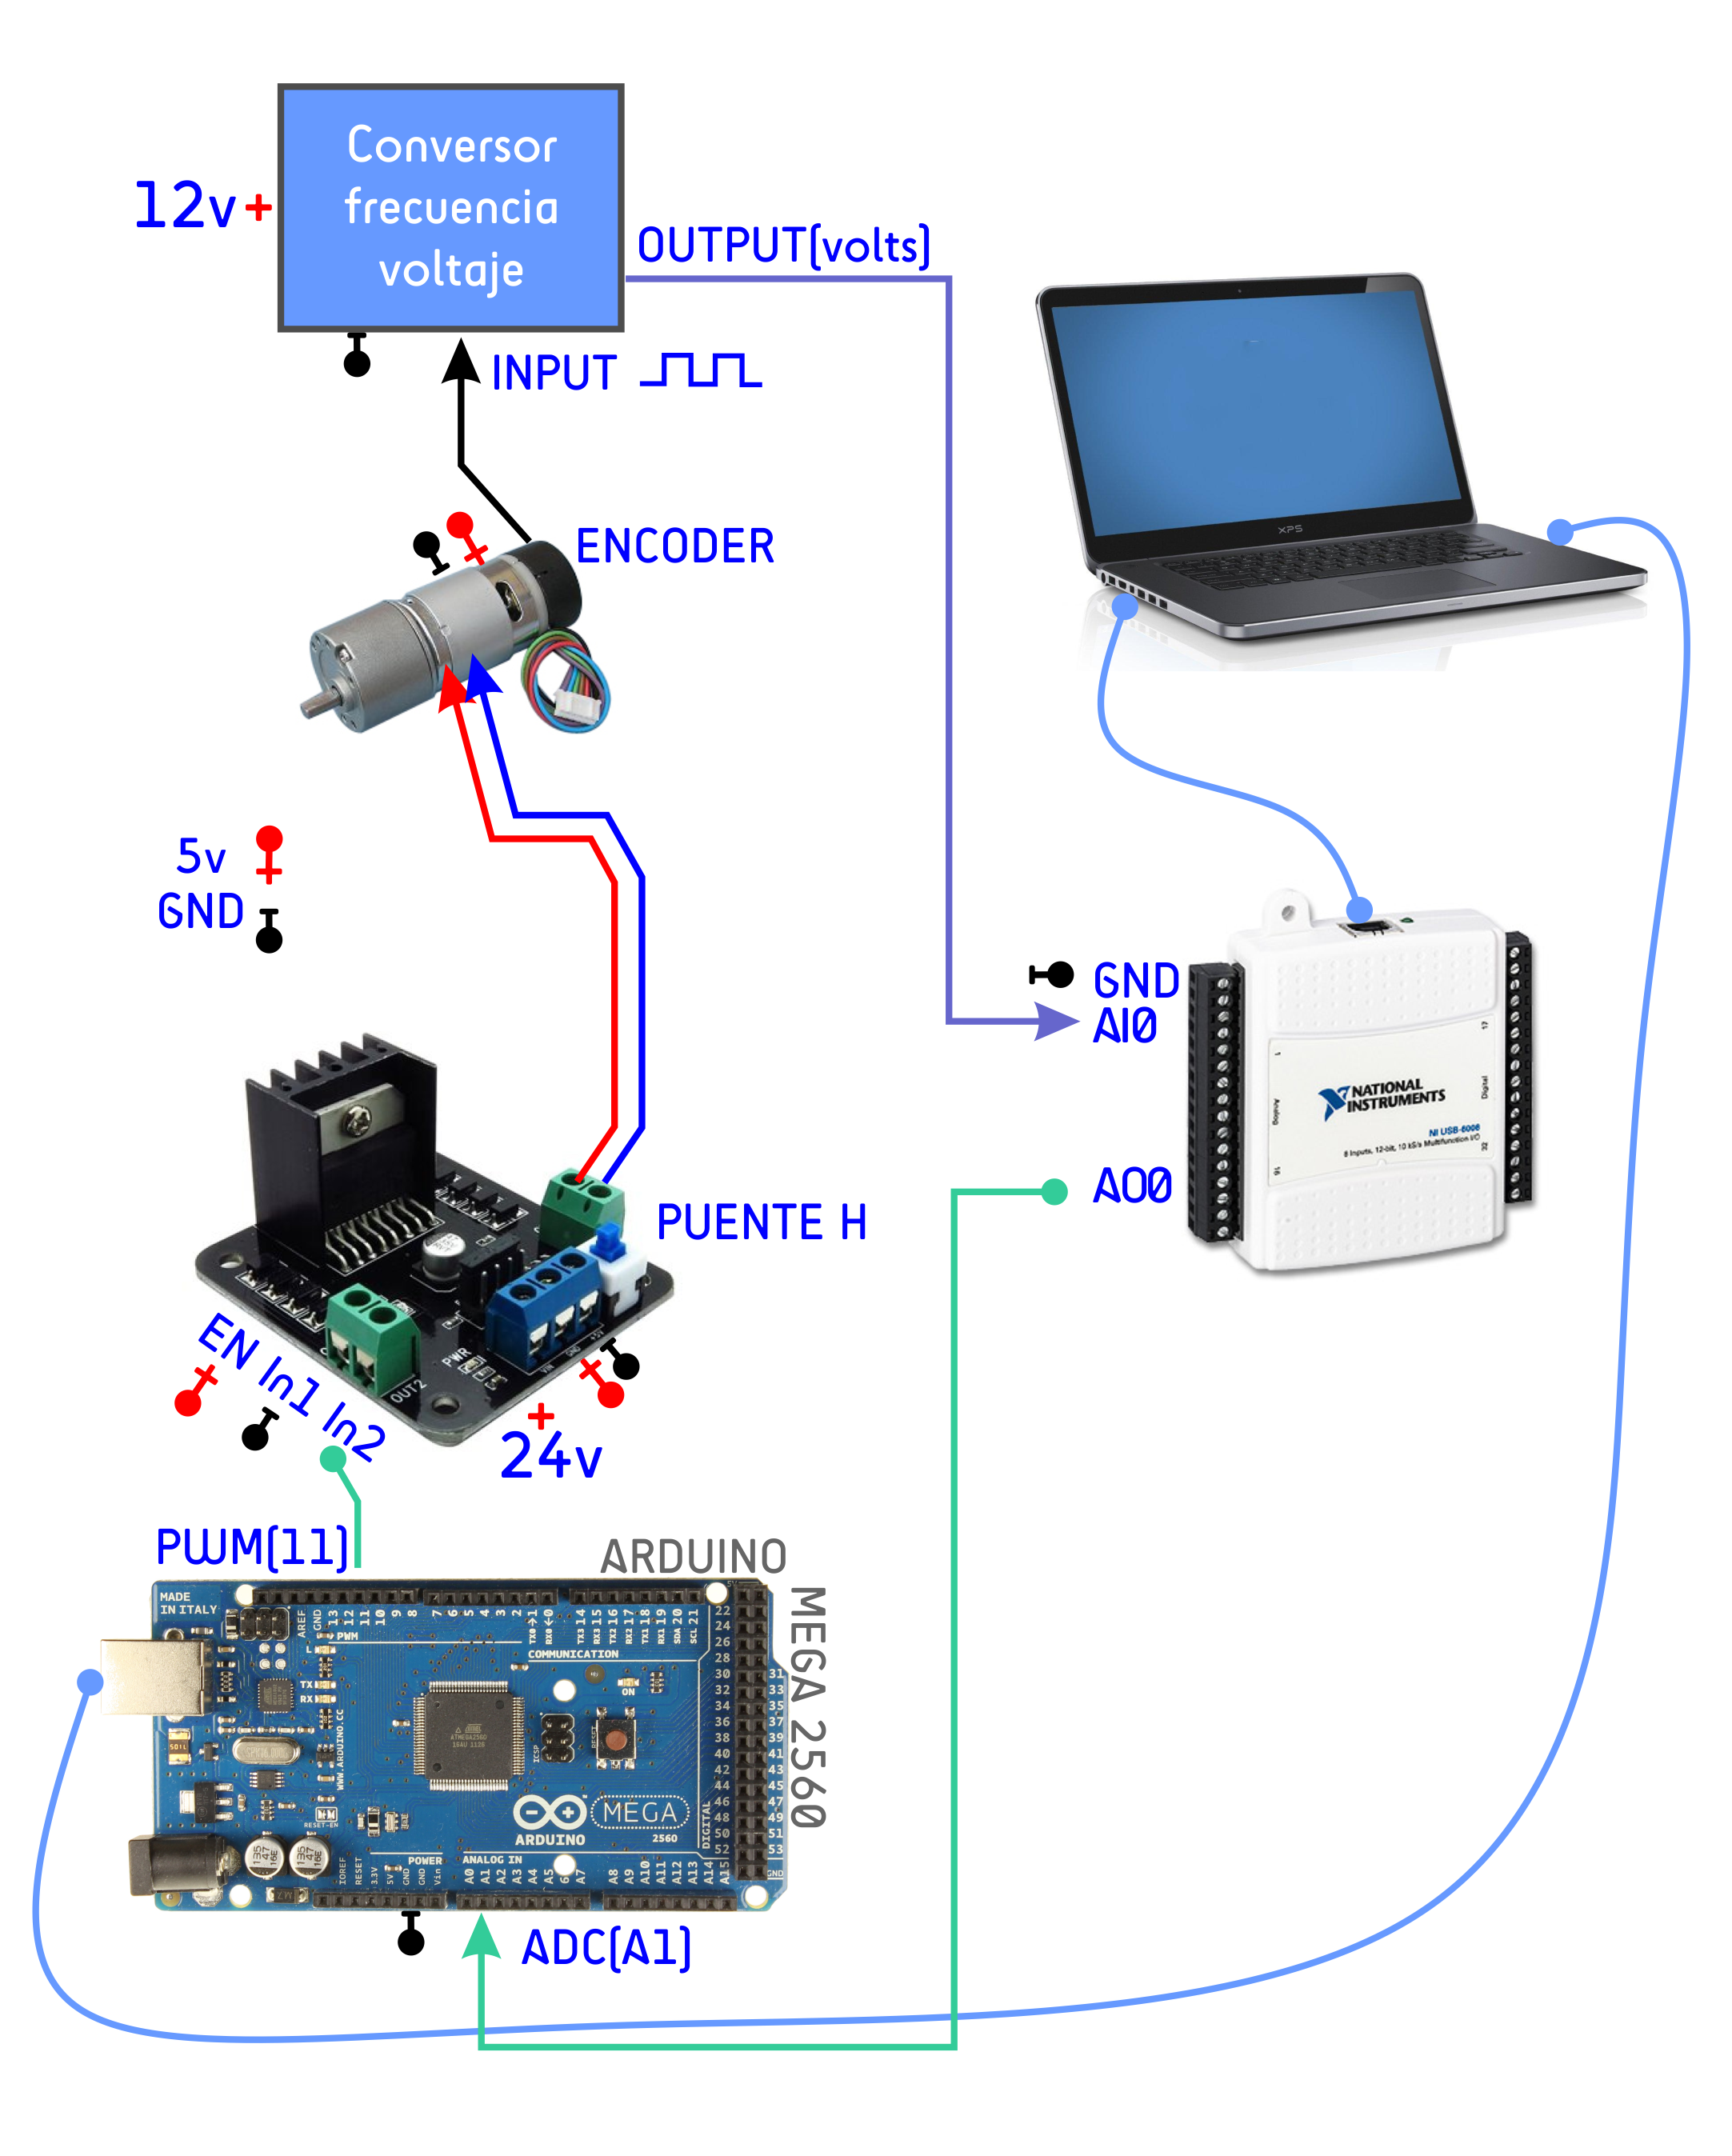
\includegraphics[scale=0.7]{images/activities/motor_pololu/esquema-control-motor.png}
  \caption{Diagrama de control de velocidad de un motor DC}
  \label{fig:esquema-control-motor}
\end{figure}

El circuito fue diseñado para poder ser usado por una DAQ de la empresa National Instruments (Ver figura ~\ref{fig:daq}) o un launchpad TIVA (Ver figura ~\ref{fig:tiva}) como controlador. Por ello se consideró que el voltaje de salida del conversor f/v sea escalado hasta 3.5v (voltaje de saturación mínimo del ADC de ambos controladores).

\begin{figure}[h!]
  \centering
  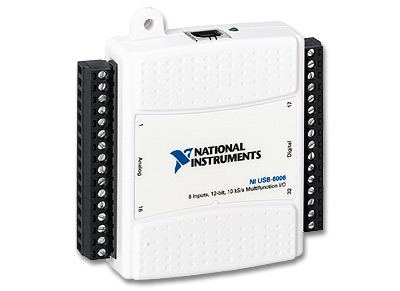
\includegraphics[scale=0.6]{images/activities/daq/daq.jpg}
  \caption{DAQ de National Instruments USB-6008, es un un dispositivo de adquisición de datos de bajo costo.}
  \label{fig:daq}
\end{figure}

\begin{figure}[h!]
  \centering
  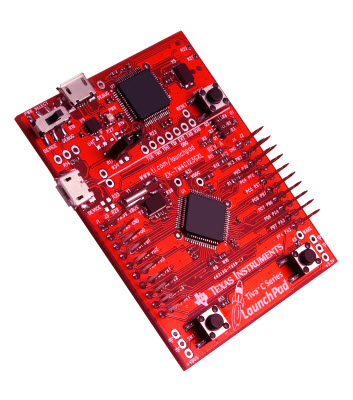
\includegraphics[scale=1.5]{images/activities/motor_pololu/tiva.jpg}
  \caption{Tiva™ C Series LaunchPad Evaluation Kit. El LaunchPad Tiva es una plataforma de evaluación de bajo costo para microcontroladores ARM Cortex M4F de Texas Instruments}
  \label{fig:tiva}
\end{figure}

De las condiciones establecidas, obtuvimos el siguiente diseño realizando los cálculos establecidos en el datasheet del C.I. LM331. Ver figura ~\ref{fig:schematic-motor-pololu}.

\begin{figure}[h!]
  \centering
  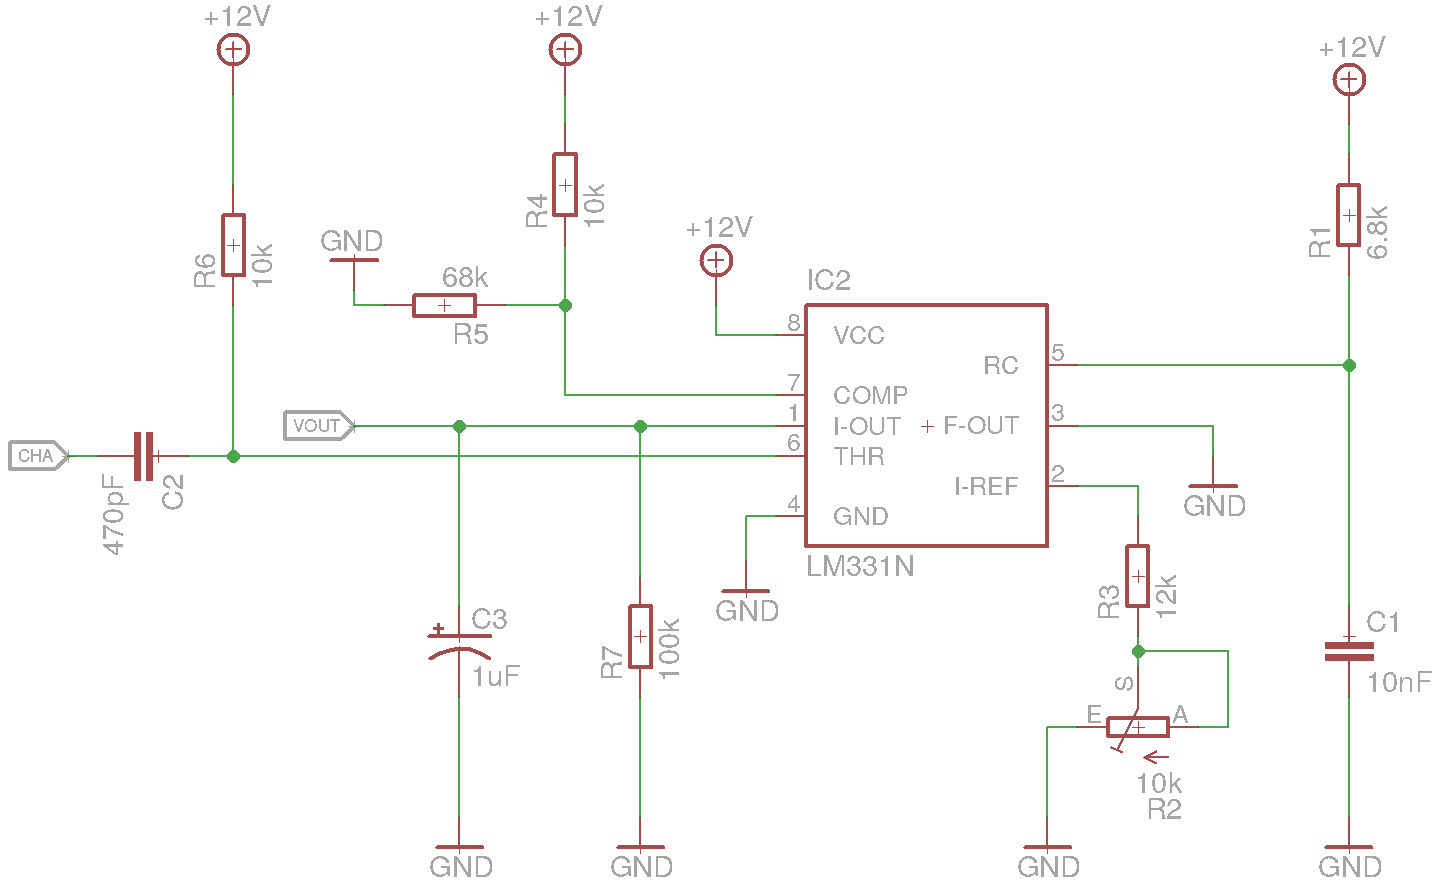
\includegraphics[scale=0.3]{images/activities/motor_pololu/schematic-motor-pololu.png}
  \caption{Esquemático del circuito diseñado}
  \label{fig:schematic-motor-pololu}
\end{figure}

Asi mismo el pcb (board) del circuito final es el que se aprecia en la figura ~\ref{fig:board-motor-pololu} en la cual se observa las entradas y salidas del módulo, así como también la incorporación de un socket especial para un Arduino nano.

\begin{figure}[h!]
  \centering
  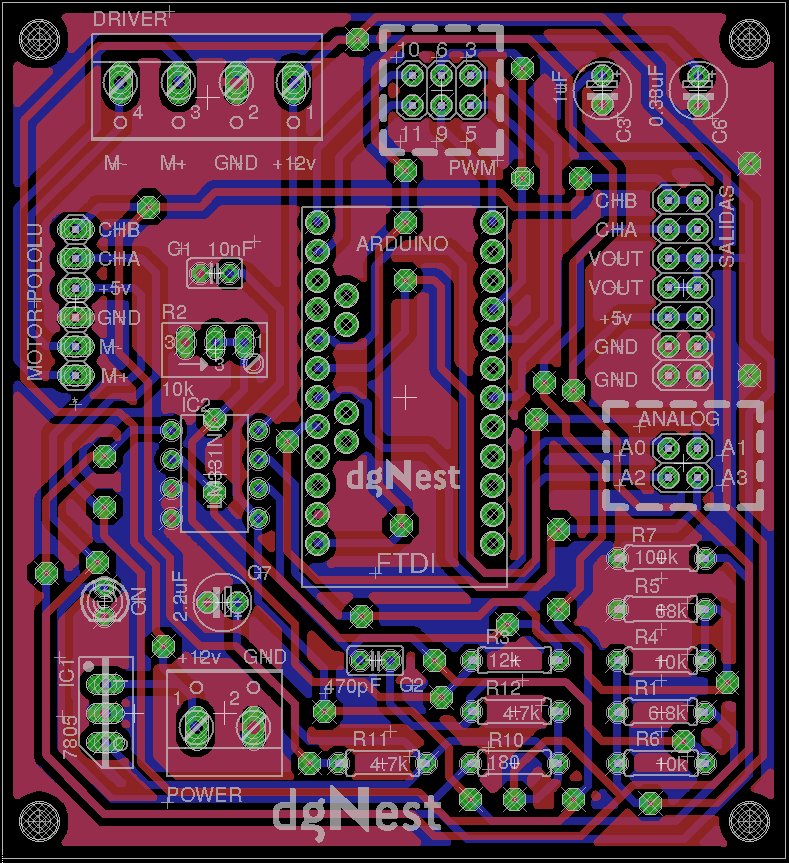
\includegraphics[scale=0.3]{images/activities/motor_pololu/board-motor-pololu.png}
  \caption{PCB (board) conversor f/v generado en eagle}
  \label{fig:board-motor-pololu}
\end{figure}

Por política de la empresa, siempre se realizan prueban de los módulo antes de salir al mercado. En las figura ~\ref{fig:pruebas-motor-pololu} se pueda observar dicho proceso.

\begin{figure}
  \centering
  \begin{subfigure}{0.45\textwidth}
    \centering
    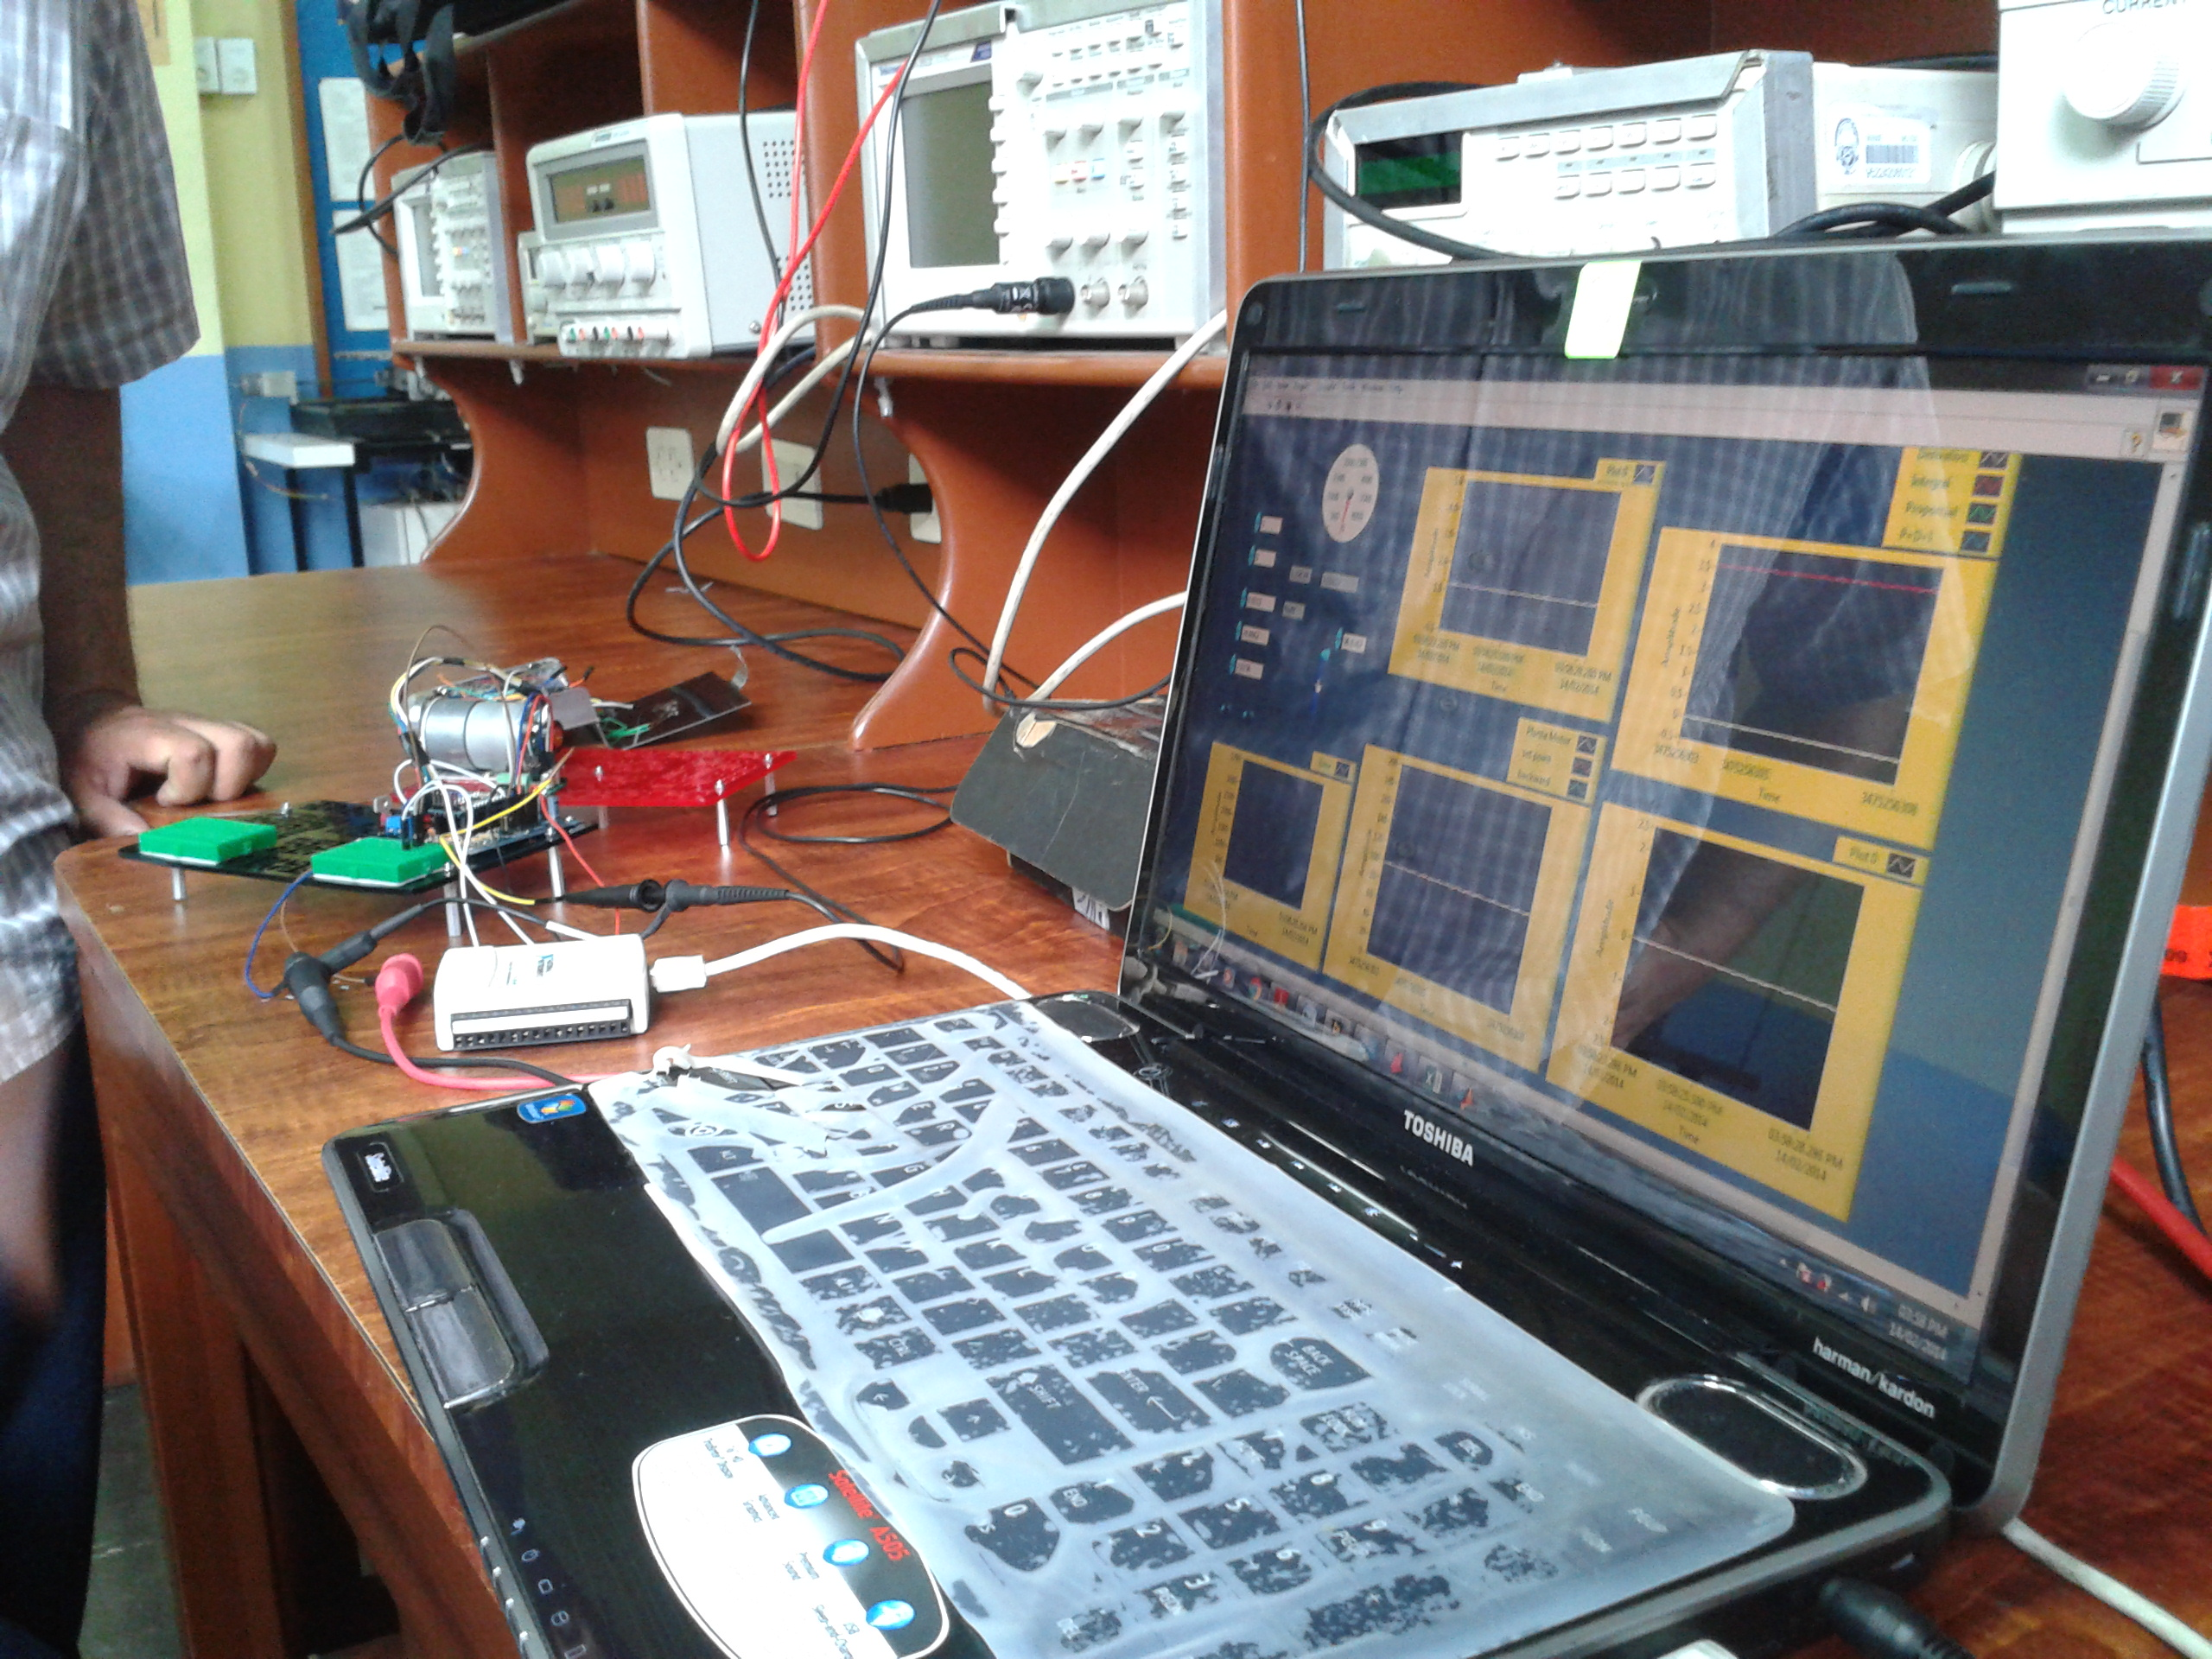
\includegraphics[scale=0.065]{images/activities/motor_pololu/pruebas-control-velocidad.jpg}
  \end{subfigure}
  % \hfill
  \begin{subfigure}{0.45\textwidth}
    \centering
    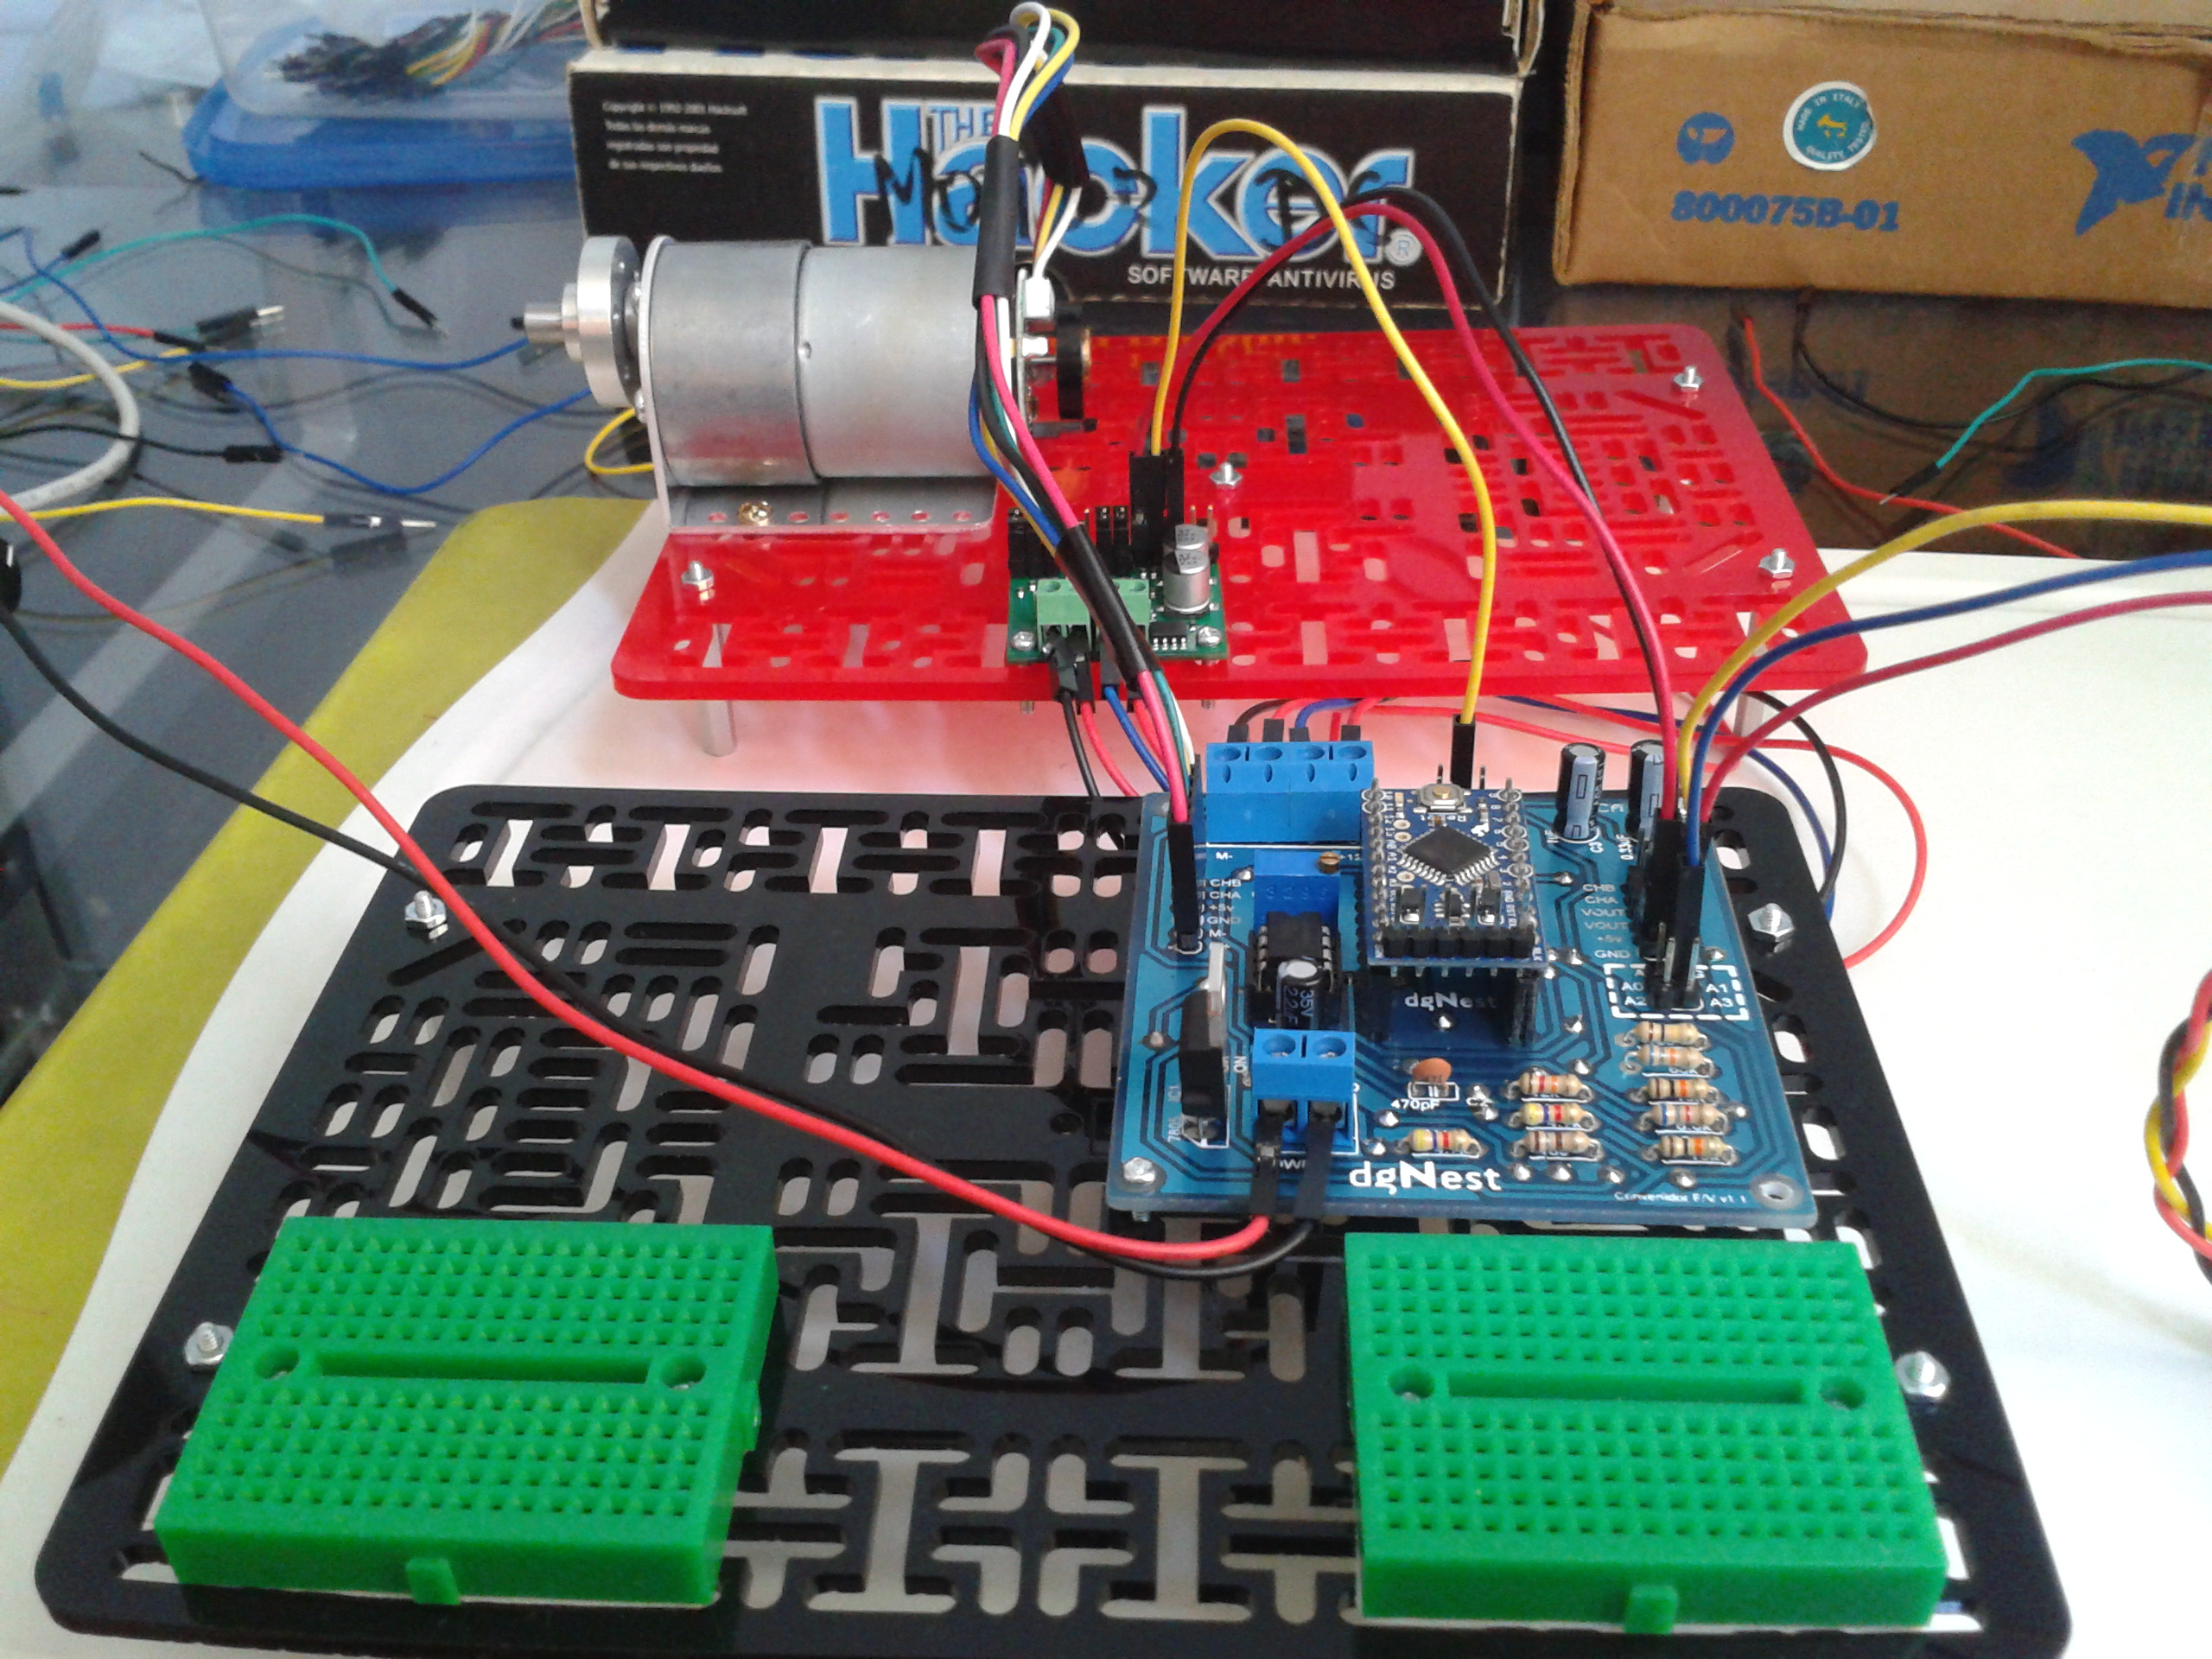
\includegraphics[scale=0.065]{images/activities/motor_pololu/pruebas-motor-pololu.jpg}
  \end{subfigure}
  \caption{Pruebas del módulo}
  \label{fig:pruebas-motor-pololu}
\end{figure}

El módulo resultante se puede observar en la figura ~\ref{fig:modulo-pololu}. El cual posteriormente se empaqueto y realizó la entrega respectiva (Ver figura ~\ref{fig:empaquetado-pololu}).

\begin{figure}[h!]
  \centering
  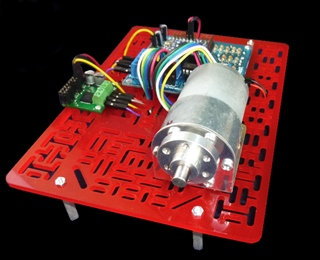
\includegraphics[scale=0.8]{images/activities/motor_pololu/modulo-pololu.png}
  \caption{Módulo conversor frecuencia voltaje terminado}
  \label{fig:modulo-pololu}
\end{figure}

\begin{figure}[h!]
  \centering
  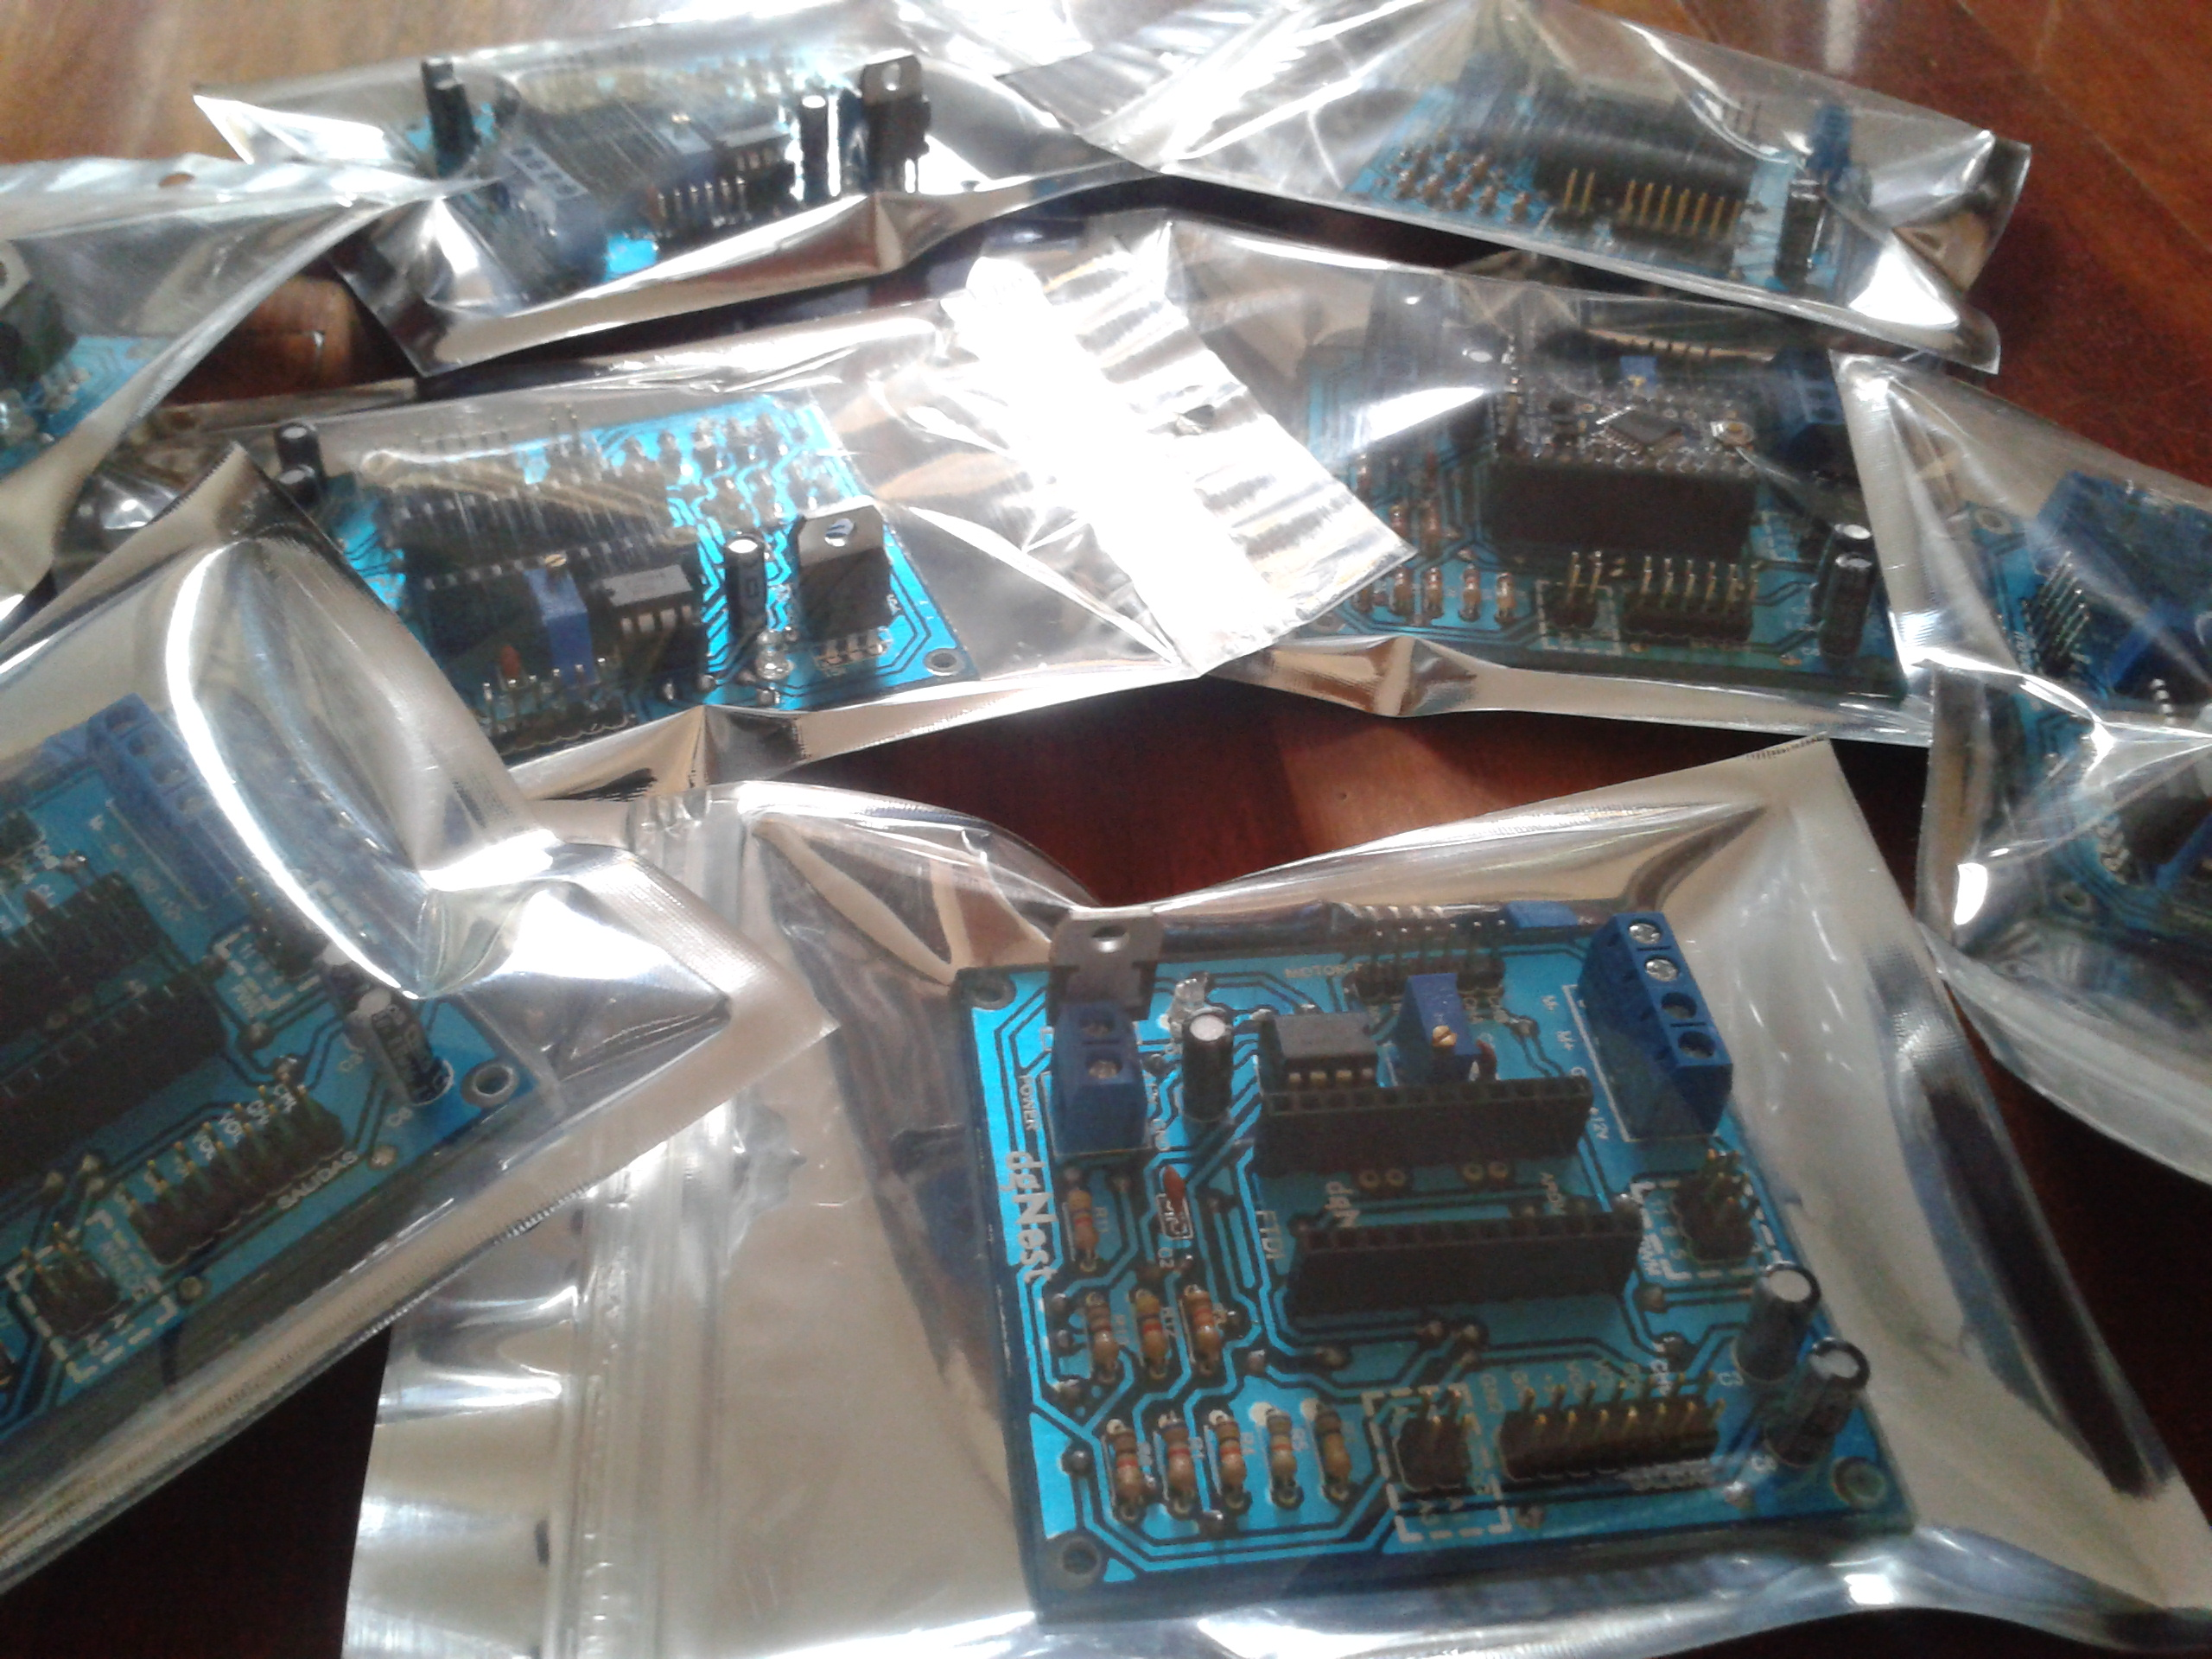
\includegraphics[scale=0.1]{images/activities/motor_pololu/empaquetado-pololu.jpg}
  \caption{Módulos empaquetados y listos para su distribución}
  \label{fig:empaquetado-pololu}
\end{figure}

\clearpage

\subsection{Diseño e Implementación de un modulo Conversor frecuencia/voltaje para un Motor EMG30 + Sensor de Corriente}

Este proyecto estuvo basado en la sección anterior. Con la salvedad que se rediseñaron los parámetros del circuito LM331 para el motor EMG30 (Ver figuras ~\ref{fig:schematic-board-motor-emg30}, ~\ref{fig:motor-emg30} y ~\ref{fig:board-motor-emg30}). Además sea agregó un sensor de corriente (ACS712) para hacer un modelamiento paramétrico del motor.

\begin{figure}[h!]
  \centering
  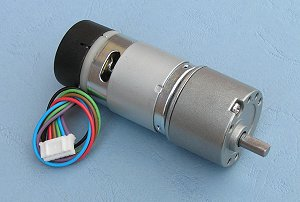
\includegraphics[scale=0.8]{images/activities/motor_emg30/motor-emg30.jpg}
  \caption{Motor EMG30}
  \label{fig:motor-emg30}
\end{figure}

\begin{figure}[h!]
  \centering
  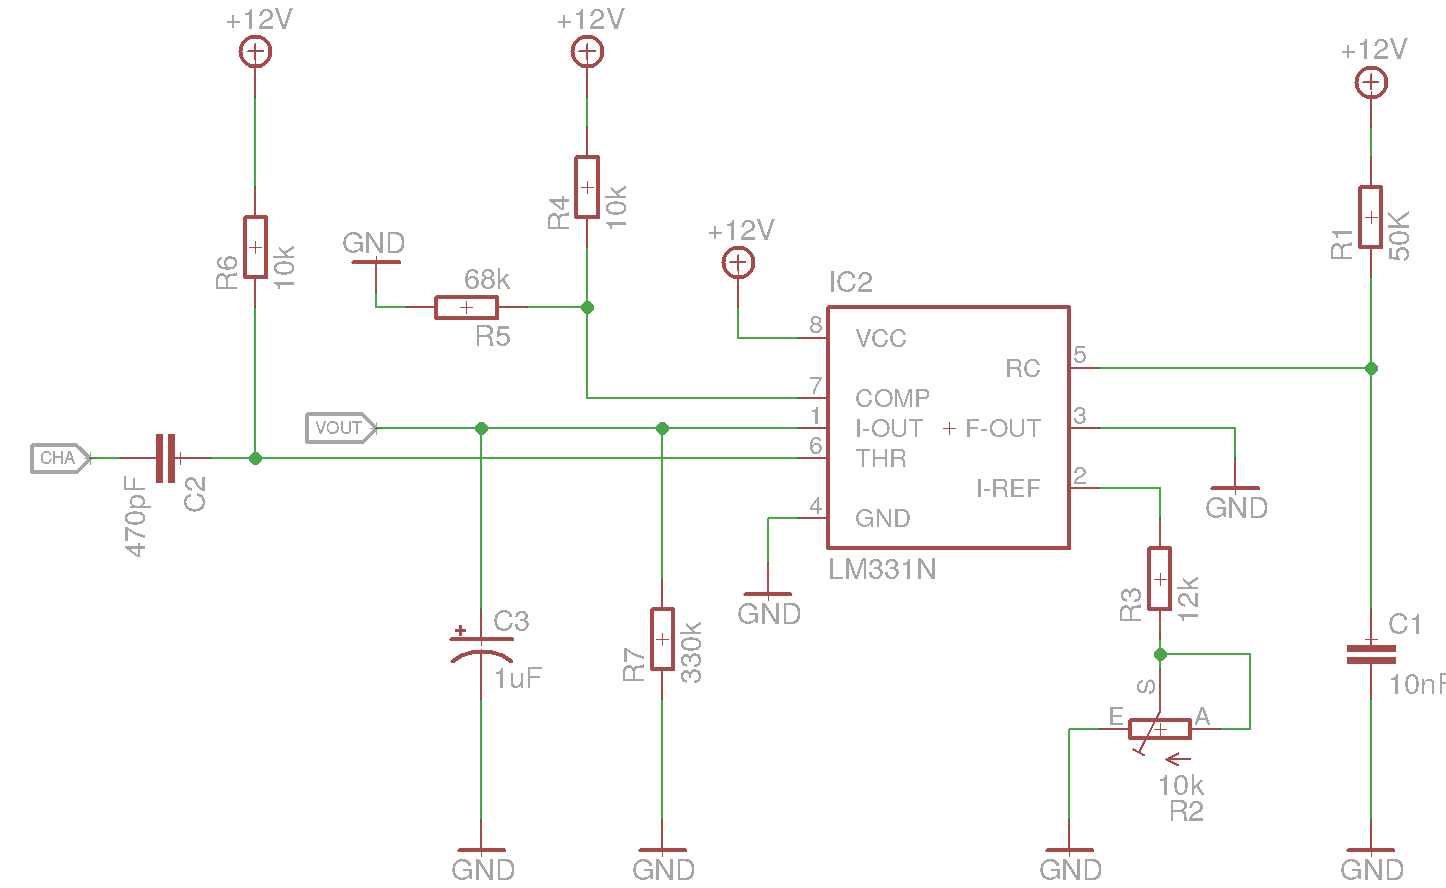
\includegraphics[scale=0.2]{images/activities/motor_emg30/schematic-board-motor-emg30.png}
  \caption{Esquemático del circuito LM331 diseñado para un motor EMG30}
  \label{fig:schematic-board-motor-emg30}
\end{figure}

\begin{figure}[h!]
  \centering
  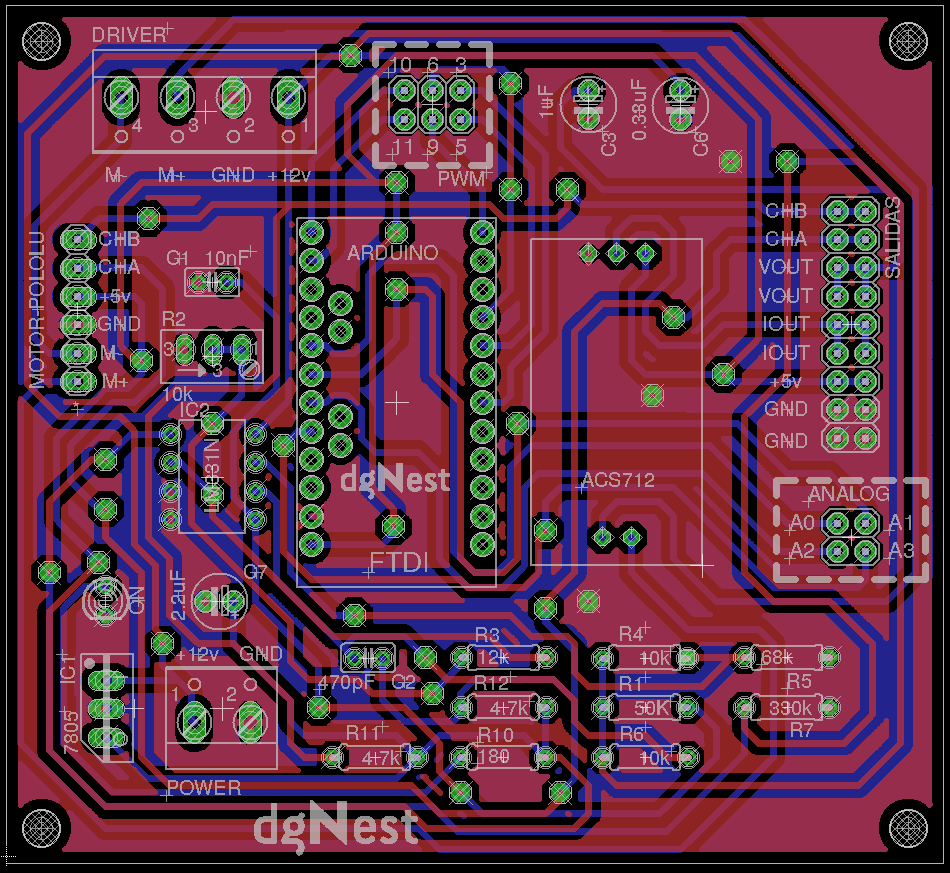
\includegraphics[scale=0.3]{images/activities/motor_emg30/board-motor-emg30.png}
  \caption{PCB (board) del circuito LM331 diseñado para un motor EMG30}
  \label{fig:board-motor-emg30}
\end{figure}

El módulo terminado puede ser apreciado en la figura ~\ref{fig:modulo-emg30-1}.

\begin{figure}[h!]
  \centering
  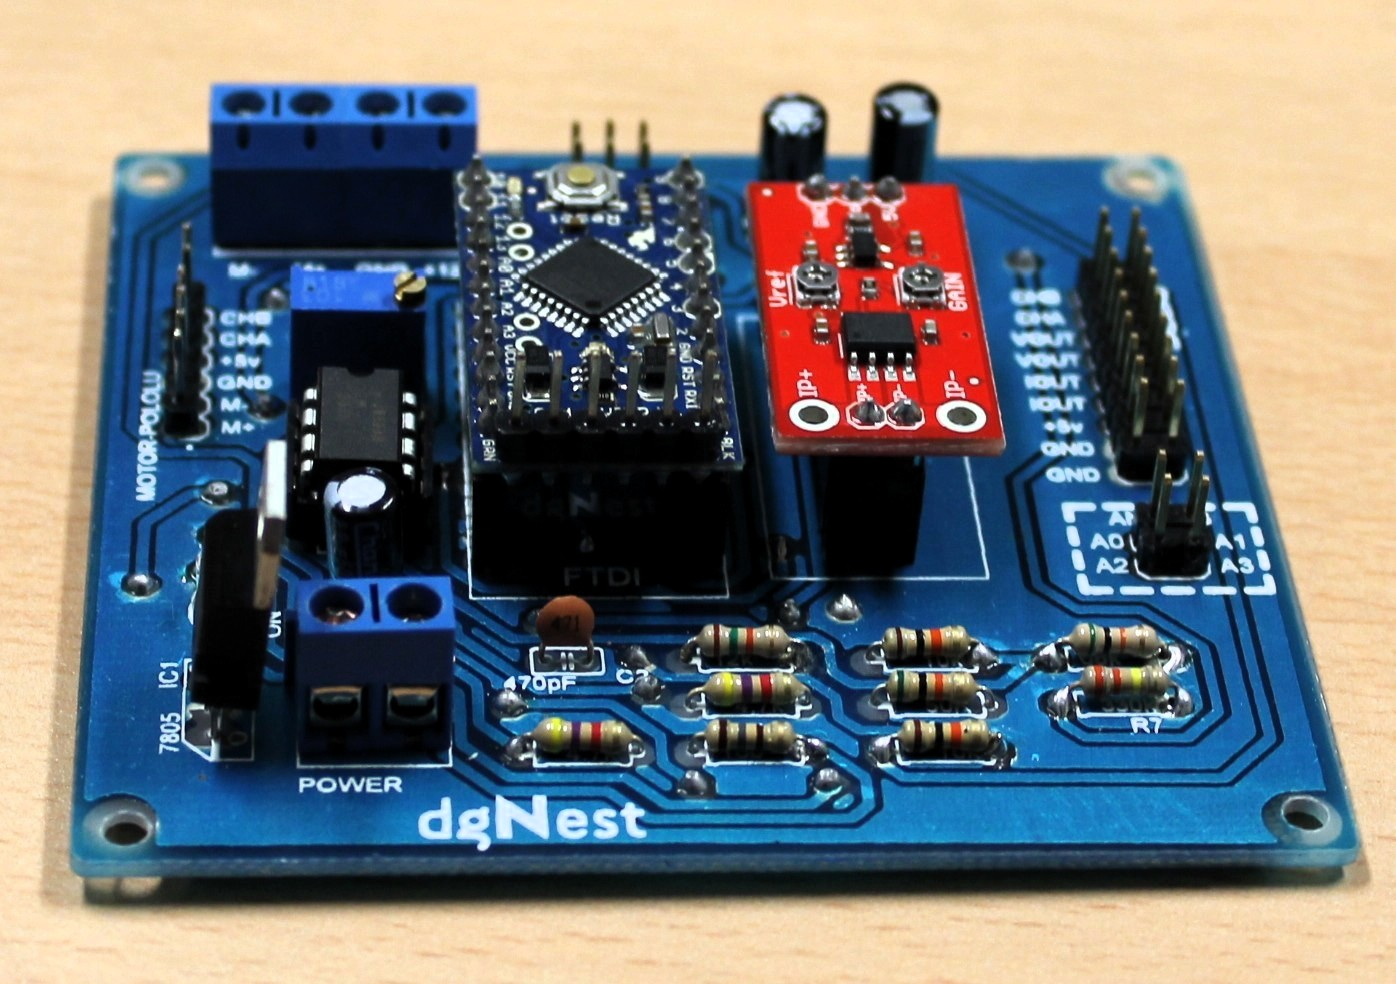
\includegraphics[scale=0.25]{images/activities/motor_emg30/modulo-emg30-1.jpg}
  \caption{Módulo conversor frecuencia voltaje terminado}
  \label{fig:modulo-emg30-1}
\end{figure}

\clearpage

\subsection{Diseño e Implementación de Plantas Analógicas}

Se diseño mediante el opam TL082 un circuito en dos modos, con el cual obtuvimos dos plantas. Una de primer orden y otra de segundo orden subamortiguado. Ver figuras ~\ref{fig:schematic-planta-TL082}, ~\ref{fig:board-planta-TL082} y ~\ref{fig:TL082}.

\begin{figure}[h!]
  \centering
  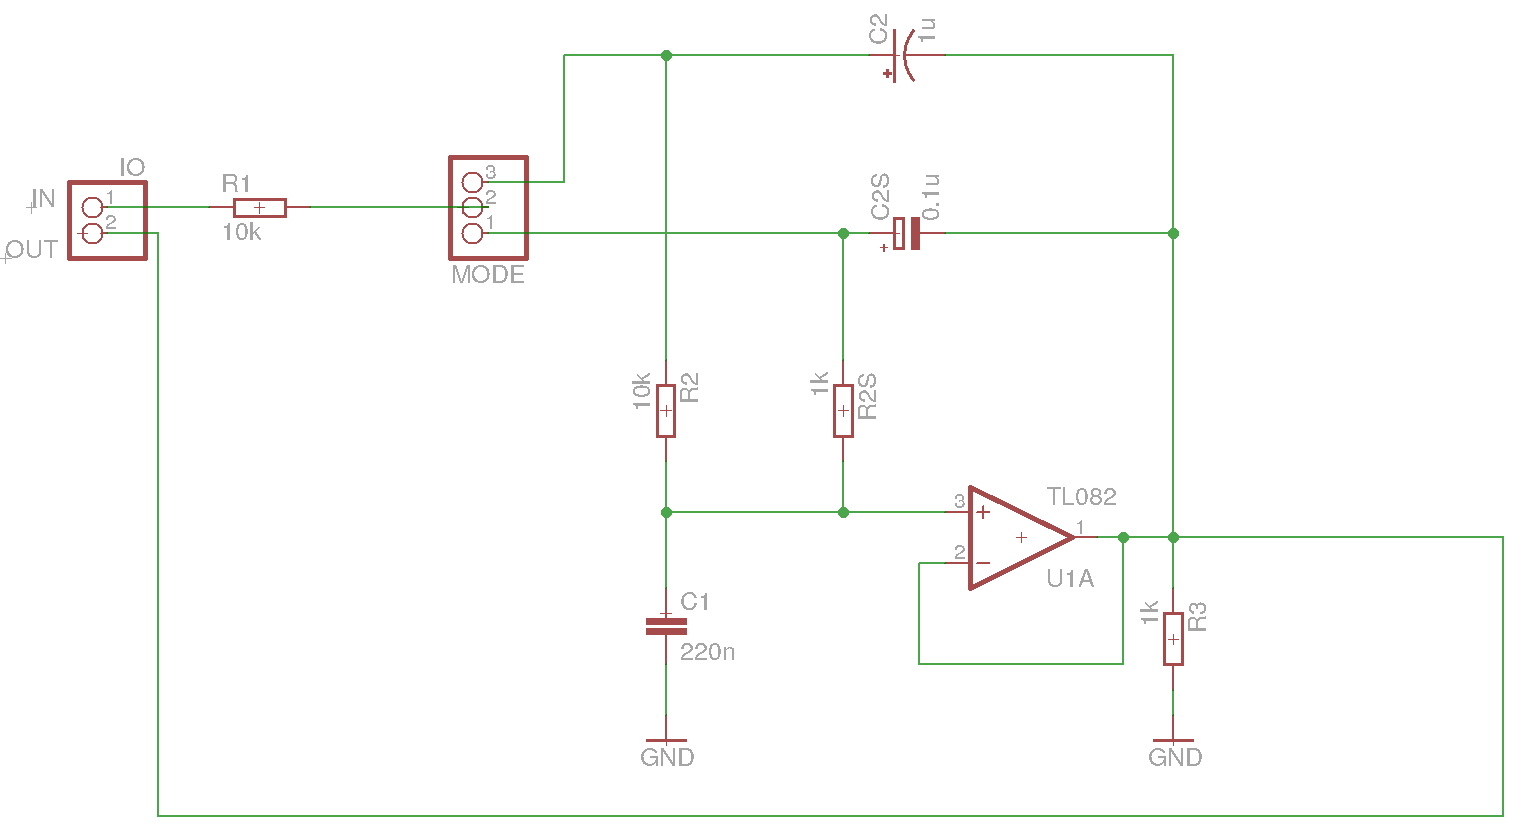
\includegraphics[scale=0.25]{images/activities/plantas_analogicas/schematic-planta-TL082.png}
  \caption{Esquemático de la planta TL082}
  \label{fig:schematic-planta-TL082}
\end{figure}

\begin{figure}[h!]
  \centering
  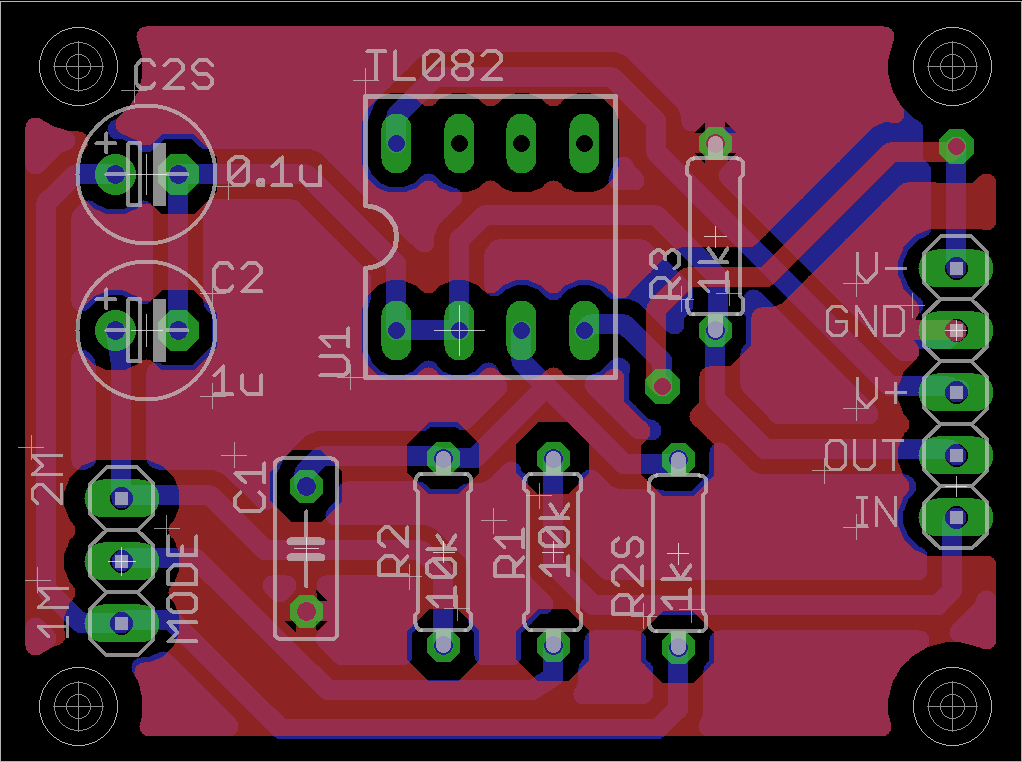
\includegraphics[scale=0.25]{images/activities/plantas_analogicas/board-planta-TL082.png}
  \caption{PCB (board) de la planta TL082}
  \label{fig:board-planta-TL082}
\end{figure}

\begin{figure}[h!]
  \centering
  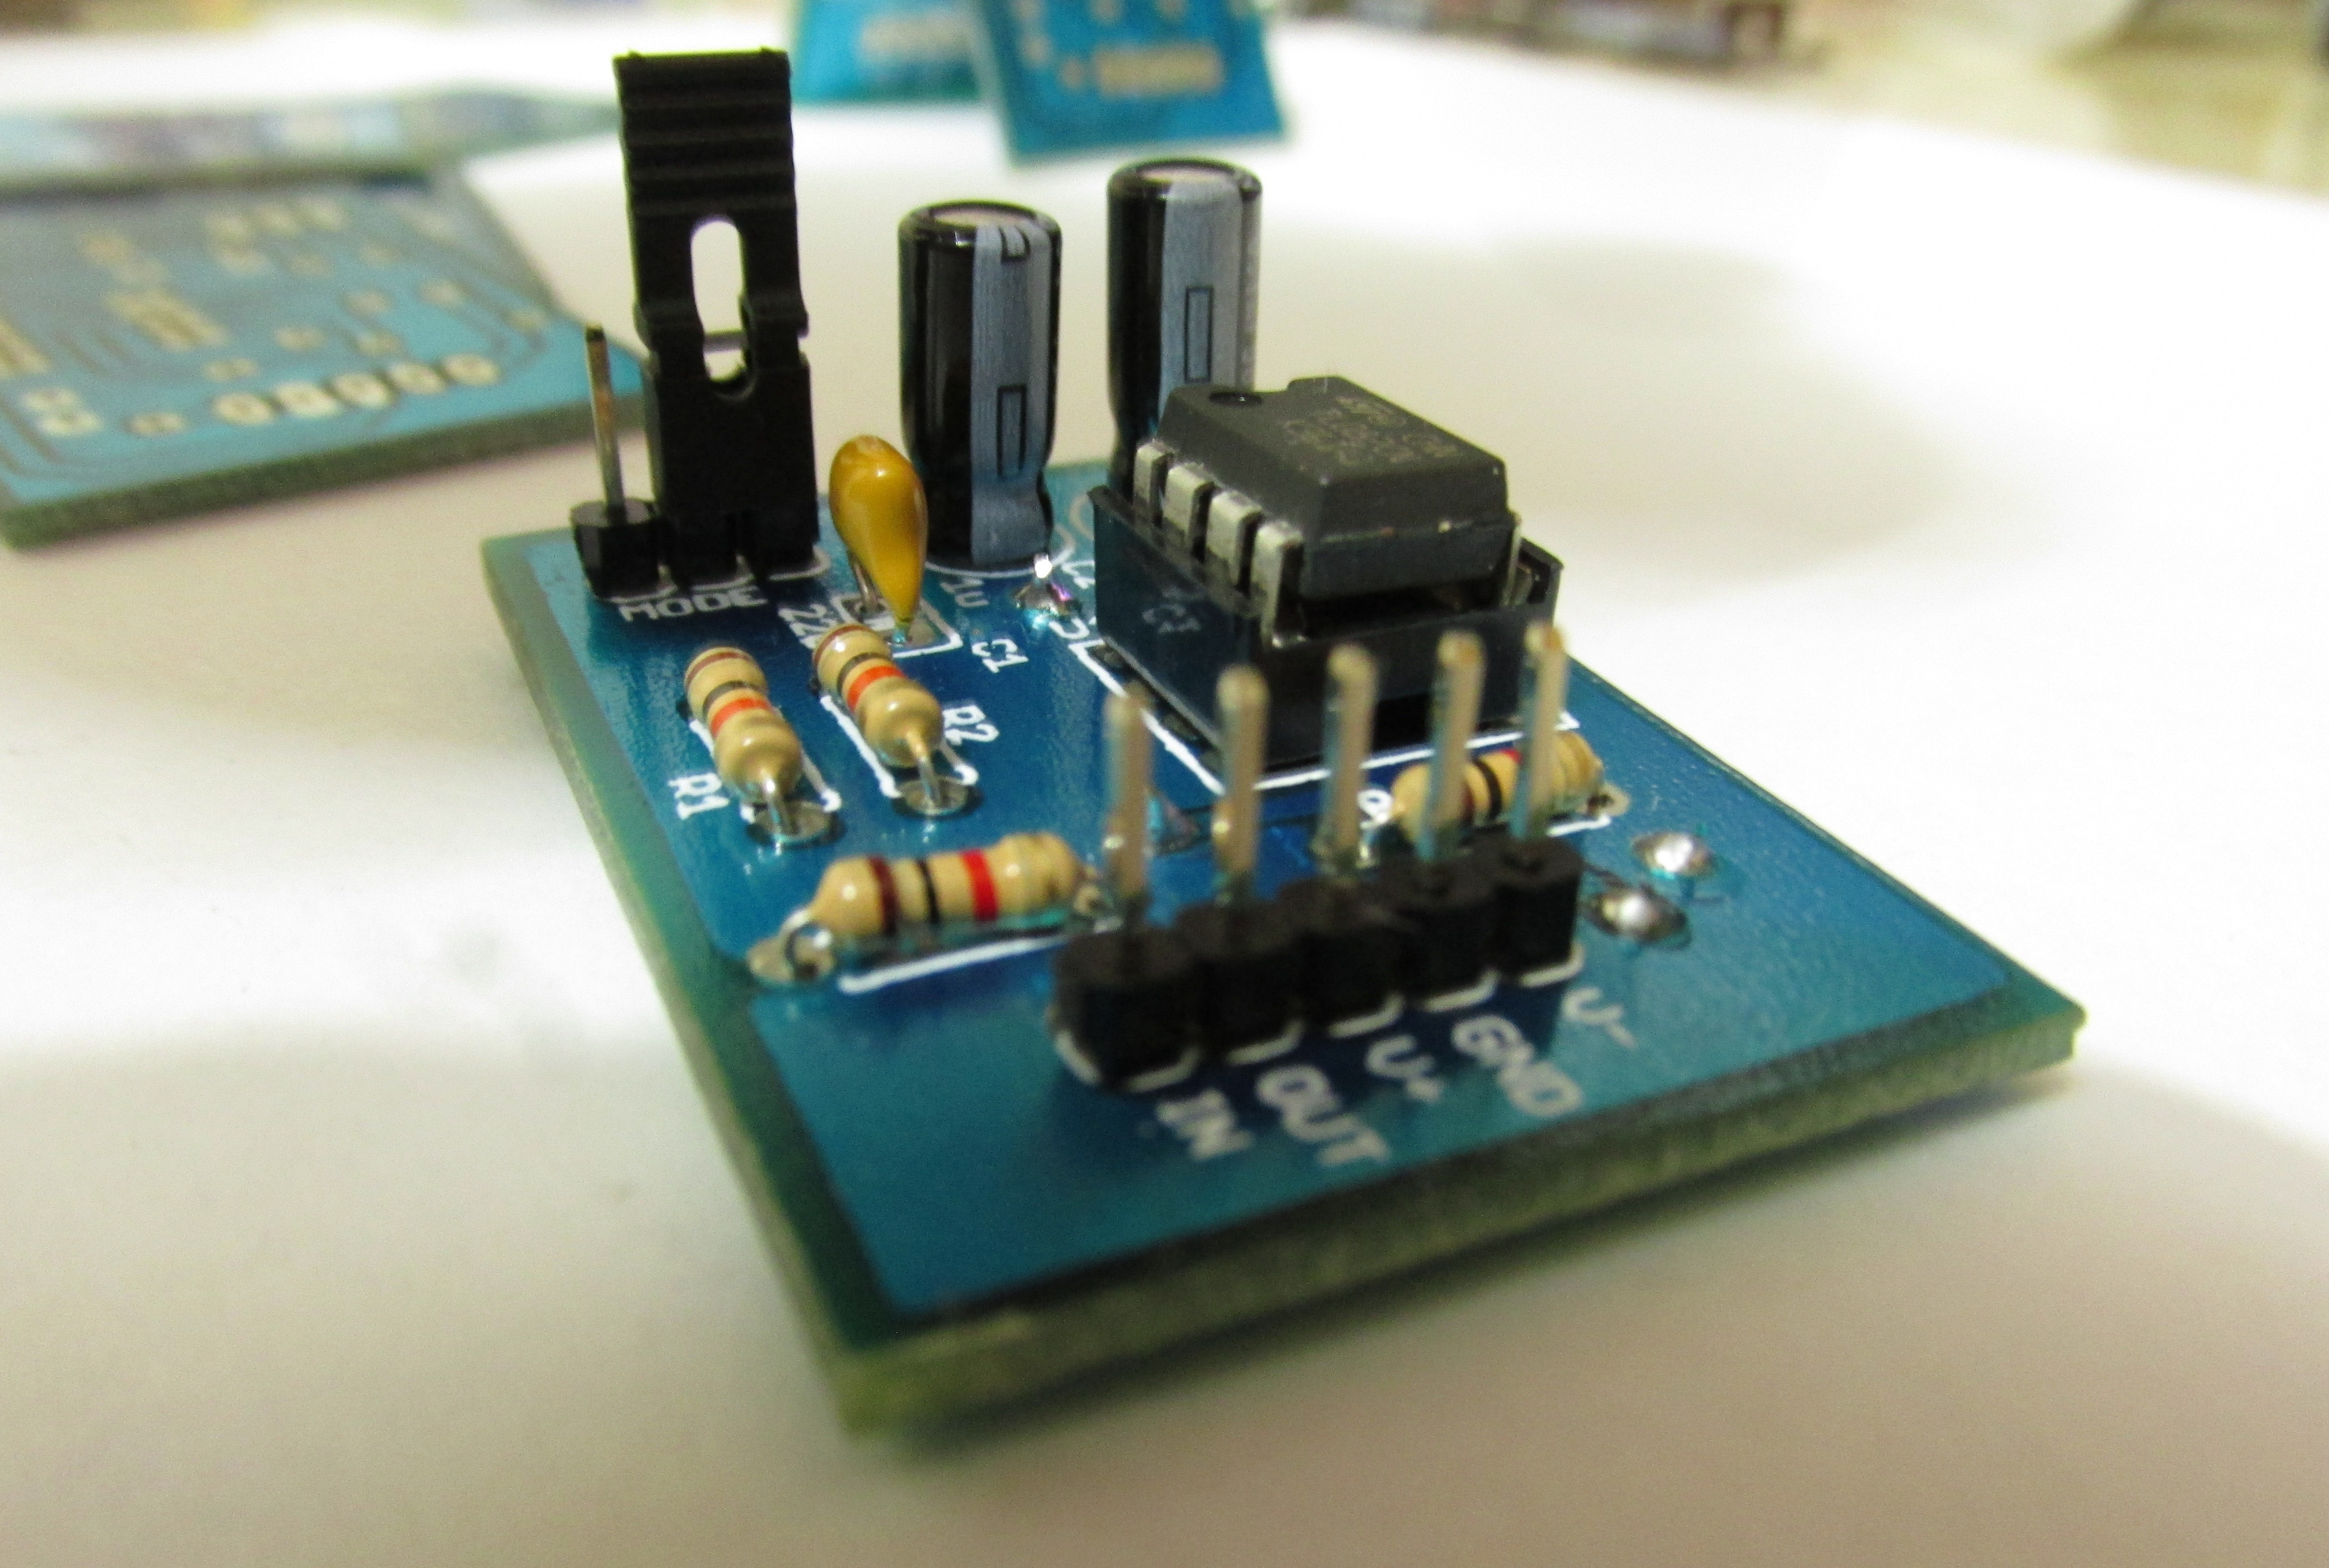
\includegraphics[scale=0.05]{images/activities/plantas_analogicas/TL082.jpg}
  \caption{PCB impreso de la planta TL082}
  \label{fig:TL082}
\end{figure}

También diseñamos una planta basada en un paper del MIT en dos modos (dos plantas). Ambas de segundo orden pero de diferente comportamiento. Una sobreamortiguada y la otra subamortiguada. Ver figuras ~\ref{fig:schematic-planta-mit}, ~\ref{fig:proteus-mit}, ~\ref{fig:board-planta-mit}, ~\ref{fig:mit-sobre} y ~\ref{fig:mit-sub}.

\begin{figure}[h!]
  \centering
  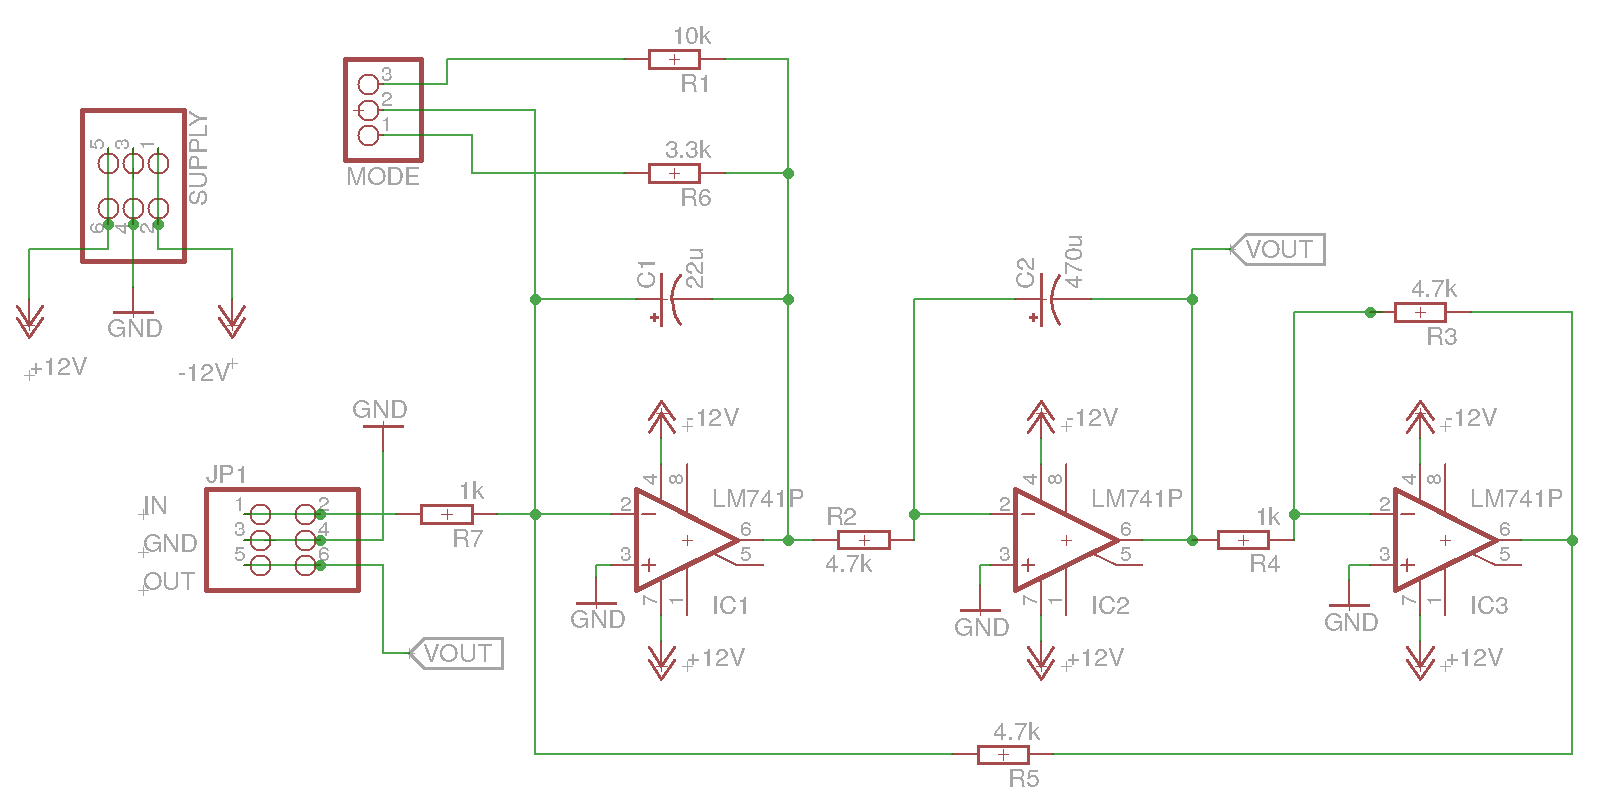
\includegraphics[scale=0.25]{images/activities/plantas_analogicas/schematic-planta-mit.png}
  \caption{Esquemático de la planta MIT}
  \label{fig:schematic-planta-mit}
\end{figure}

\begin{figure}[h!]
  \centering
  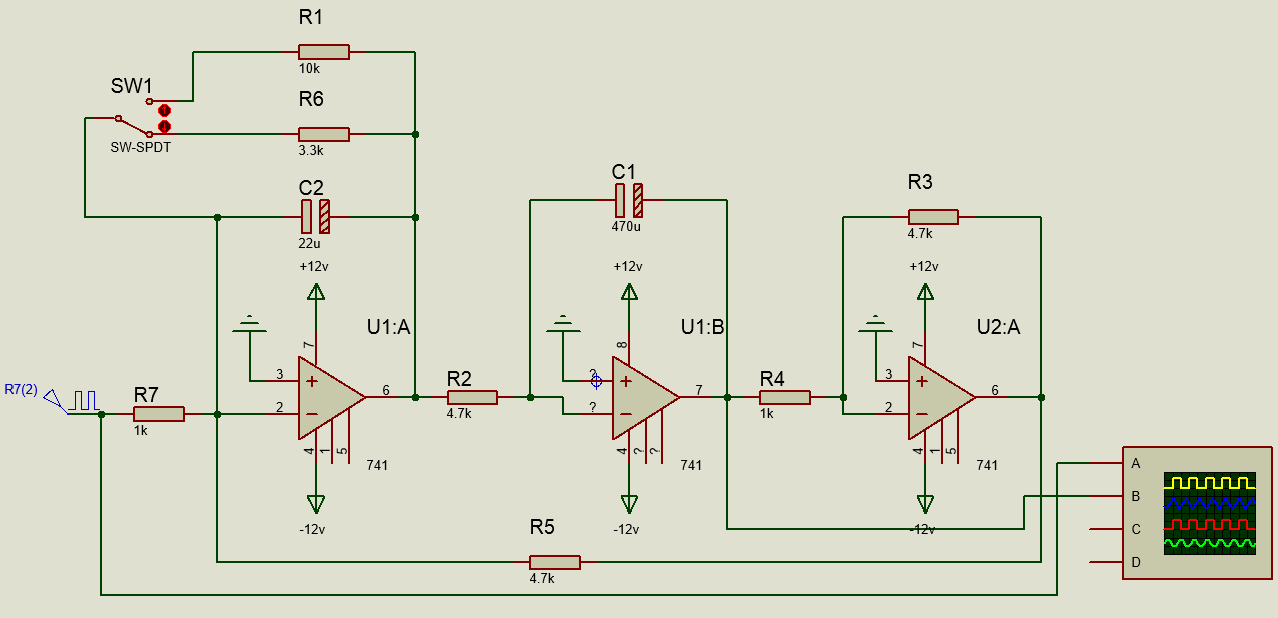
\includegraphics[scale=0.35]{images/activities/plantas_analogicas/proteus-mit.png}
  \caption{Simulaciones de la planta en Proteus}
  \label{fig:proteus-mit}
\end{figure}

\begin{figure}[h!]
  \centering
  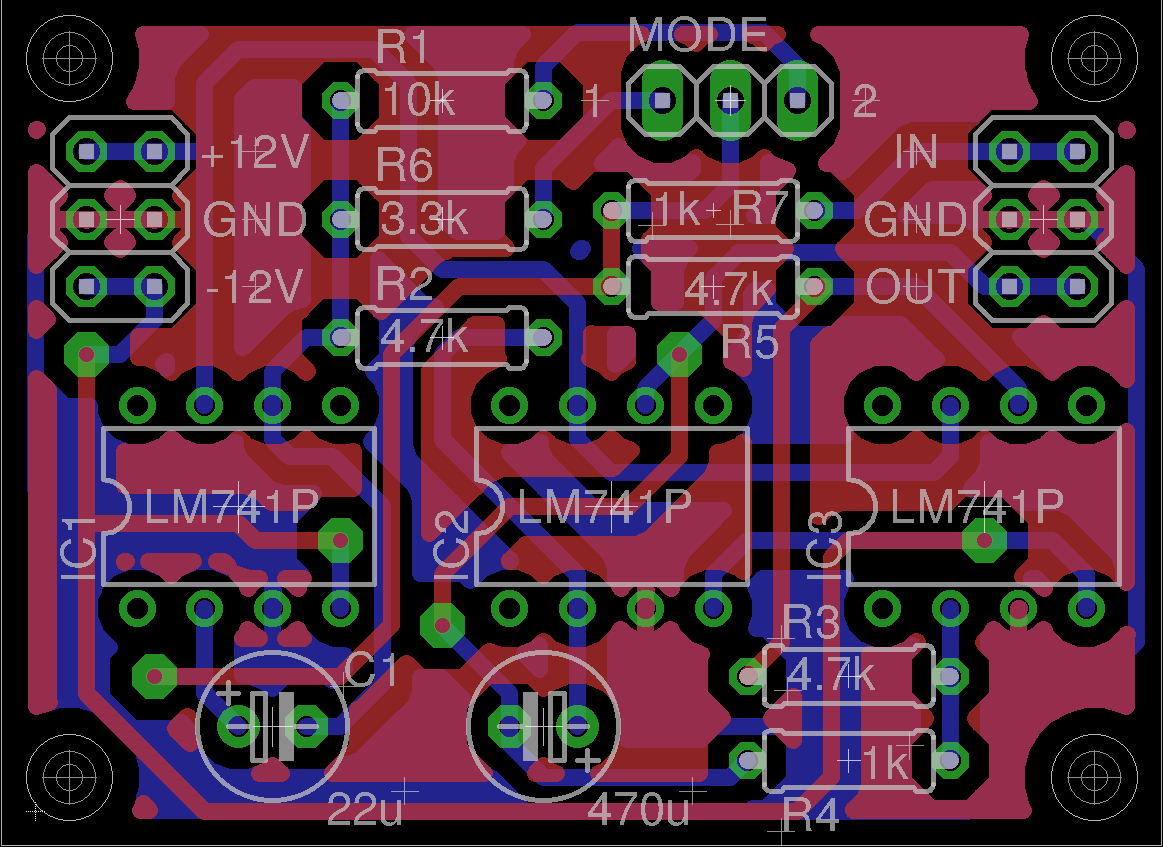
\includegraphics[scale=0.25]{images/activities/plantas_analogicas/board-planta-mit.png}
  \caption{PCB impreso de la planta MIT}
  \label{fig:board-planta-mit}
\end{figure}

\begin{figure}[h!]
  \centering
  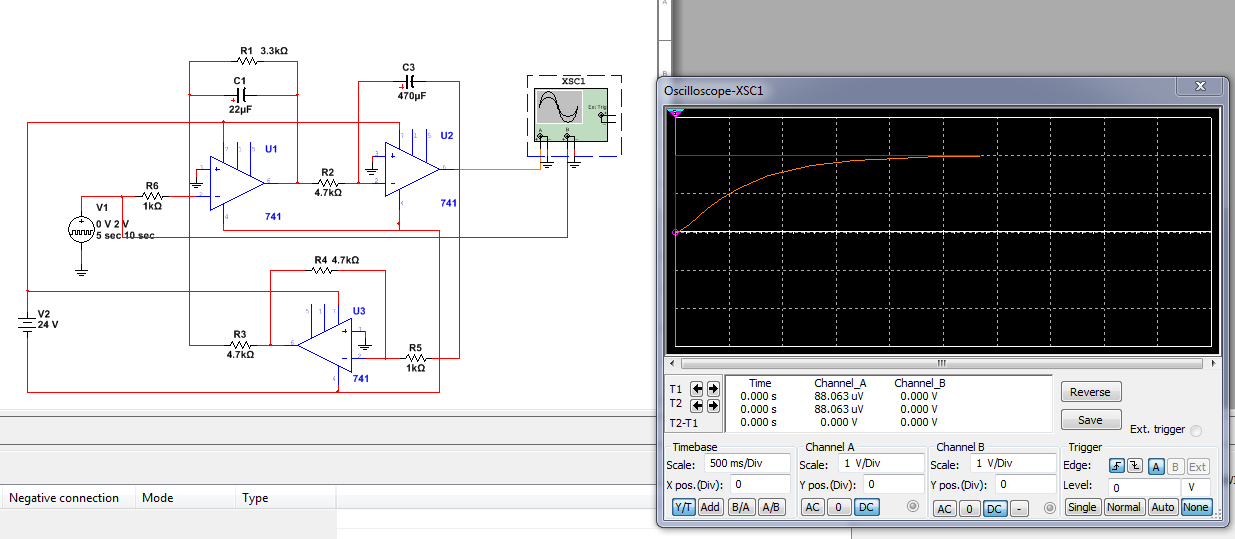
\includegraphics[scale=0.3]{images/activities/plantas_analogicas/mit-sobre.png}
  \caption{Respuesta sobreamortiguada de la planta MIT}
  \label{fig:mit-sobre}
\end{figure}

\begin{figure}[h!]
  \centering
  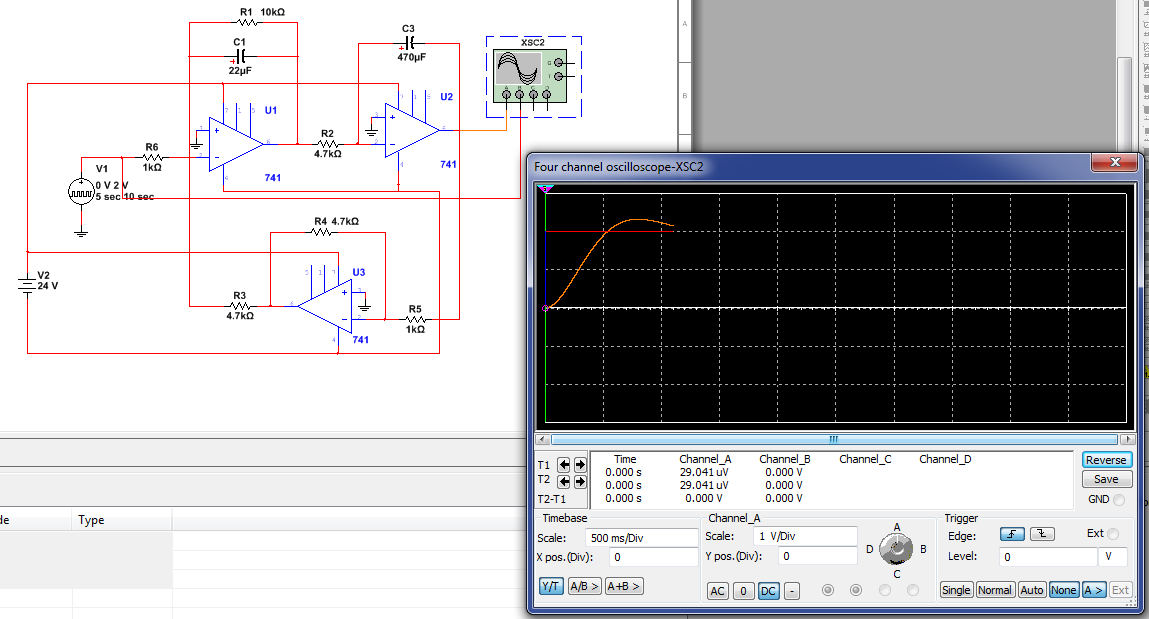
\includegraphics[scale=0.35]{images/activities/plantas_analogicas/mit-sub.png}
  \caption{Respuesta subamortiguada de la planta MIT}
  \label{fig:mit-sub}
\end{figure}

\clearpage

\subsection{Diseño e Implementación de Robot Móvil}

Durante nuestra instancia en la empresa se nos dio la libertad de desarrollar proyectos personales como este. En esta sección explico como construimos un robot móvil diferencial con el objetivo de tomar fotografías y transmitirlas en tiempo real a un web. 

Nuestro robot era controlado por una aplicación móvil desarrollada en Android, con la que le enviamos comandos al robot, este recibía y ejecutaba dichos comandos mediante un Arduino (Ver figura ~\ref{fig:arduino}).

Las fotografías eran capturadas gracias a una cámara conectada a un raspberry pi. El raspberry pi utilizado desempeñaba la tarea de servidor web, de modo que cualquier cliente conectado a la misma red podia observar las fotos que se hiban capturando en tiempo real.

\begin{figure}[h!]
  \centering
  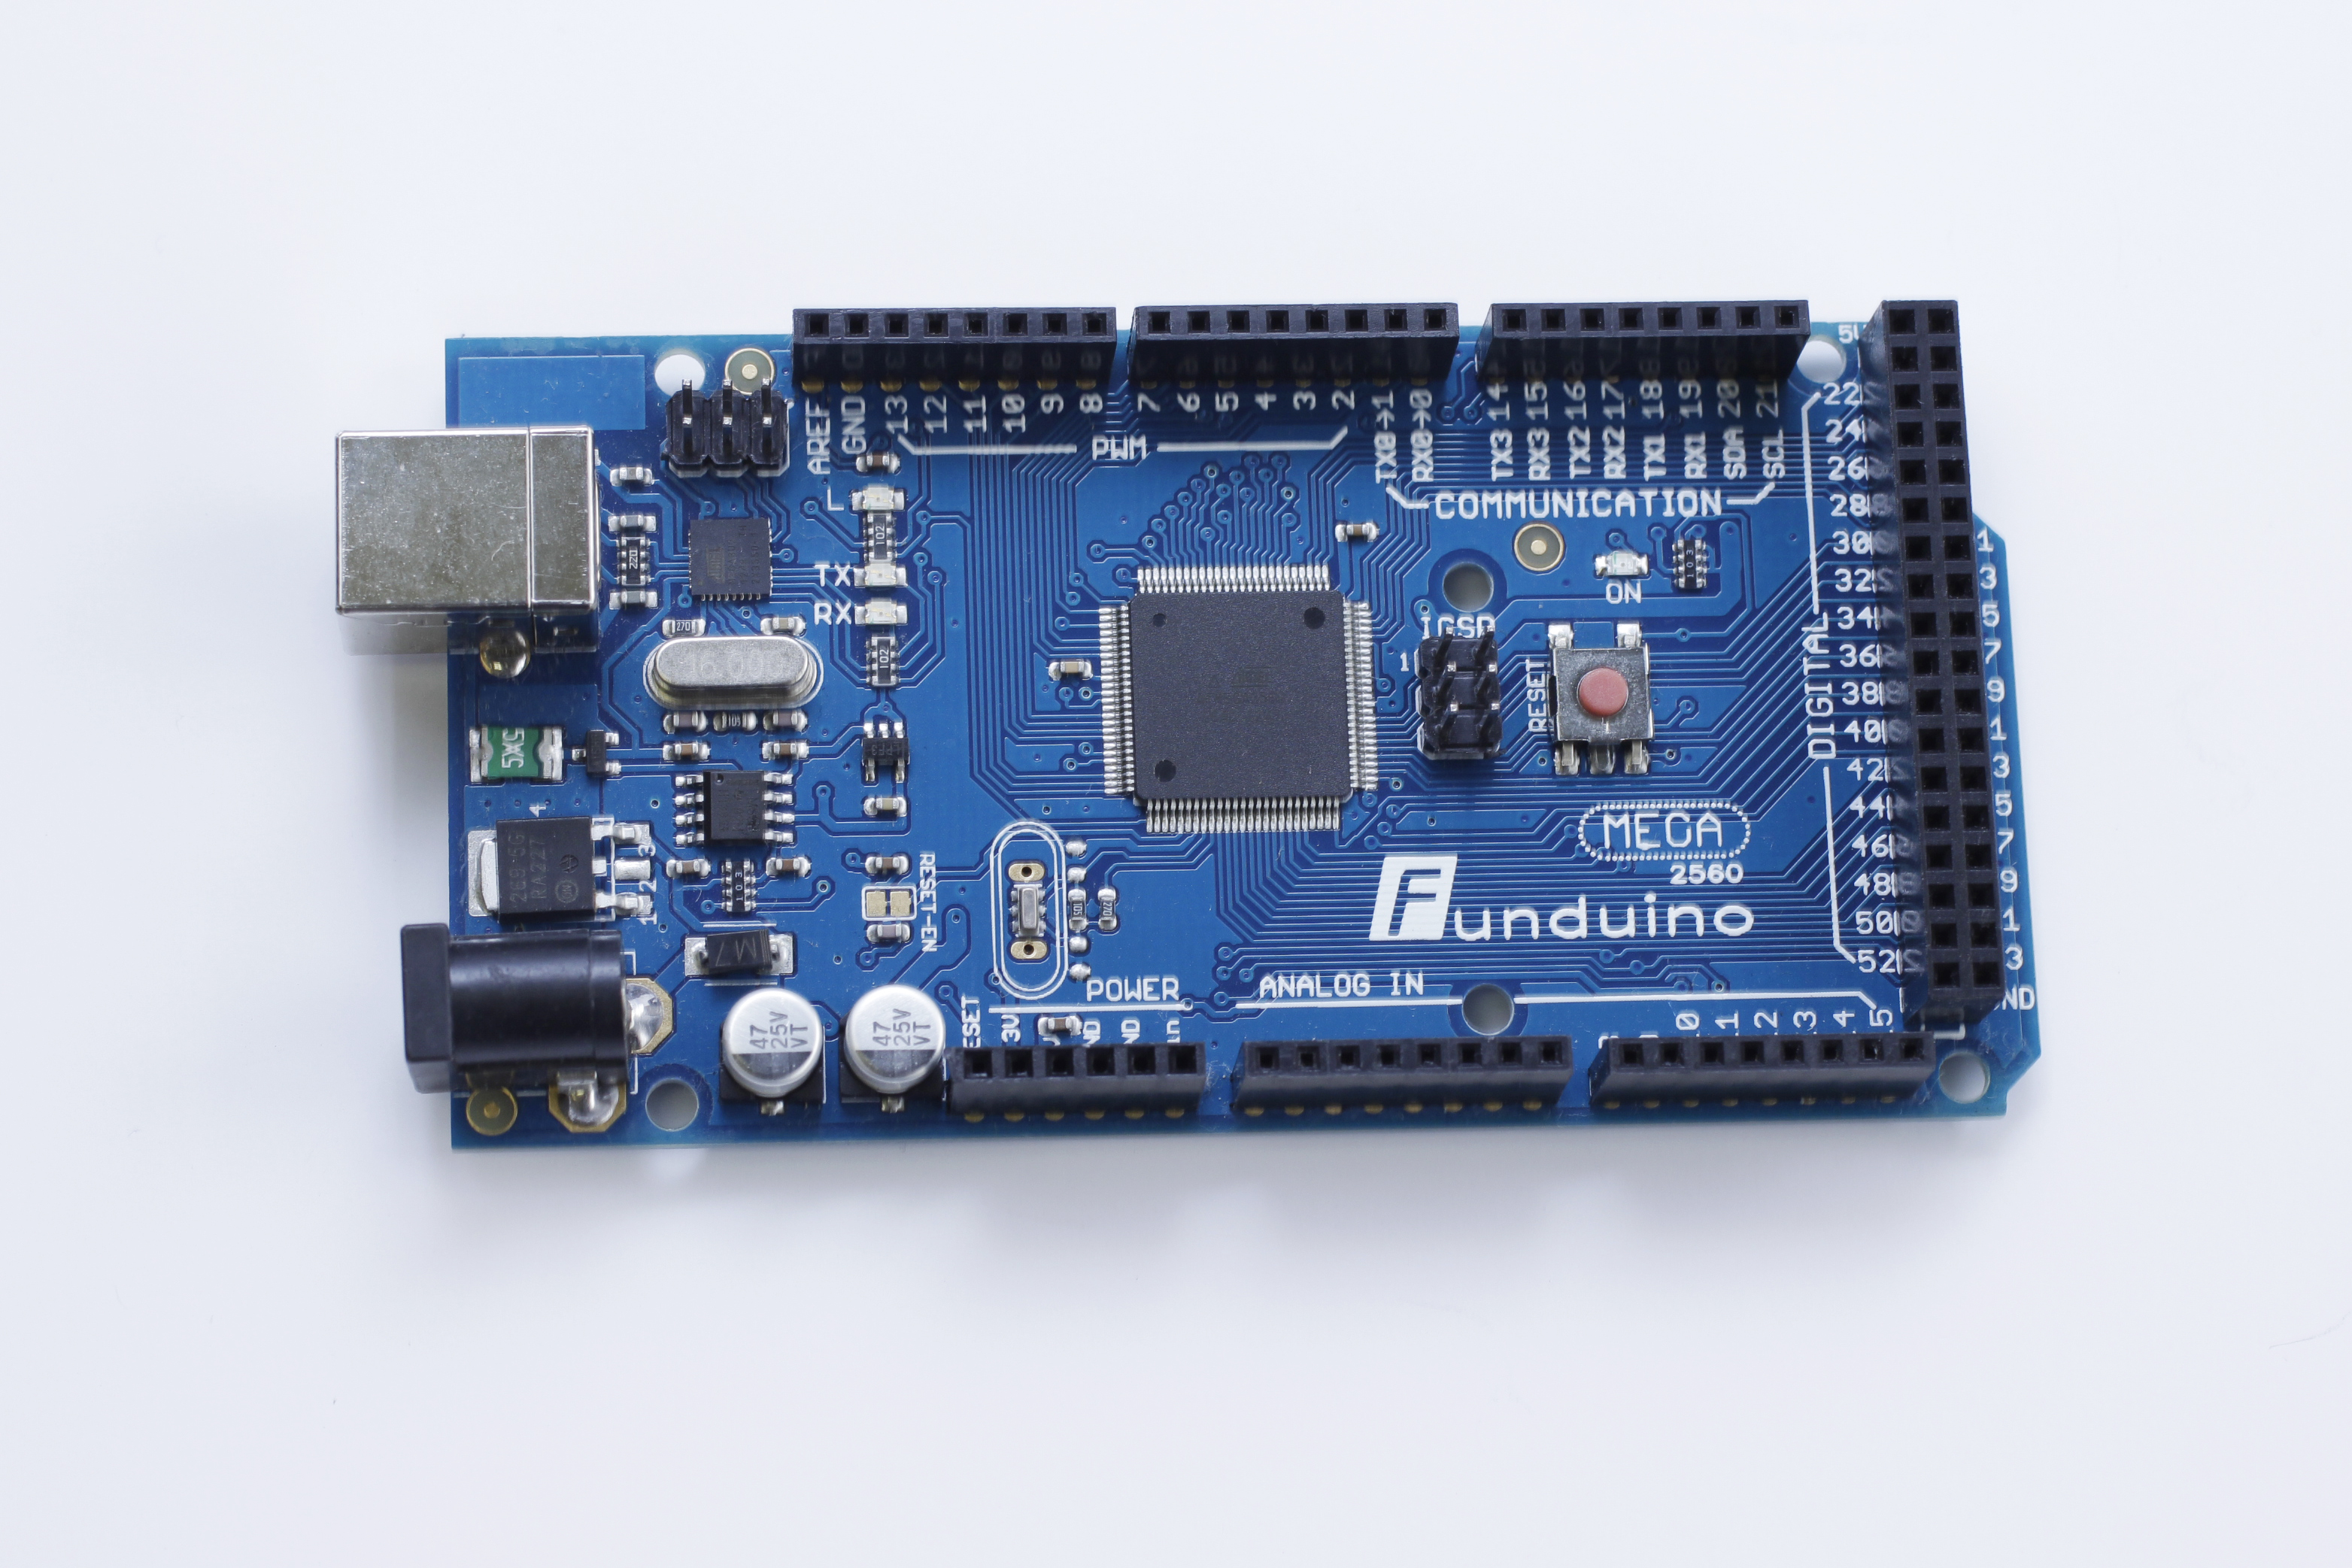
\includegraphics[scale=0.1]{images/activities/robot_movil/arduino.jpg}
  \caption{Arduino Megar 2560}
  \label{fig:arduino}
\end{figure}

\begin{figure}[h!]
  \centering
  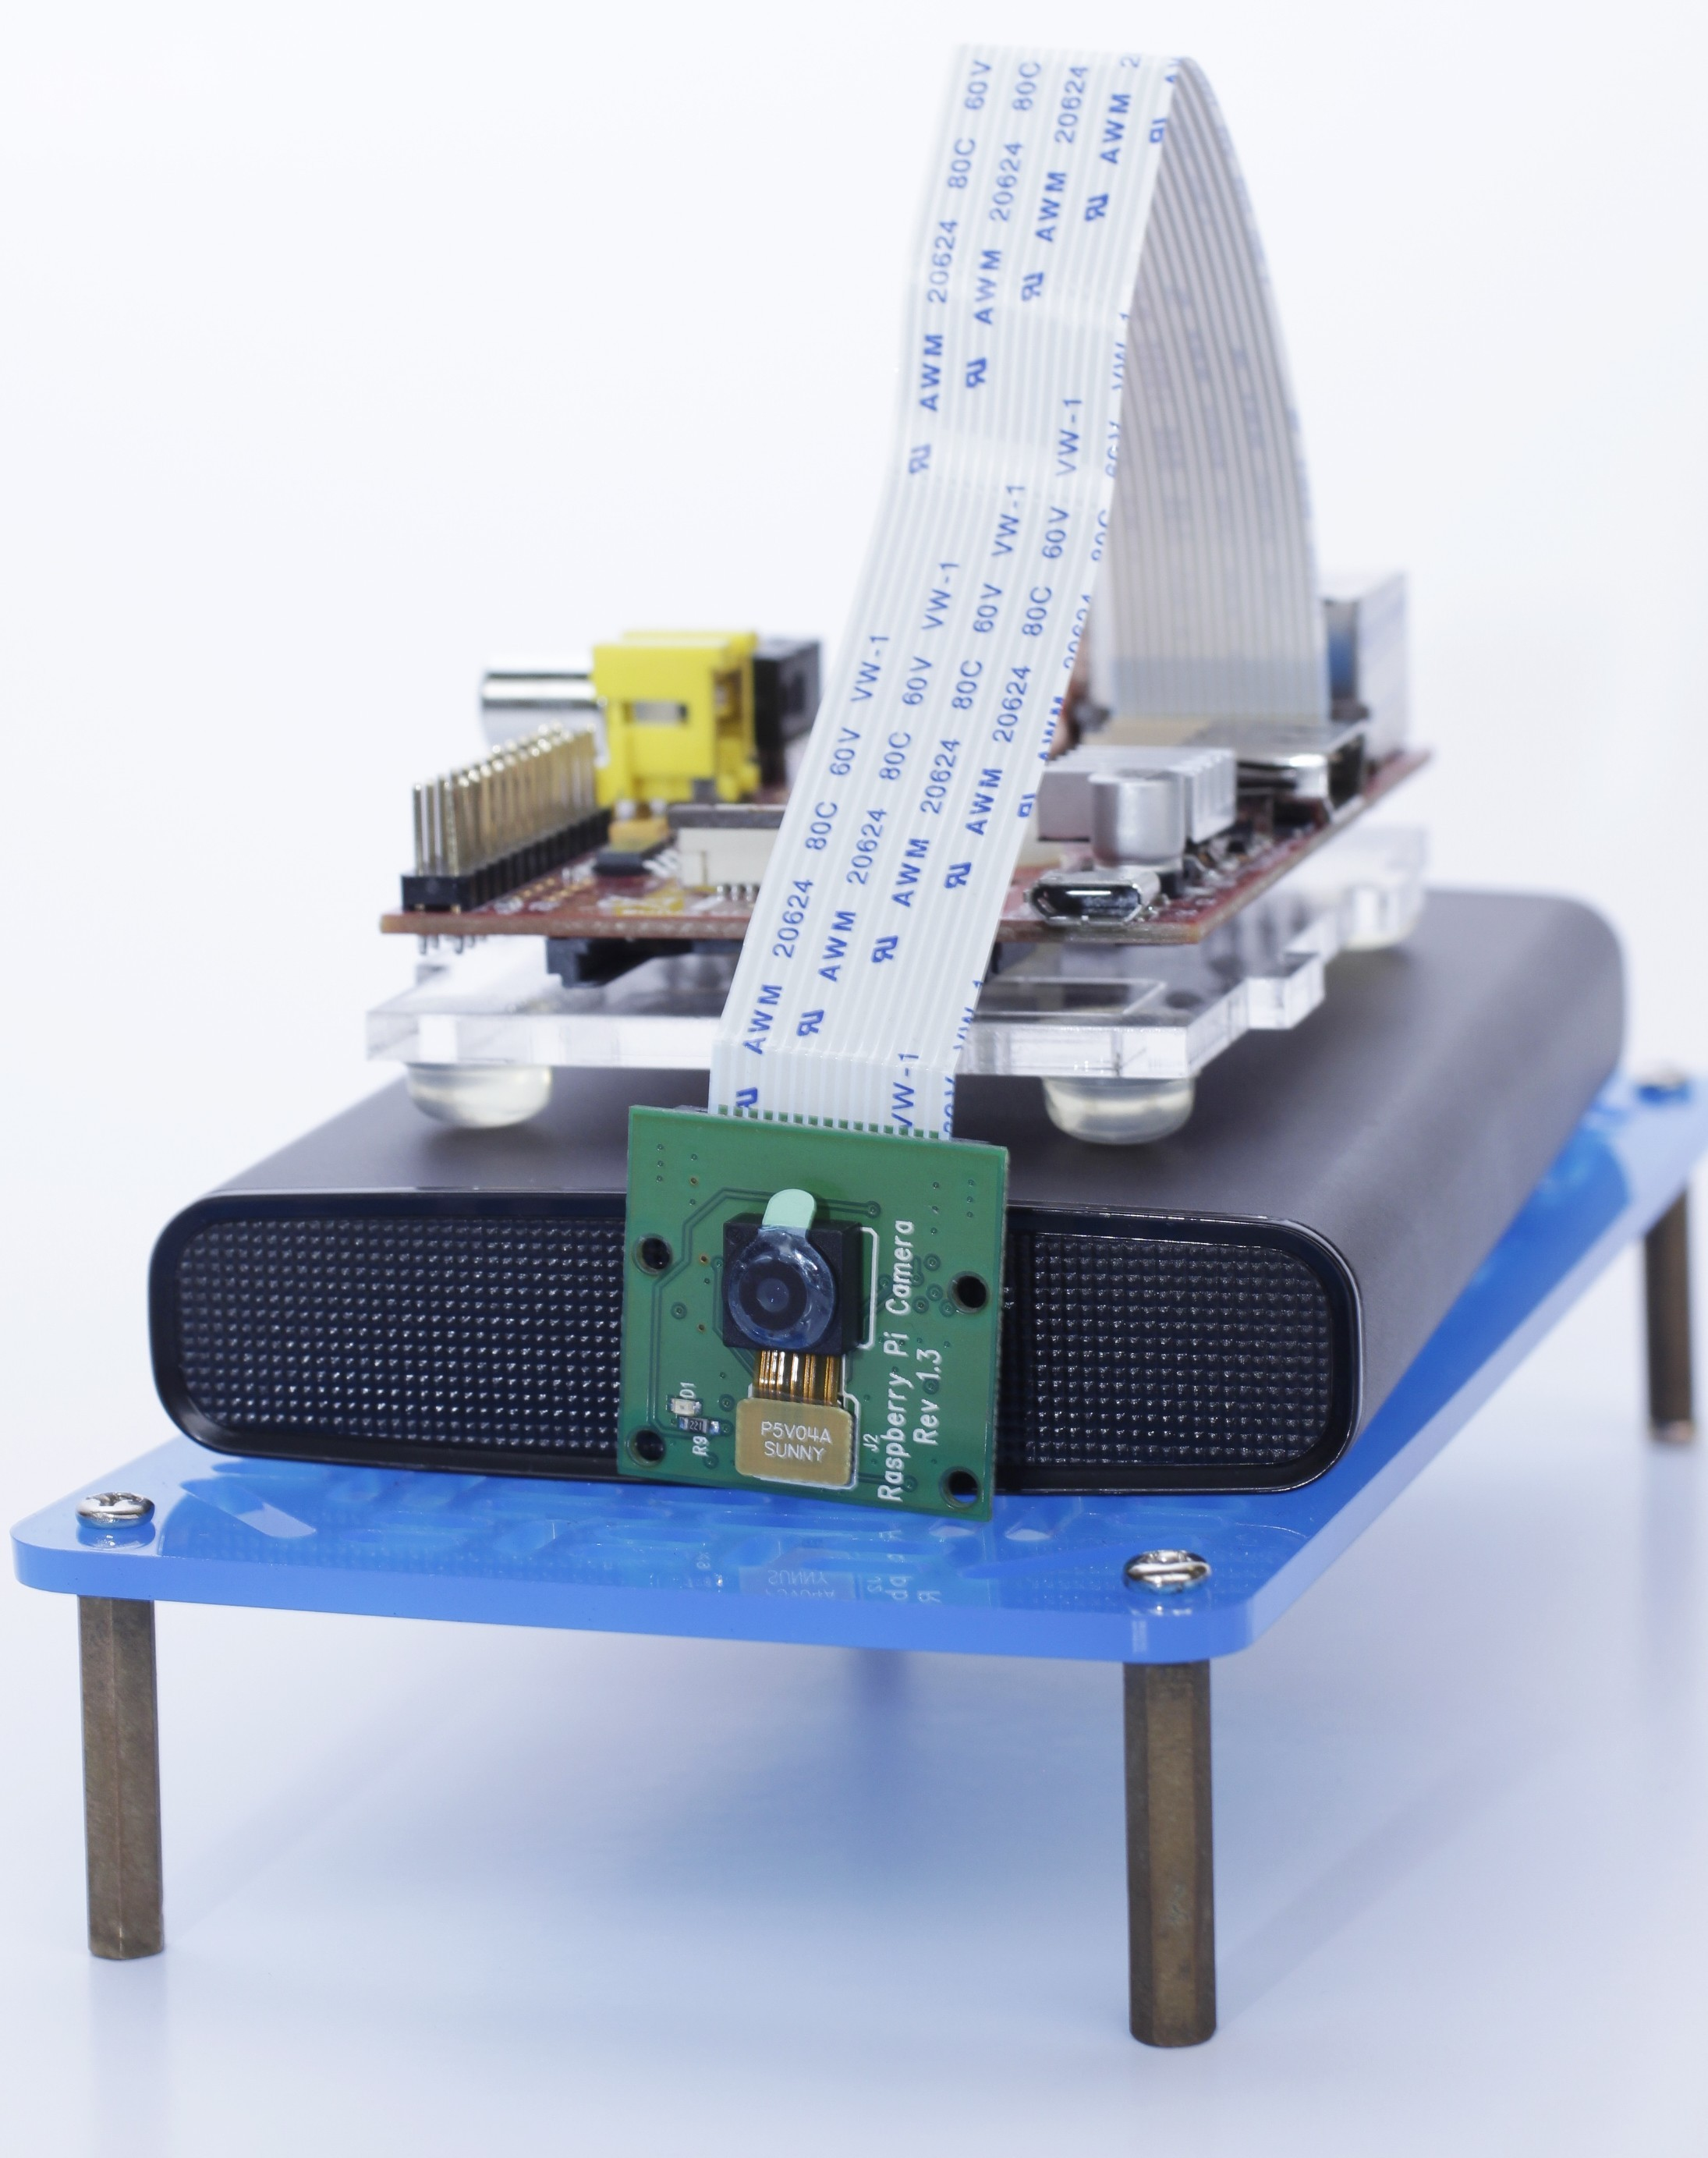
\includegraphics[scale=0.1]{images/activities/robot_movil/raspberry-pi.jpg}
  \caption{Raspberry pi, bateria y cámara}
  \label{fig:raspberry-pi}
\end{figure}

Para la comunicación del smartphone con el arduino se empleó un módulo bluetooth (hc-05). El arduino recibía los comandos, los comparaba y controlaba sus motores con ayuda de un puente H (L298). La interacción se puede apreciar en la figura ~\ref{fig:robot1}.

\begin{figure}[h!]
  \centering
  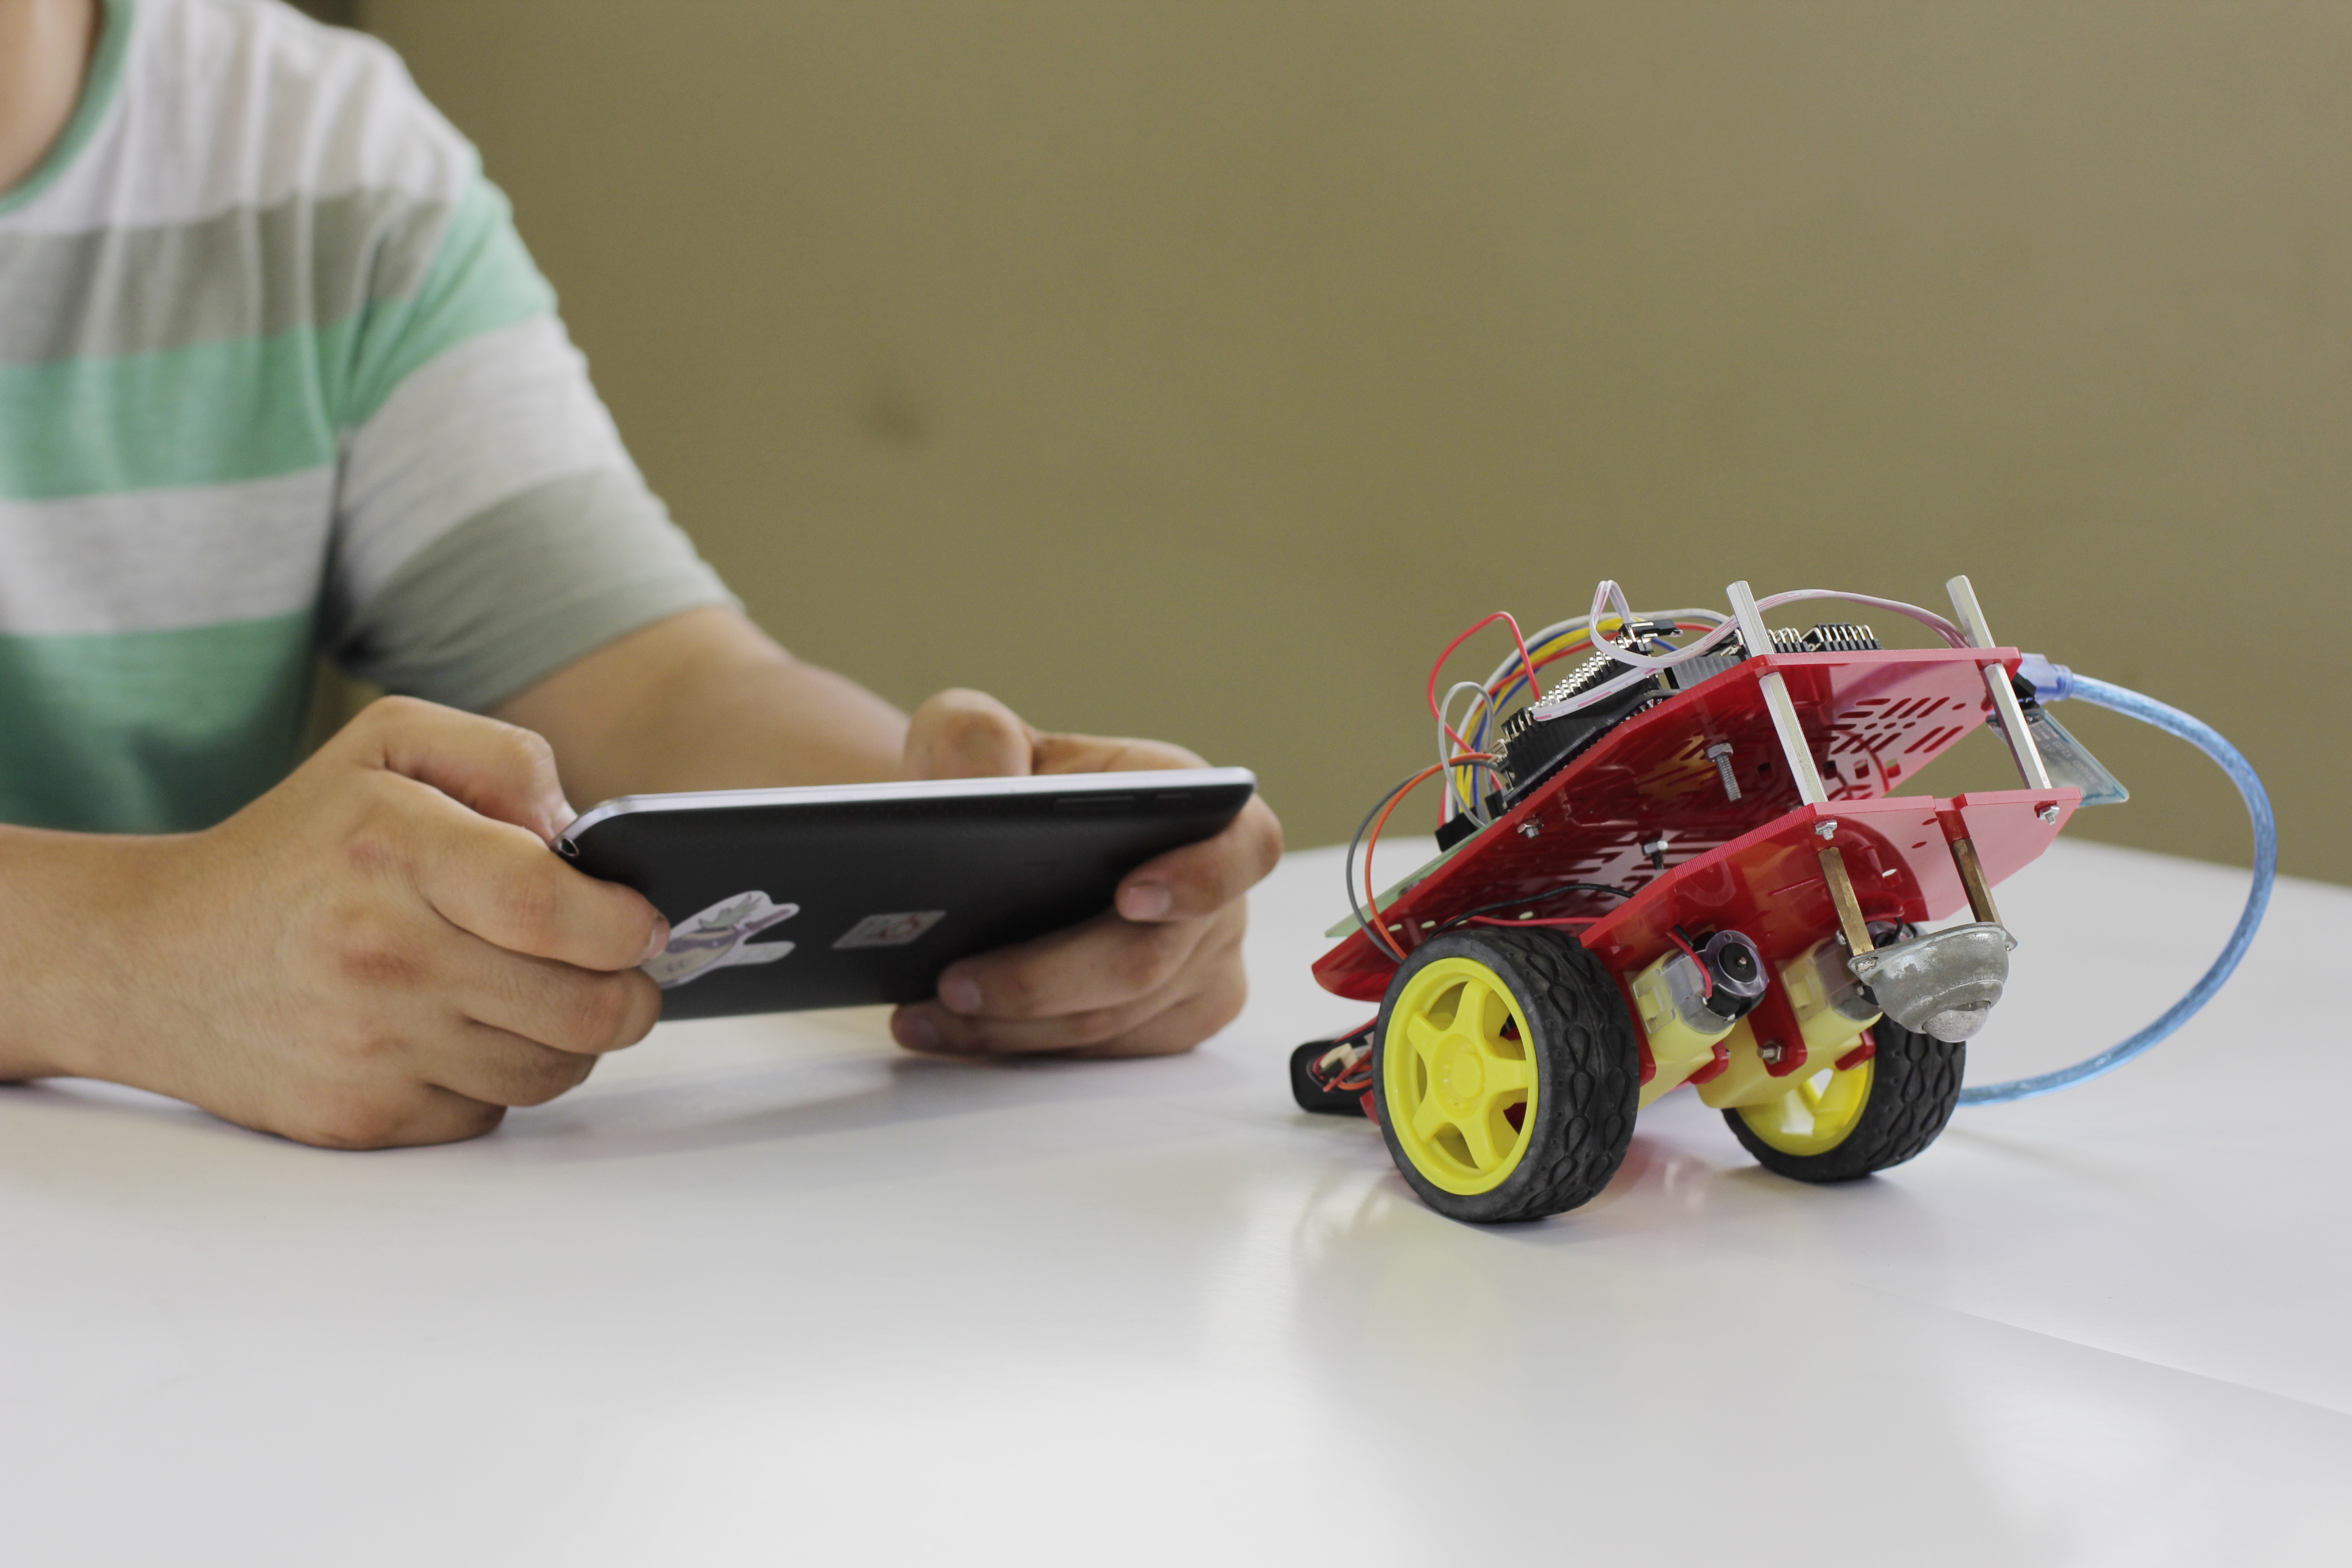
\includegraphics[scale=0.1]{images/activities/robot_movil/robot1.jpg}
  \caption{Controlando al robot móvil}
  \label{fig:robot1}
\end{figure}

Finalmente la integración de ambos módulos se puede apreciar en la figura ~\ref{fig:robot2}. Las imagenes transmitidas en tiempo real se observan en la figura ~\ref{fig:robot3}.

\begin{figure}[h!]
  \centering
  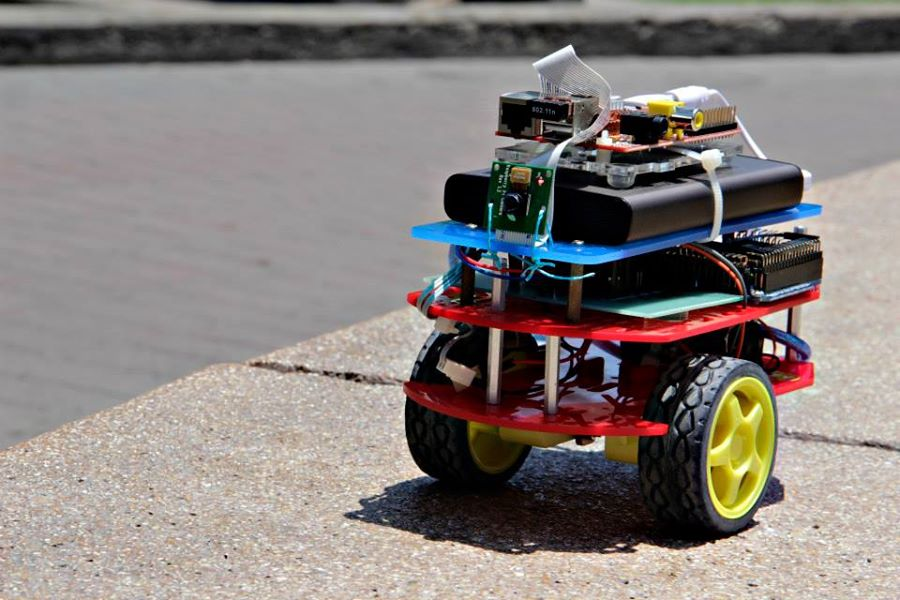
\includegraphics[scale=0.4]{images/activities/robot_movil/robot2.jpg}
  \caption{Integración del arduino como controlador y el raspberry pi como servidor}
  \label{fig:robot2}
\end{figure}

\begin{figure}[h!]
  \centering
  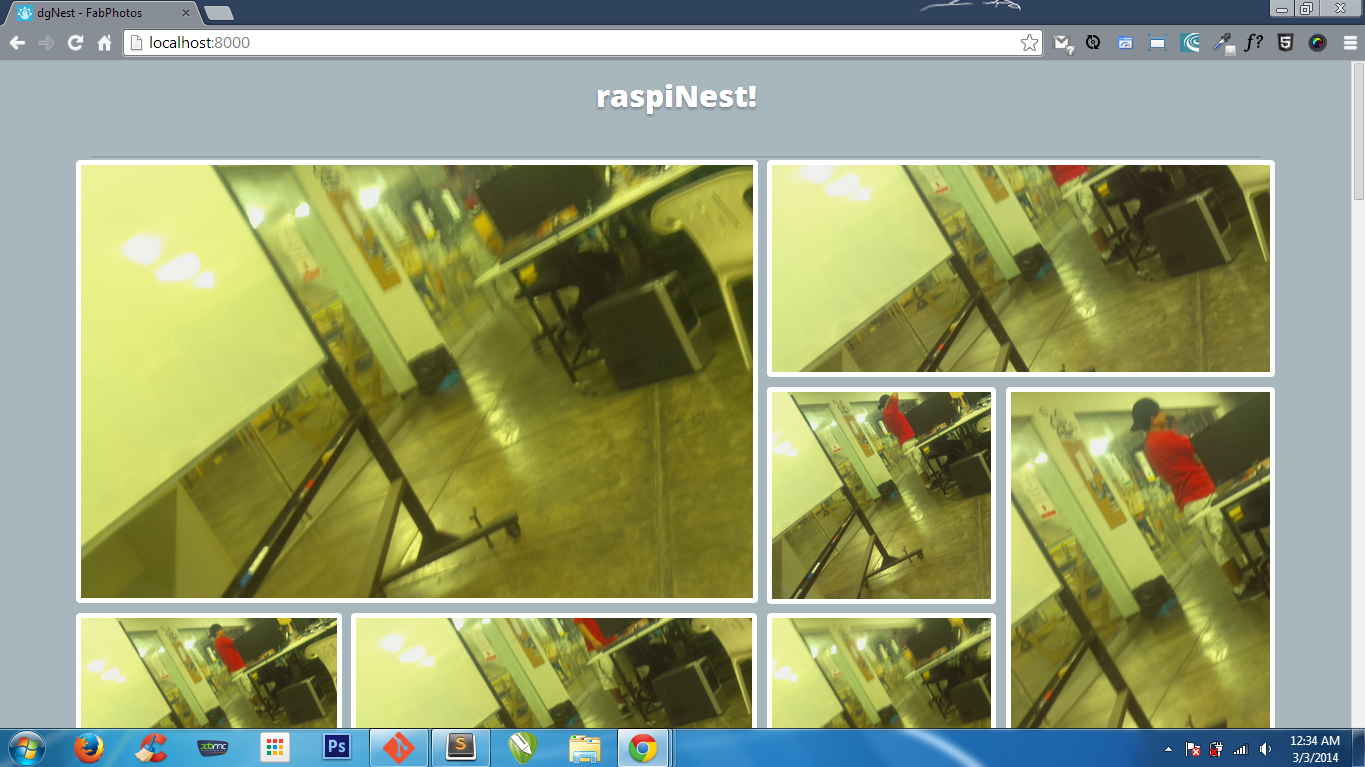
\includegraphics[scale=0.4]{images/activities/robot_movil/robot3.png}
  \caption{Aplicación web mostrando imágenes capturadas}
  \label{fig:robot3}
\end{figure}

\clearpage

\subsection{Implementación de modulos I/O DAQ}

Se implementó tarjetas que redundan los pines de la DAQ con la finalidad de facilitar su uso. El esquemático de este módulo se presenta en la figura ~\ref{fig:schematic-daq}, el board del PCB en la figura ~\ref{fig:board-daq} y el módulo final montado en la DAQ en la figura ~\ref{fig:modulo-daq}. 

\begin{figure}[h!]
  \centering
  \begin{subfigure}{0.4\textwidth}
    \centering
    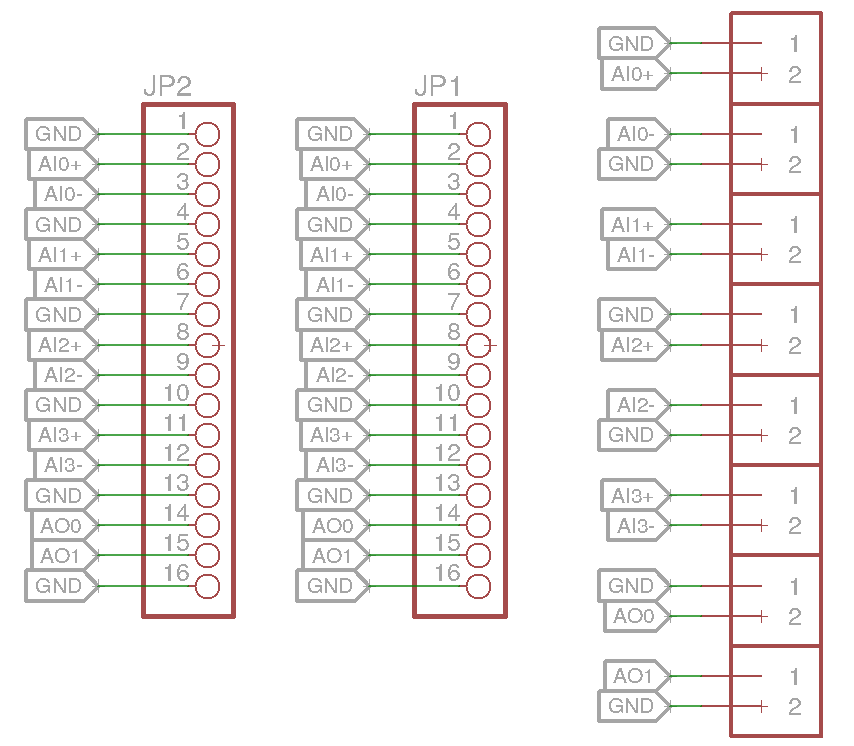
\includegraphics[width=0.9\textwidth]{images/activities/daq/schematic-daq-left.png}
    \caption{Esquemático. Lado izquierdo}
    \label{fig:schematic-daq-left}
  \end{subfigure}
  \begin{subfigure}{0.4\textwidth}
    \centering
    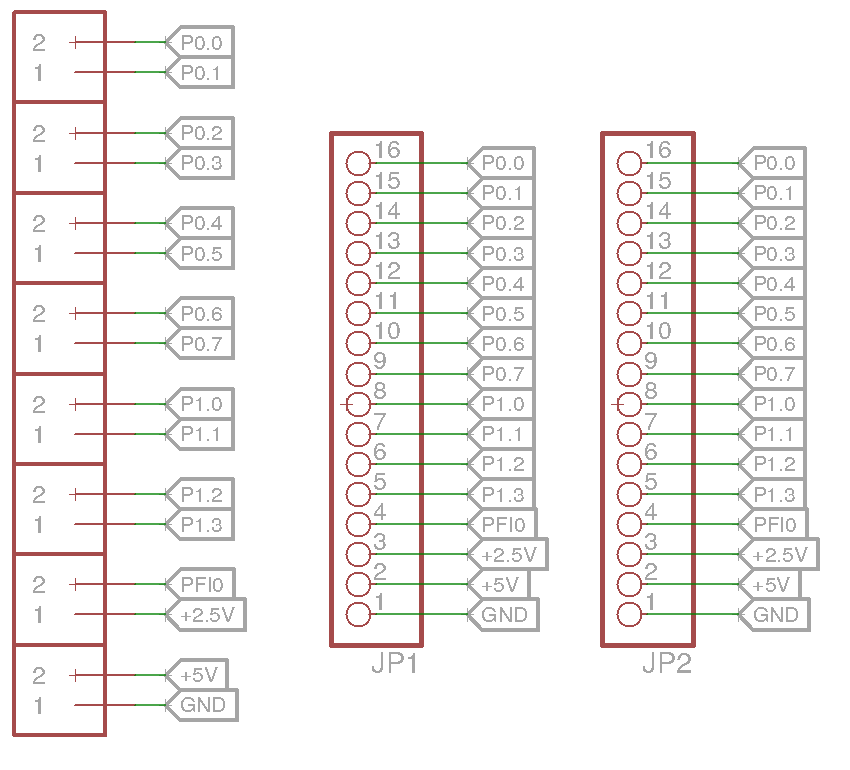
\includegraphics[width=0.9\textwidth]{images/activities/daq/schematic-daq-right.png}
    \caption{Esquemático. Lado derecho}
    \label{fig:schematic-daq-right}
  \end{subfigure}
  \caption{Esquemático DAQ}
  \label{fig:schematic-daq}
\end{figure}

\begin{figure}[h!]
  \centering
  \begin{subfigure}{0.4\textwidth}
    \centering
    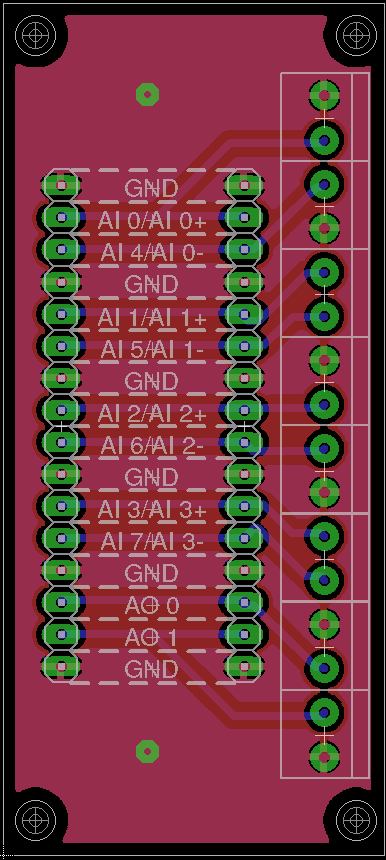
\includegraphics[width=0.6\textwidth]{images/activities/daq/board-daq-left.png}
    \caption{Board. Lado izquierdo}
    \label{fig:board-daq-left}
  \end{subfigure}
  \hfill
  \begin{subfigure}{0.4\textwidth}
    \centering
    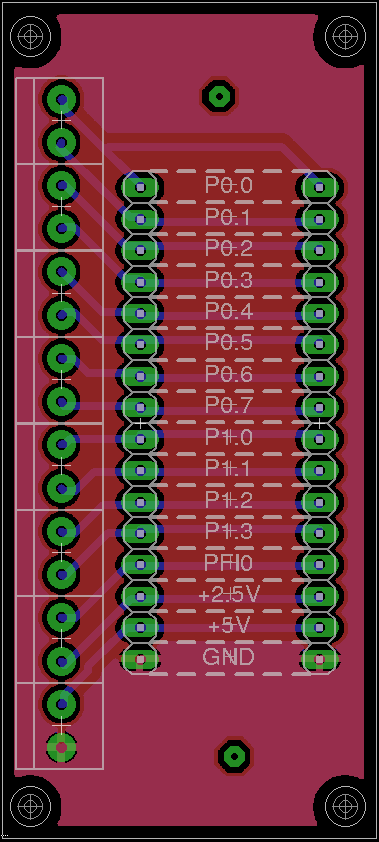
\includegraphics[width=0.6\textwidth]{images/activities/daq/board-daq-right.png}
    \caption{Board. Lado derecho}
    \label{fig:board-daq-right}
  \end{subfigure}
  \caption{Board DAQ}
  \label{fig:board-daq}
\end{figure}

\begin{figure}[h!]
  \centering
  \begin{subfigure}{0.4\textwidth}
    \centering
    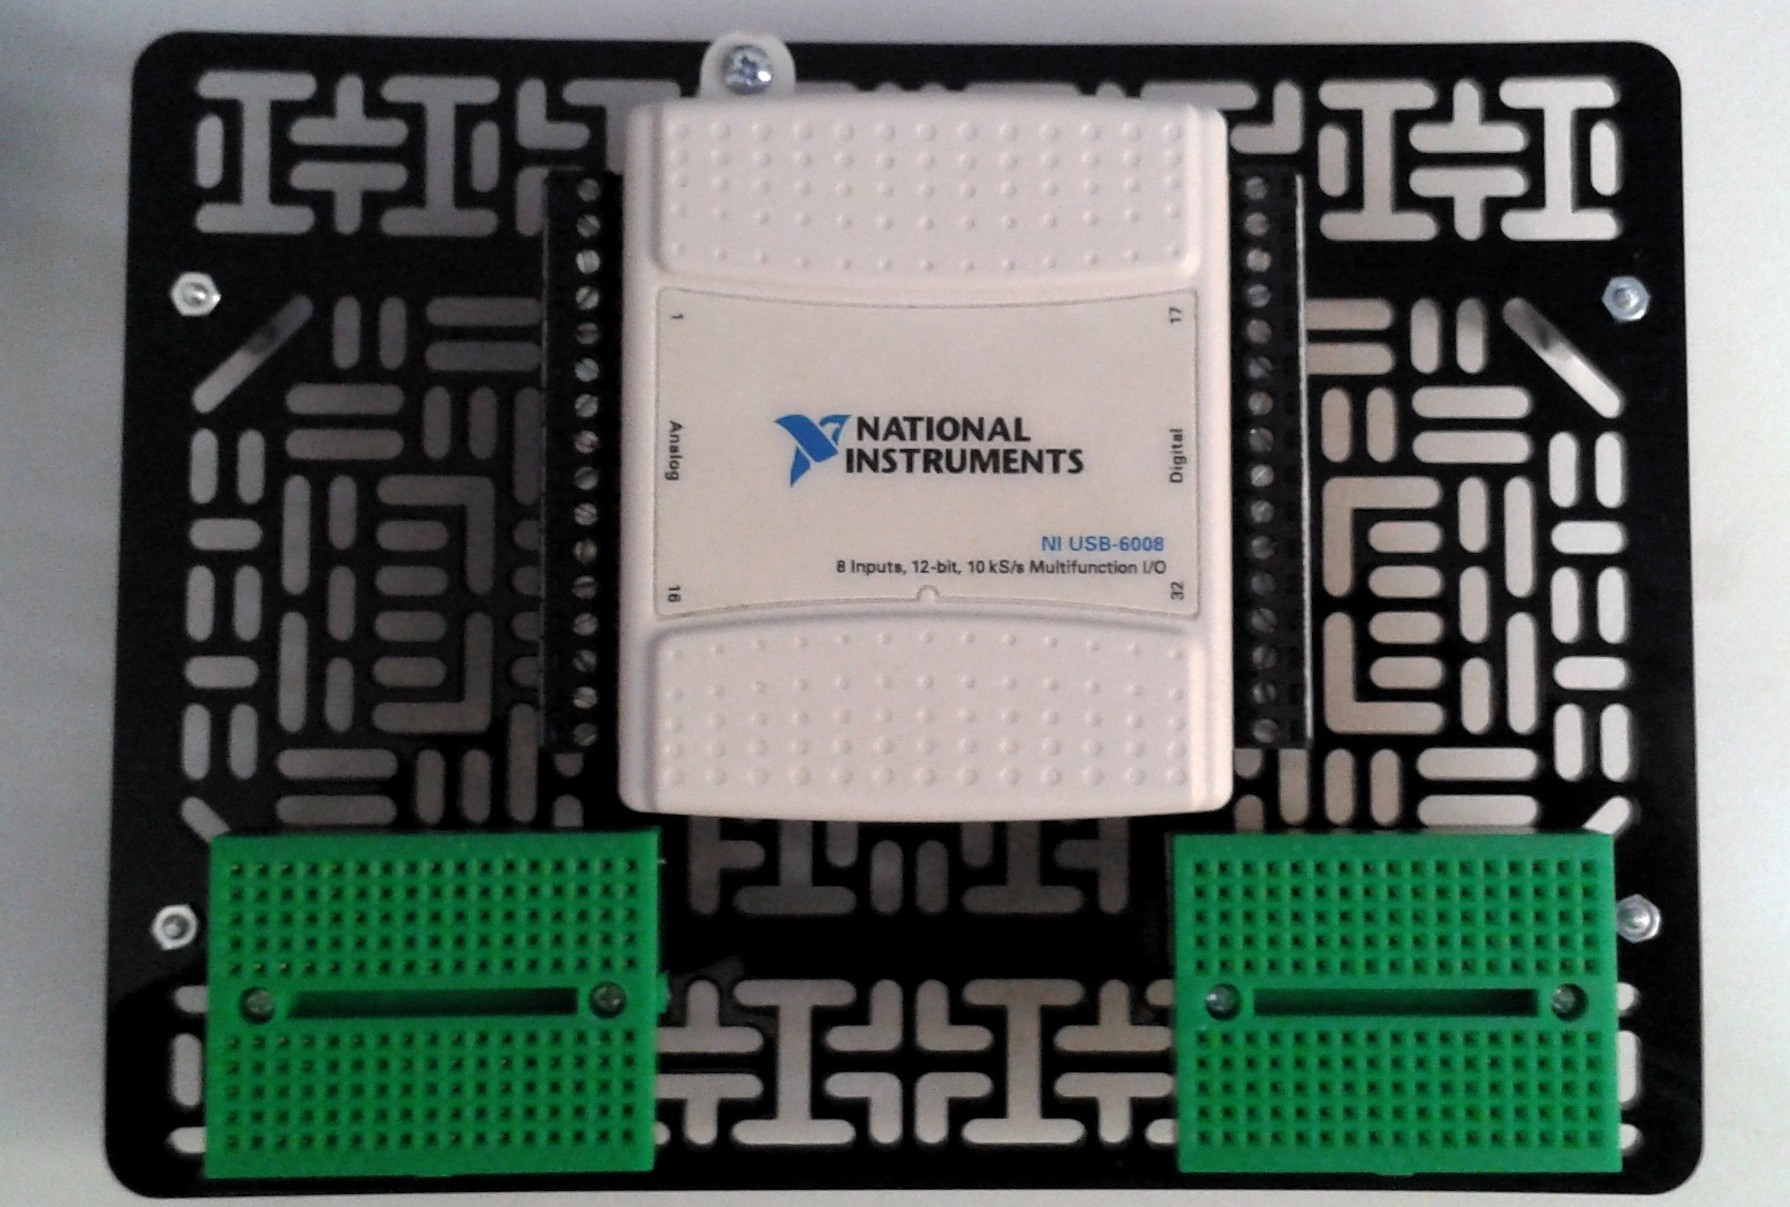
\includegraphics[width=1.2\textwidth]{images/activities/daq/daq3.jpg}
    \caption{Módulo sin las tarjetas}
    \label{fig:modulo-daq-1}
  \end{subfigure}
  \hfill
  \begin{subfigure}{0.4\textwidth}
    \centering
    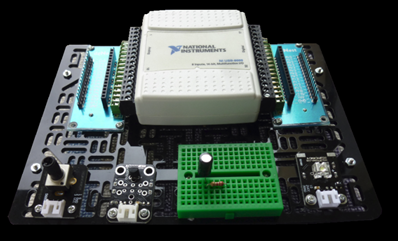
\includegraphics[width=1.2\textwidth]{images/activities/daq/daq4.png}
    \caption{Módulo con las tarjetas}
    \label{fig:modulo-daq-2}
  \end{subfigure}
  \caption{Módulo terminado}
  \label{fig:modulo-daq}
\end{figure}

\clearpage

\subsection{Diseño e Implementación de un Módulo de Entrenamiento de Redes Neuronales}

En este proyecto se implementaron módulos de entrenamiento de redes neuronales (RNA) con el fin de facilitar la electrónica que demanda esta práctica. El módulo consistia de combinaciones de compuertas lógicas, un display de siete segmentos y tiras de leds; las cuales son empleadas como parte del entrenamiento de la red y como salidas de este. Ver figuras ~\ref{fig:esquematico-rna} y ~\ref{fig:board-rna}.

\begin{figure}[h!]
  \centering
  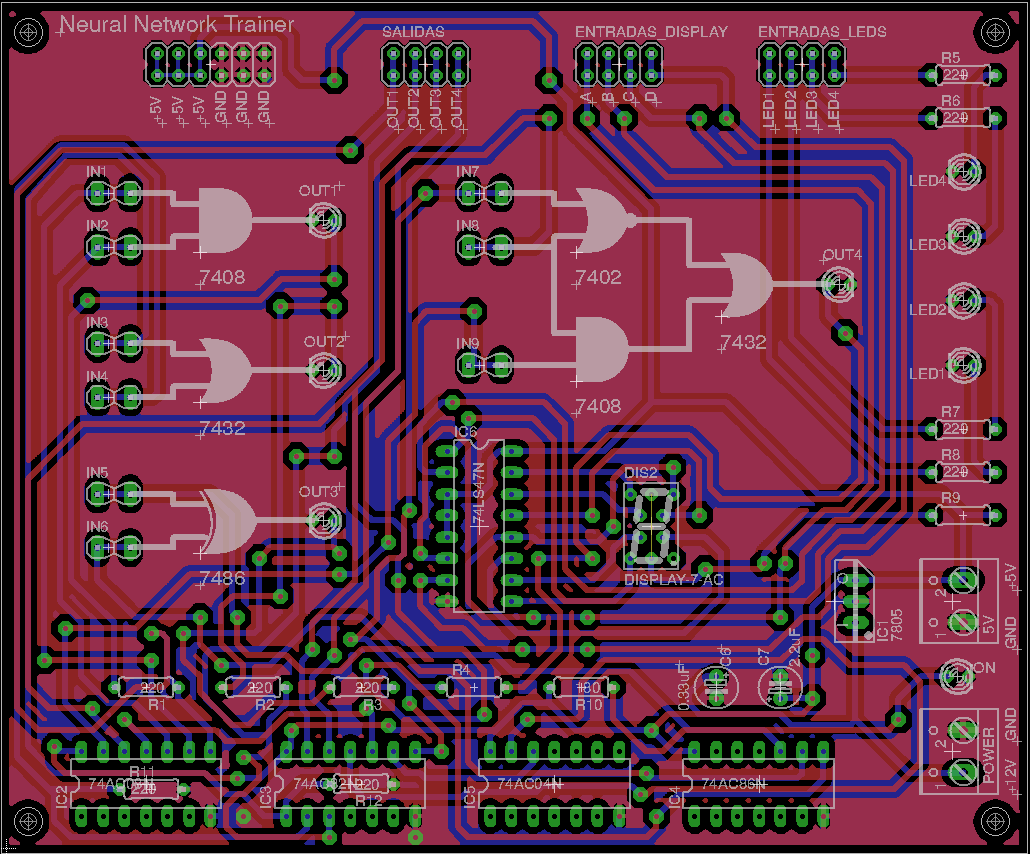
\includegraphics[scale=0.36]{images/activities/modulo_rna/rna1.png}
  \caption{Esquemático del módulo RNA}
  \label{fig:esquematico-rna}
\end{figure}

\begin{sidewaysfigure}[h!]
  \centering
  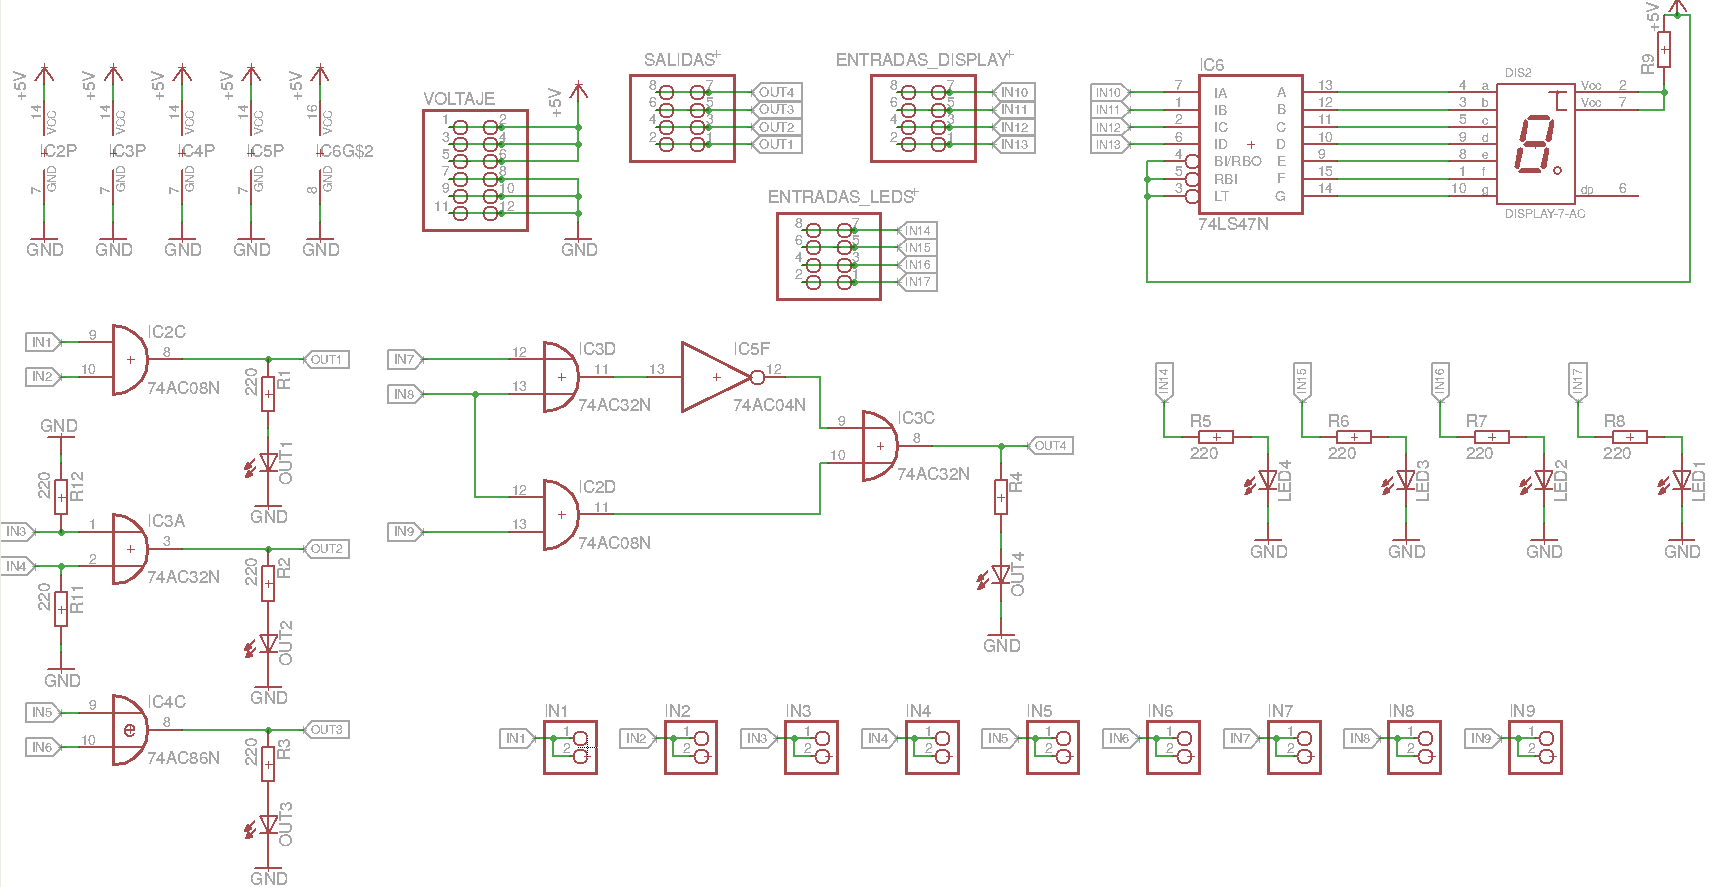
\includegraphics[scale=0.3]{images/activities/modulo_rna/rna2.png}
  \caption{PCB board del módulo RNA}
  \label{fig:board-rna}
\end{sidewaysfigure}

\clearpage

\subsection{Implementación de conversor RJ11 a ICSP}

Se desarrolló un conversor RJ11 a ICSP de bajo costo, el cual es empleado con el módulo pickit 3 para grabar un DSPIC. El diseño del board se observa en la figura ~\ref{fig:board-dspic}. El circuito original de fábrica se muestra en la figura ~\ref{fig:original-dspic} y los módulos terminados en la figura ~\ref{fig:modulos-dspic}.

\begin{figure}[h!]
  \centering
  \includegraphics[scale=0.36]{images/activities/adaptador_rj11_icsp/board-rj11-icsp.png}
  \caption{Diseño del board del adaptador RJ11 a ICSP}
  \label{fig:board-dspic}
\end{figure}

\begin{figure}[h!]
  \centering
  \includegraphics[scale=0.36]{images/activities/adaptador_rj11_icsp/adapter-dspic.png}
  \caption{Adaptador original marca Microchip}
  \label{fig:original-dspic}
\end{figure}

\begin{figure}[h!]
  \centering
  \includegraphics[scale=0.36]{images/activities/adaptador_rj11_icsp/modulos-dspic.jpg}
  \caption{Módulos listos para ser distribuidos}
  \label{fig:modulos-dspic}
\end{figure}

\clearpage

\subsection{Mantemimiento de Módulo Entrenador para Microcontroladores PIC}
Se dio mantenimiento al módulo entrenador para uControladores PIC desarrollado por la empresa. Se sustituyeron componentes y se empaquetaron para su redistribución.

\subsubsection{Revisión del diseño del módulo entrenador de microcontroladores}
La revisión tuvo como objetivo verificar si era necesario actualizar algunos componentes con nuevos tipos de circuitos integrados que sean compatibles con los nuevos ordenadores disponibles en el mercado.

El módulo de entrenamiento fue revisado y se encontraron componentes que debían ser reemplazados por unos nuevos ya que los módulos se encontraban algo desgastados por el tiempo.

\subsubsection{Verificación y Pruebas de funcionamiento}
La verificación del módulo consistió en hacer una revisión de las pistas usando el multímetro en busca de algún corto circuito o ruptura de pista. El siguiente paso fue el encendido del módulo y probar todas sus funciones, para ello hicimos programas de prueba en los microcontroladores usando el software de programación de micontroladores PIC, CCS PICC.

Los programas realizados fueron desarrollados en este software, por medio de programación en el lenguaje C.

\subsubsection{Pruebas de funcionamiento del lote}
Por política de la empresa, todos los productos realizados deben pasar por pruebas de funcionamiento, así que, se verificaron todas las conexiones y con los programas desarrollados se hicieron pruebas de las funciones de los módulos.

\subsubsection{Empaquetamiento de los módulos}
Finalmente, los módulos son limpiados y empaquetados para su posterior venta.


\section{Proyecto Allillanchu}
Proyecto de crónicas-UPCH del cual se formó parte del equipo de desarrollo. Allillanchu es un saludo del idioma quechua que traducido al castellano significa "¿Cómo estás? ¿estás bien?”.

Desarrollar, implementar y evaluar una intervención para integrar la salud mental en la labor cotidiana de trabajadores de salud de servicios de atención primaria que atienden a pacientes con alto riesgo de depresión; gestantes, personas con VIH/Sida, tuberculosis, diabetes e hipertensión. Con ello, se busca lograr la detección temprana, derivación oportuna, y mejora en el acceso a tratamiento de pacientes con depresión.

La intervención del Proyecto Allillanchu, combina la capacitación de 30 trabajadores de salud de atención primaria en temas de salud mental con el uso de dos estrategias de salud móvil: un aplicativo instalado en una tablet para realizar una prueba breve y estandarizada de tamizaje de depresión y un sistema de envío de mensajes de texto motivadores para estimular que los pacientes con depresión busquen atención especializada. Esta combinación de estrategias busca la detección temprana y derivación oportuna de los casos de depresión, así como un mejor acceso a tratamiento adecuado. La intervención se sustenta en otros dos componentes esenciales del proyecto 1) el compromiso de actores clave, como autoridades de EsSalud y el Ministerio de Salud, los jefes y el personal de los establecimientos de salud participantes, 2) un estudio cualitativo para recolectar información que permita adecuar la intervención al contexto en el que será implementada. Ver figura ~\ref{fig:allillanchu-model}.

\begin{sidewaysfigure}[h!]
  \centering
  \includegraphics[scale=0.25]{images/activities/allillanchu/model.png}
  \caption{Modelado del la base de datos del sistema Allillanchu.}
  \label{fig:allillanchu-model}
\end{sidewaysfigure}

\clearpage


\section{Proyecto CAMILA}
El proyecto CAMILA proviene del acrónimo Control Automático y Monitoreo Inteligente de los Activos. Este proyecto consta de dos fases.

\subsection{Objectivos}

\subsubsection{Objetivo primera fase}
Diseñar e implementar un software de gestión de activos para la Universidad Nacional de Ingeniería.

\subsubsection{Objetivo segunda fase}
Diseñar e implementar un sistema de inventario automático mediante dispositivos móviles.

\subsubsection{Metodología empleada}
En el proyecto se utilizará la metodología agile Scrum (Ver figura ~\ref{fig:scrum}). Scrum es un modelo de desarrollo ágil caracterizado por:

\begin{itemize}
  \item Adoptar una estrategia de desarrollo incremental, en lugar de la planificación y ejecución completa del producto.
  \item Basar la calidad del resultado más en el conocimiento tácito de las personas en equipos autoorganizados, que en la calidad de los procesos empleados.
  \item Solapamiento de las diferentes fases del desarrollo, en lugar de realizar una tras otra en un ciclo secuencial o de cascada.
\end{itemize}

\begin{figure}[h!]
  \centering
  \includegraphics[scale=0.6]{images/activities/camila/scrum.png}
  \caption{Flujo de Trabajo realizado en Scrum}
  \label{fig:scrum}
\end{figure}

\subsection{Actividades}

El presente informe evidencia el avance durante las primeras 4 semanas en las cuales se realizaron las siguientes actividades según el cronograma inicial(Ver figura ~\ref{fig:cronograma-camila}). A continuación el detalle de cada una.

\begin{figure}[h!]
  \centering
  \includegraphics[scale=0.38]{images/activities/camila/cronograma-camila.png}
  \caption{Cronograma estimado del Proyecto}
  \label{fig:cronograma-camila}
\end{figure}

\subsubsection{Análisis del sistema actual}

Dentro del análisis del sistema actual se tuvo que hacer algunas visitas técnicas para poder observar el flujo de trabajo de la oficina de patrimonio. Este involucró el momento de registrar bienes, locales, entre otros. Adicionalmente se pudo observar el proceso de inventariado que es el que finalmente nos va a interesar como proceso de trabajo principal.

Se pudo notar que para hacer el registro de la información se tiene que hacer por dos softwares (SIMI y SICOP), lo que corresponde a hacer un doble trabajo y gasto innecesario de recursos. Uno de estos es el solicitado por el estado y el otro por la universidad, siendo este doble proceso una de los mayores molestias del trabajo.

\begin{figure}[h!]
  \centering
  \includegraphics[scale=0.4]{images/activities/camila/simi.png}
  \caption{Ingreso de bienes desde el software del SBN (SIMI). Solicitado por el estado peruano}
  \label{fig:simi}
\end{figure}

\begin{figure}[h!]
  \centering
  \includegraphics[scale=0.15]{images/activities/camila/sicop.jpg}
  \caption{Registro de Bienes por el software de patrimonio (SICOP), de la UNI}
  \label{fig:sicop}
\end{figure}

\begin{figure}[h!]
  \centering
  \includegraphics[scale=0.2]{images/activities/camila/inventariado-1.jpg}
  \caption{Proceso de Inventariado detallado por los trabajadores de la oficina de Patrimonio}
  \label{fig:inventariado1}
\end{figure}

\begin{figure}[h!]
  \centering
  \includegraphics[scale=0.4]{images/activities/camila/inventariado-2.png}
  \caption{Proceso de Inventariado. Detalle del trabajo manual}
  \label{fig:inventariado2}
\end{figure}


\subsubsection{Análisis y diseño del sistema deseado}

Analizando toda la información anterior, se procedió a diseñar el nuevo sistema, el cual unificará los dos softwares (SIMI y SICOP), así como también permitirá automatizar otras tareas de ingreso de datos.

El diseño del sistema se basará en las siguientes estructuras: Ver figuras ~\ref{fig:locales}, ~\ref{fig:sectores} y ~\ref{fig:bienes}.

\begin{figure}[h!]
  \centering
  \includegraphics[scale=0.6]{images/activities/camila/locales.png}
  \caption{Locales}
  \label{fig:locales}
\end{figure}

\begin{figure}[h!]
  \centering
  \includegraphics[scale=0.5]{images/activities/camila/sectores.png}
  \caption{Sectores}
  \label{fig:sectores}
\end{figure}

\begin{figure}[h!]
  \centering
  \includegraphics[scale=0.6]{images/activities/camila/bienes.png}
  \caption{Registro de Bienes}
  \label{fig:bienes}
\end{figure}

\subsubsection{Creación de Modelos}
Los modelos fueron implementados usando el framework django y con la información que los usuarios de la oficina de Patrimonio nos brindaron. En la siguiente figura se muestra las tablas de la base de datos y su interrelación entre ellas. Ver figura ~\ref{fig:diagrama-er}.

\begin{sidewaysfigure}[h!]
  \centering
  \includegraphics[scale=0.38]{images/activities/camila/diagrama-er.png}
  \caption{Diagrama Entidad Relación}
  \label{fig:diagrama-er}
\end{sidewaysfigure}

\subsubsection{Diseño de mockups y wireframes del sistema administrativo para la gestión de activos (en progreso)}

Para esta etapa se diseñó unos sketchs de como se verian los primeros elementos del sistema (estas vistas son solo prototipos de la visión del diseño final), actualmente este diseño esta en progreso. Ver figuras ~\ref{fig:sketch1} y ~\ref{fig:sketch2}.

\begin{sidewaysfigure}[h!]
  \centering
  \includegraphics[scale=0.47]{images/activities/camila/sketch-1.png}
  \caption{Sketch de la vista del registro de bienes parte física}
  \label{fig:sketch1}
\end{sidewaysfigure}

\begin{sidewaysfigure}[h!]
  \centering
  \includegraphics[scale=0.38]{images/activities/camila/sketch-2.png}
  \caption{Sketch de la vista del registro de bienes parte contable}
  \label{fig:sketch2}
\end{sidewaysfigure}

\subsubsection{Implementación del sistema administrativo usando Django}

El sistema administrativo básico fue implementado usando el framework django. Este sistema se ha probado en un servidor de prueba local que se llevará a un sitio que determine el usuario. El acceso a esta interfaz sólo lo podrá realizar el administrador del sistema o el webmaster. Como se puede apreciar en la figura siguiente se ha respetado la estructura planteada anteriormente y se tienen acceso a todas las tablas que ya se encuentran relacionadas. Ver figuras ~\ref{fig:admin}, ~\ref{fig:admin-oficinas-1} y ~\ref{fig:admin-oficinas-2}.

\begin{figure}[h!]
  \centering
  \includegraphics[scale=0.4]{images/activities/camila/admin.png}
  \caption{Sistema administrador mostrando todos los modelos trabajados hasta el momento}
  \label{fig:admin}
\end{figure}

\begin{figure}[h!]
  \centering
  \includegraphics[scale=0.4]{images/activities/camila/admin-oficinas-1.png}
  \caption{Sistema administrador mostrando la lista de oficinas}
  \label{fig:admin-oficinas-1}
\end{figure}

\begin{figure}[h!]
  \centering
  \includegraphics[scale=0.4]{images/activities/camila/admin-oficinas-2.png}
  \caption{Sistema mostrando como se ingresa la data para crear o editar oficinas}
  \label{fig:admin-oficinas-2}
\end{figure}

\subsection{Conclusiones}

\begin{itemize}
\item Se ha avanzado de acuerdo al cronograma y a las primeras 4 semanas de trabajo.
\item Se tiene una estructura de las tablas en base a los requerimientos de la oficina de patrimonio.
\item Se tiene el prototipo local de la base de datos de acuerdo a las especificaciones de la oficina y a las propias propuestas por el equipo en función a lo observado en el trabajo.
\item Se tiene lo necesario para continuar con la segunda parte del trabajo planteado.
\end{itemize}

\clearpage


\section{Capacitaciones}

Durante el periodo de Prácticas a la empresa se apoyo en un grupo creado en el CTIC UNI, el cual llamamos python uni, en donde se brindo cursos de python durante tres meses. El curso abarco tópicos básicos y avanzados de programación en python.

Además de capacitar, también recibimos entrenamiento en un curso de Android organizado por el INICTEL y una taller de startups organizados por la comunidad Lima Valley denominado Startup Academy, evento que fue financiado por la empresa. Ver figura ~\ref{fig:startup-academy}.

En Startup Academy aprendimos a generar un modelo de negocios en base a la metodología LEAN STARTUP de Eric Ries. Así mismo durante la jornada que duro 3 días se construyó un canvas - BMC (Business Model Canvas) el cual consistía en una aplicación móvil basada en geolocalización de restaurantes. Al culminar este evento se planteó generar empresa a futuro con el apoyo del ingeniero Oliden. Ver figura ~\ref{fig:startup-academy-2}.

\begin{figure}[h!]
  \centering
  \includegraphics[scale=0.3]{images/activities/capacitaciones/startup-academy.jpg}
  \caption{Exponiendo nuestra elevator pitch en el Startup Academy}
  \label{fig:startup-academy}
\end{figure}

\begin{figure}[h!]
  \centering
  \includegraphics[scale=0.5]{images/activities/capacitaciones/startup-academy-2.jpg}
  \caption{Foto de Cierre del evento}
  \label{fig:startup-academy-2}
\end{figure}

\clearpage


\section{Implementación de un Espacio de Computo}

Se implementó un ambiente para las capacitaciones en microcontroladores y el desarrollo de proyectos de diseño en ingeniería. Ver figura ~\ref{fig:labo}.

\begin{figure}[h!]
  \centering
  \includegraphics[scale=0.12]{images/activities/laboratorio/labo.jpg}
  \caption{Laboratorio implementado}
  \label{fig:labo}
\end{figure}
\chapter{Resultados}

<Future work here>

\cleardoublepage
%\pagebreak
\phantomsection
\addcontentsline{toc}{chapter}{Conclusiones}
\chapter*{Conclusiones}

<Conclusion here>


\cleardoublepage
%\pagebreak
\phantomsection
\addcontentsline{toc}{chapter}{Referencias}
\begin{thebibliography}{99}

\bibitem{citation-1-name-here}<Name of the reference here>,\ \url{<url here>}

\bibitem{citation-2-name-here}<Name of the reference here>,\ \url{<url here>}

\end{thebibliography}


\end{document}
